\begin{bibunit}

\rhead{\thepage}

\chapter{An atmospheric correction method to derive hemispherical time-continuous urban surface temperature}\label{paper1}

\section{Introduction}

TIR remote sensing of land surface temperature has emerged as a primary research focus in climatology, as researchers seek to better describe spatiotemporal patterns of T\textsubscript{surf} globally and better understand how anthropogenic modification of earth's surface influences land T\textsubscript{surf} and impacts climate at various scales. Over the last two decades, application of thermal remote sensing to study surface climates has expanded significantly. Thermal remote sensing of earth's surface has applications over a wide range of disciplines: from informing micro-, urban-, and global-scale climate models, to aiding decision making and mitigation praxis with respect to climate change and the urban heat island effect. 

Within urban climatology, a combination of satellite, aerial, and ground-based thermal remote sensors have been integral in elucidating the spatial \citep{Roth1989}, temporal \citep{Peng2012}, and geometric \citep{Voogt1997} effects of the built environment on land T\textsubscript{surf}; in evaluating and partitioning urban surface energy balances \citep{BastiaanssenW.G.M.1998, Yamaguchi2005,Frey2007} and; in characterizations of the relationship between surface and boundary-layer air temperatures (T\textsubscript{air}) \citep{Stoll1992}. These advances have been aided by substantial improvements in sensor spatial, spectral, and radiometric resolutions, and by the proliferation of both large-scale public satellite remote sensing campaigns and low-cost aerial and near-ground thermography. However, in spite of it's widespread usage, several questions concerning the use and validity of urban remote thermal remote sensing, first posed in \citet{Roth1989}, have yet to be sufficiently answered, viz,

\begin{enumerate}
	\item What is the nature of the surface 'seen' by a thermal remote sensor?
	\item How does T\textsubscript{surf} observed by a remote sensor relate to the 'true' temperature governing the surface-atmosphere interface?
\end{enumerate}

\noindent In this paper, we seek to examine question two by introducing and evaluating a method for atmospheric correction of near-ground hemispherical TIR - measured via pyrgeometer - for hemispherical radiometric temperature (T\textsubscript{hem, r}) retrieval. These measures are common to most urban energy balance assessments because they are made as a part of the net radiation measurement and thus constitute a hitherto untapped method for urban T\textsubscript{surf} analysis. A companion paper responds to question one through an analysis of two long term climatologies of T\textsubscript{hem, r} and derived surface UHI magnitudes (sUHI), to quantify geometric and temporal biases across multiple methods for remote sensing of urban T\textsubscript{surf}.

\section{Atmospheric effects on TIR}

Although most thermal remote sensors operate within one of the atmospheric windows - where atmospheric effects are minimal - virtually any remote sensed TIR signal is subject to radiative effects from the layer of atmosphere between the surface and the sensor. Over much of the thermal infrared waveband the atmosphere emits radiation and absorbs a fraction of radiation emitted by the surface. Thus, a remote sensed TIR signal is almost certainly not equal to the ground emitted signal. Spectral radiance received by a sensor at height ($z$) can be described by a function deviating from a Planck curve defined by T\textsubscript{surf} based on the spectral transmittance of the intervening atmosphere, with the magnitude of that deviation determined by the difference between Planck curves calculated from T\textsubscript{surf} and ambient T\textsubscript{air}. A radiative transfer code, such as MODTRAN \citep{Berk1987}, can be used to model the effect of the atmosphere on a remote sensed TIR signal. Radiative transfer simulations run in MODTRAN version 4.1 for two path lengths are shown in Figure \ref{spectairtsurf}, for spectral radiance emitted from a planar surface at 300 \si{\kelvin} through an isothermal atmosphere at 290 \si{\kelvin}, water vapor content of 12 \si{\gram\per\meter\cubed}, and aerosol and trace gas profiles from the mid-latitude summer standard atmosphere \citep{Kantor1962}. At both short and long path lengths, radiance in each band shows some deviation from the ground emitted signal. Larger deviations are observed at longer path lengths, where a significant portion of the resulting signal is emitted from the atmosphere, even in bands with high spectral transmittance. Long path lengths and a less transmissive atmosphere increase the potential for deviation in a remote sensed TIR signal from the ground emitted signal, while the difference between T\textsubscript{air} and T\textsubscript{surf} determines the resulting magnitude of atmospheric influence.

\begin{figure}[H]
	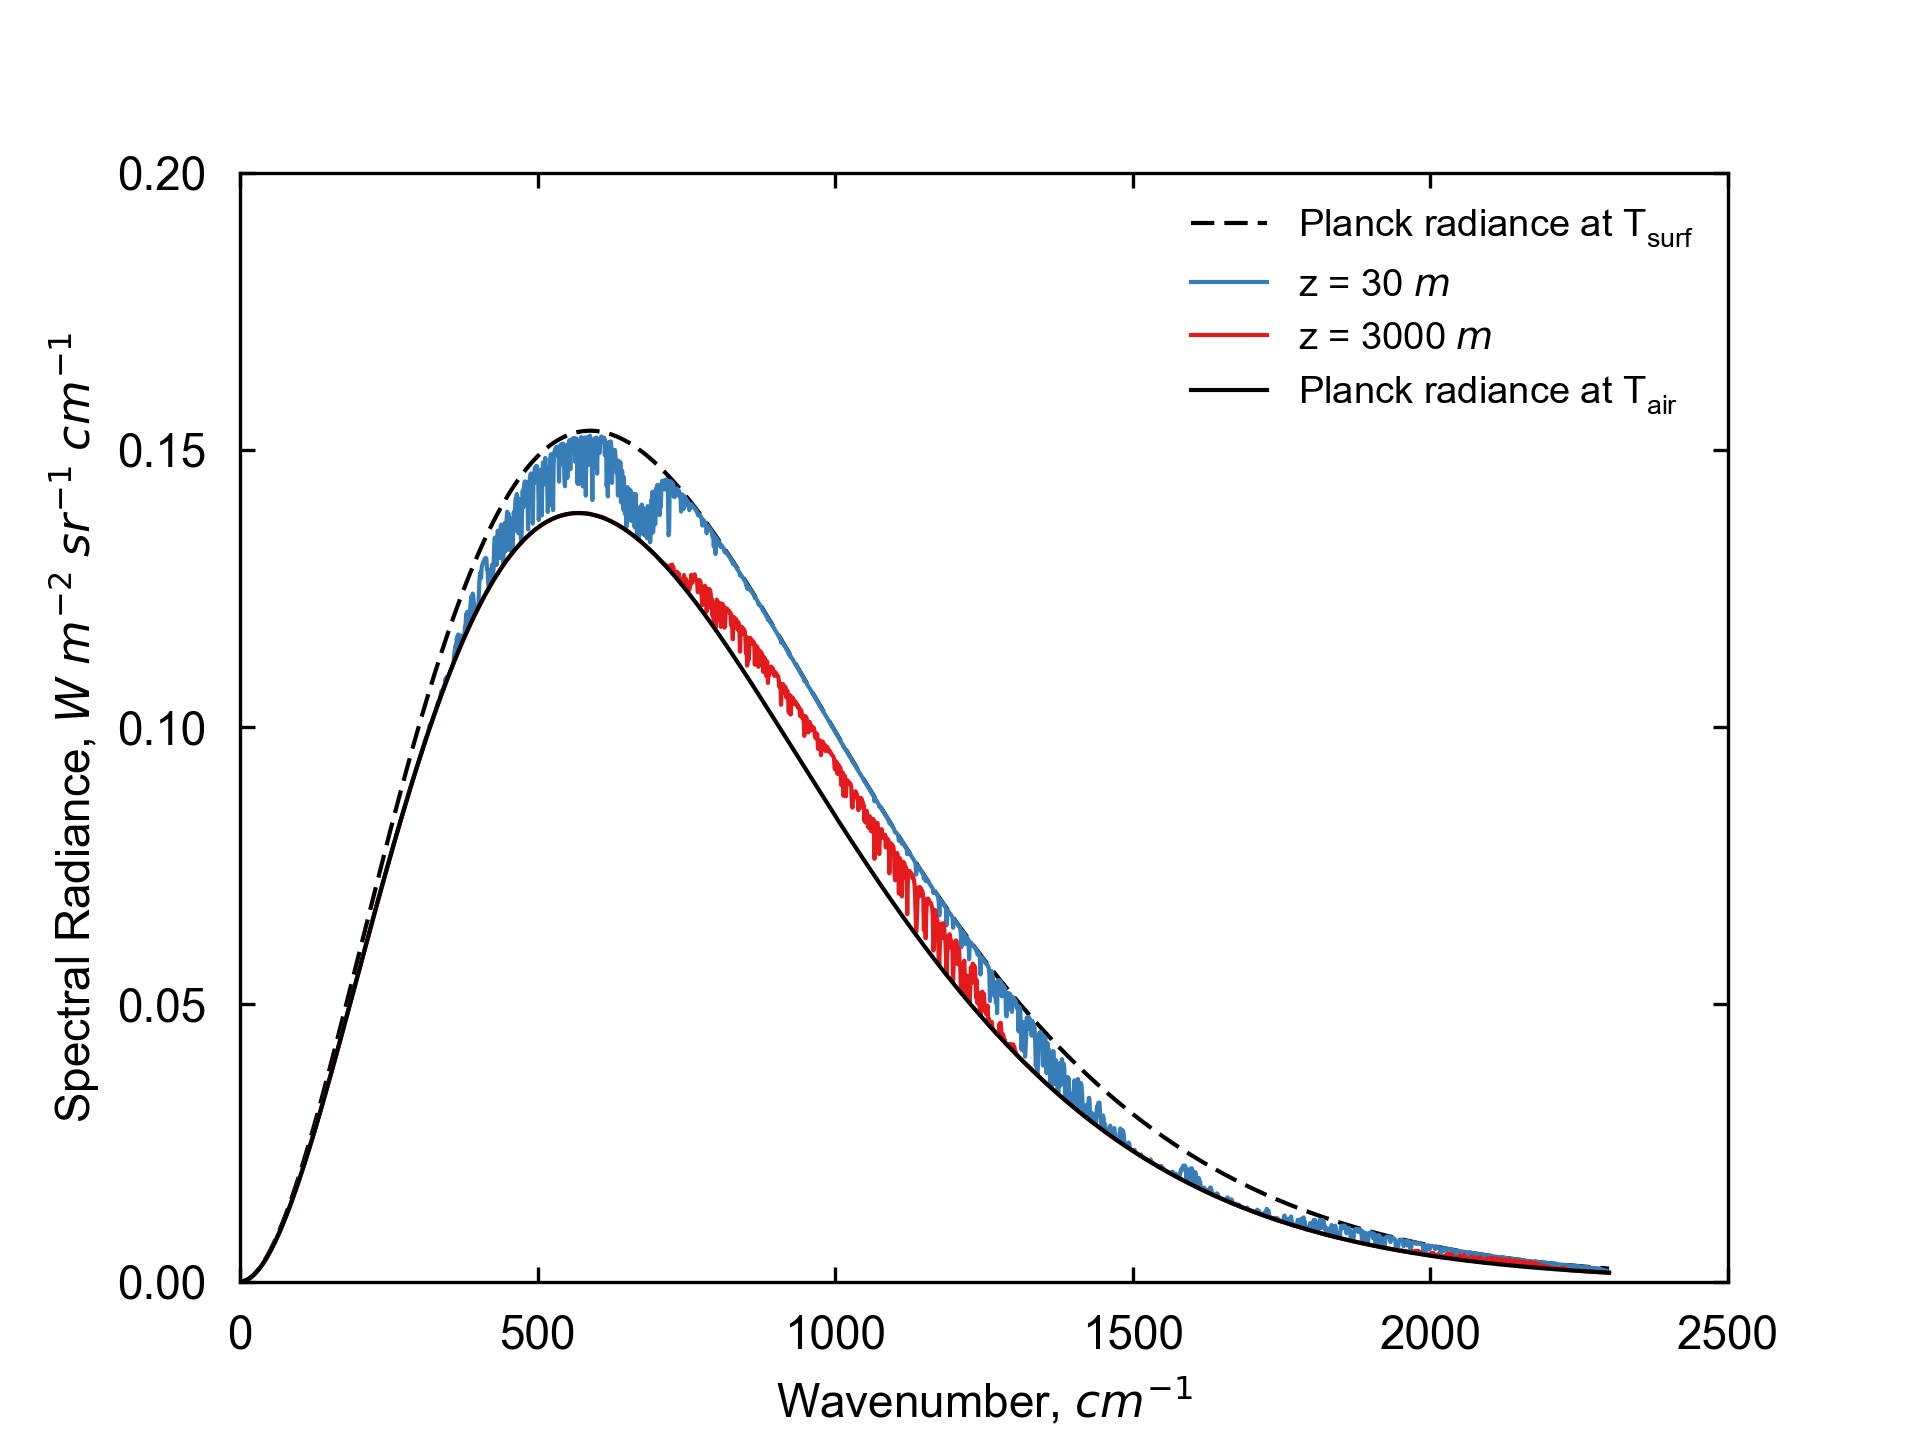
\includegraphics[width=\textwidth]{spectairtsurf}
	\caption{At-sensor spectral directional radiances computed in MODTRAN 4.1 (Berk et al., 1987) for short (30 \si{m}) and long (3000 \si{m}) path lengths ($z$) with Planck curves indicating spectral radiances at T\textsubscript{surf} = 300 \si{K} and T\textsubscript{air} = 290 \si{K}.}
	\label{spectairtsurf}
\end{figure}

Atmospheric effects can lead to differences between the 'true' radiometric T\textsubscript{surf} and the remote sensed T\textsubscript{surf} of over 10 \si{K} for satellite platforms \citep{Cooper1989} and over 6 \si{K} for near-ground sensors \citep{Meier2011}. Moreover, because atmospheric effects are a function of non-uniform and spatiotemporally variant surface and atmospheric properties, their associated errors change depending on instrument type, surface-sensor geometry, study location, and ambient conditions. As intersite and time-continuous analysis is a significant goal of most thermal remote sensed studies (urban or otherwise) these effects cannot be ignored.

Spectral transmission of longwave radiation through a given layer of atmosphere is dependent on total column absorber content (the principal broadband TIR absorbers are H\textsubscript{2}O, CO\textsubscript{2}, and to a lesser extent O\textsubscript{3}, N\textsubscript{2}O, CO, CH\textsubscript{4}, and O\textsubscript{2} \citep{Miskolczi1993}). Holding vertical absorber content constant through a layer of atmosphere, variation in band-by-band TIR transmittance with path length is greatest at the scale of an urban canyon (approximately 1 to 50 \si{\meter}), where transparent spectral bands can quickly become opaque with small changes in path length or absorber content - illustrated in Figure \ref{spectransheight}. Thus, transmittance of TIR near the surface is highly dependent on surface-sensor geometry, instrument spectral response, and atmospheric absorber content. Indeed, accurate assessment of atmospheric influence on TIR may be most complex when measured near the surface. 

\begin{figure}[H]
	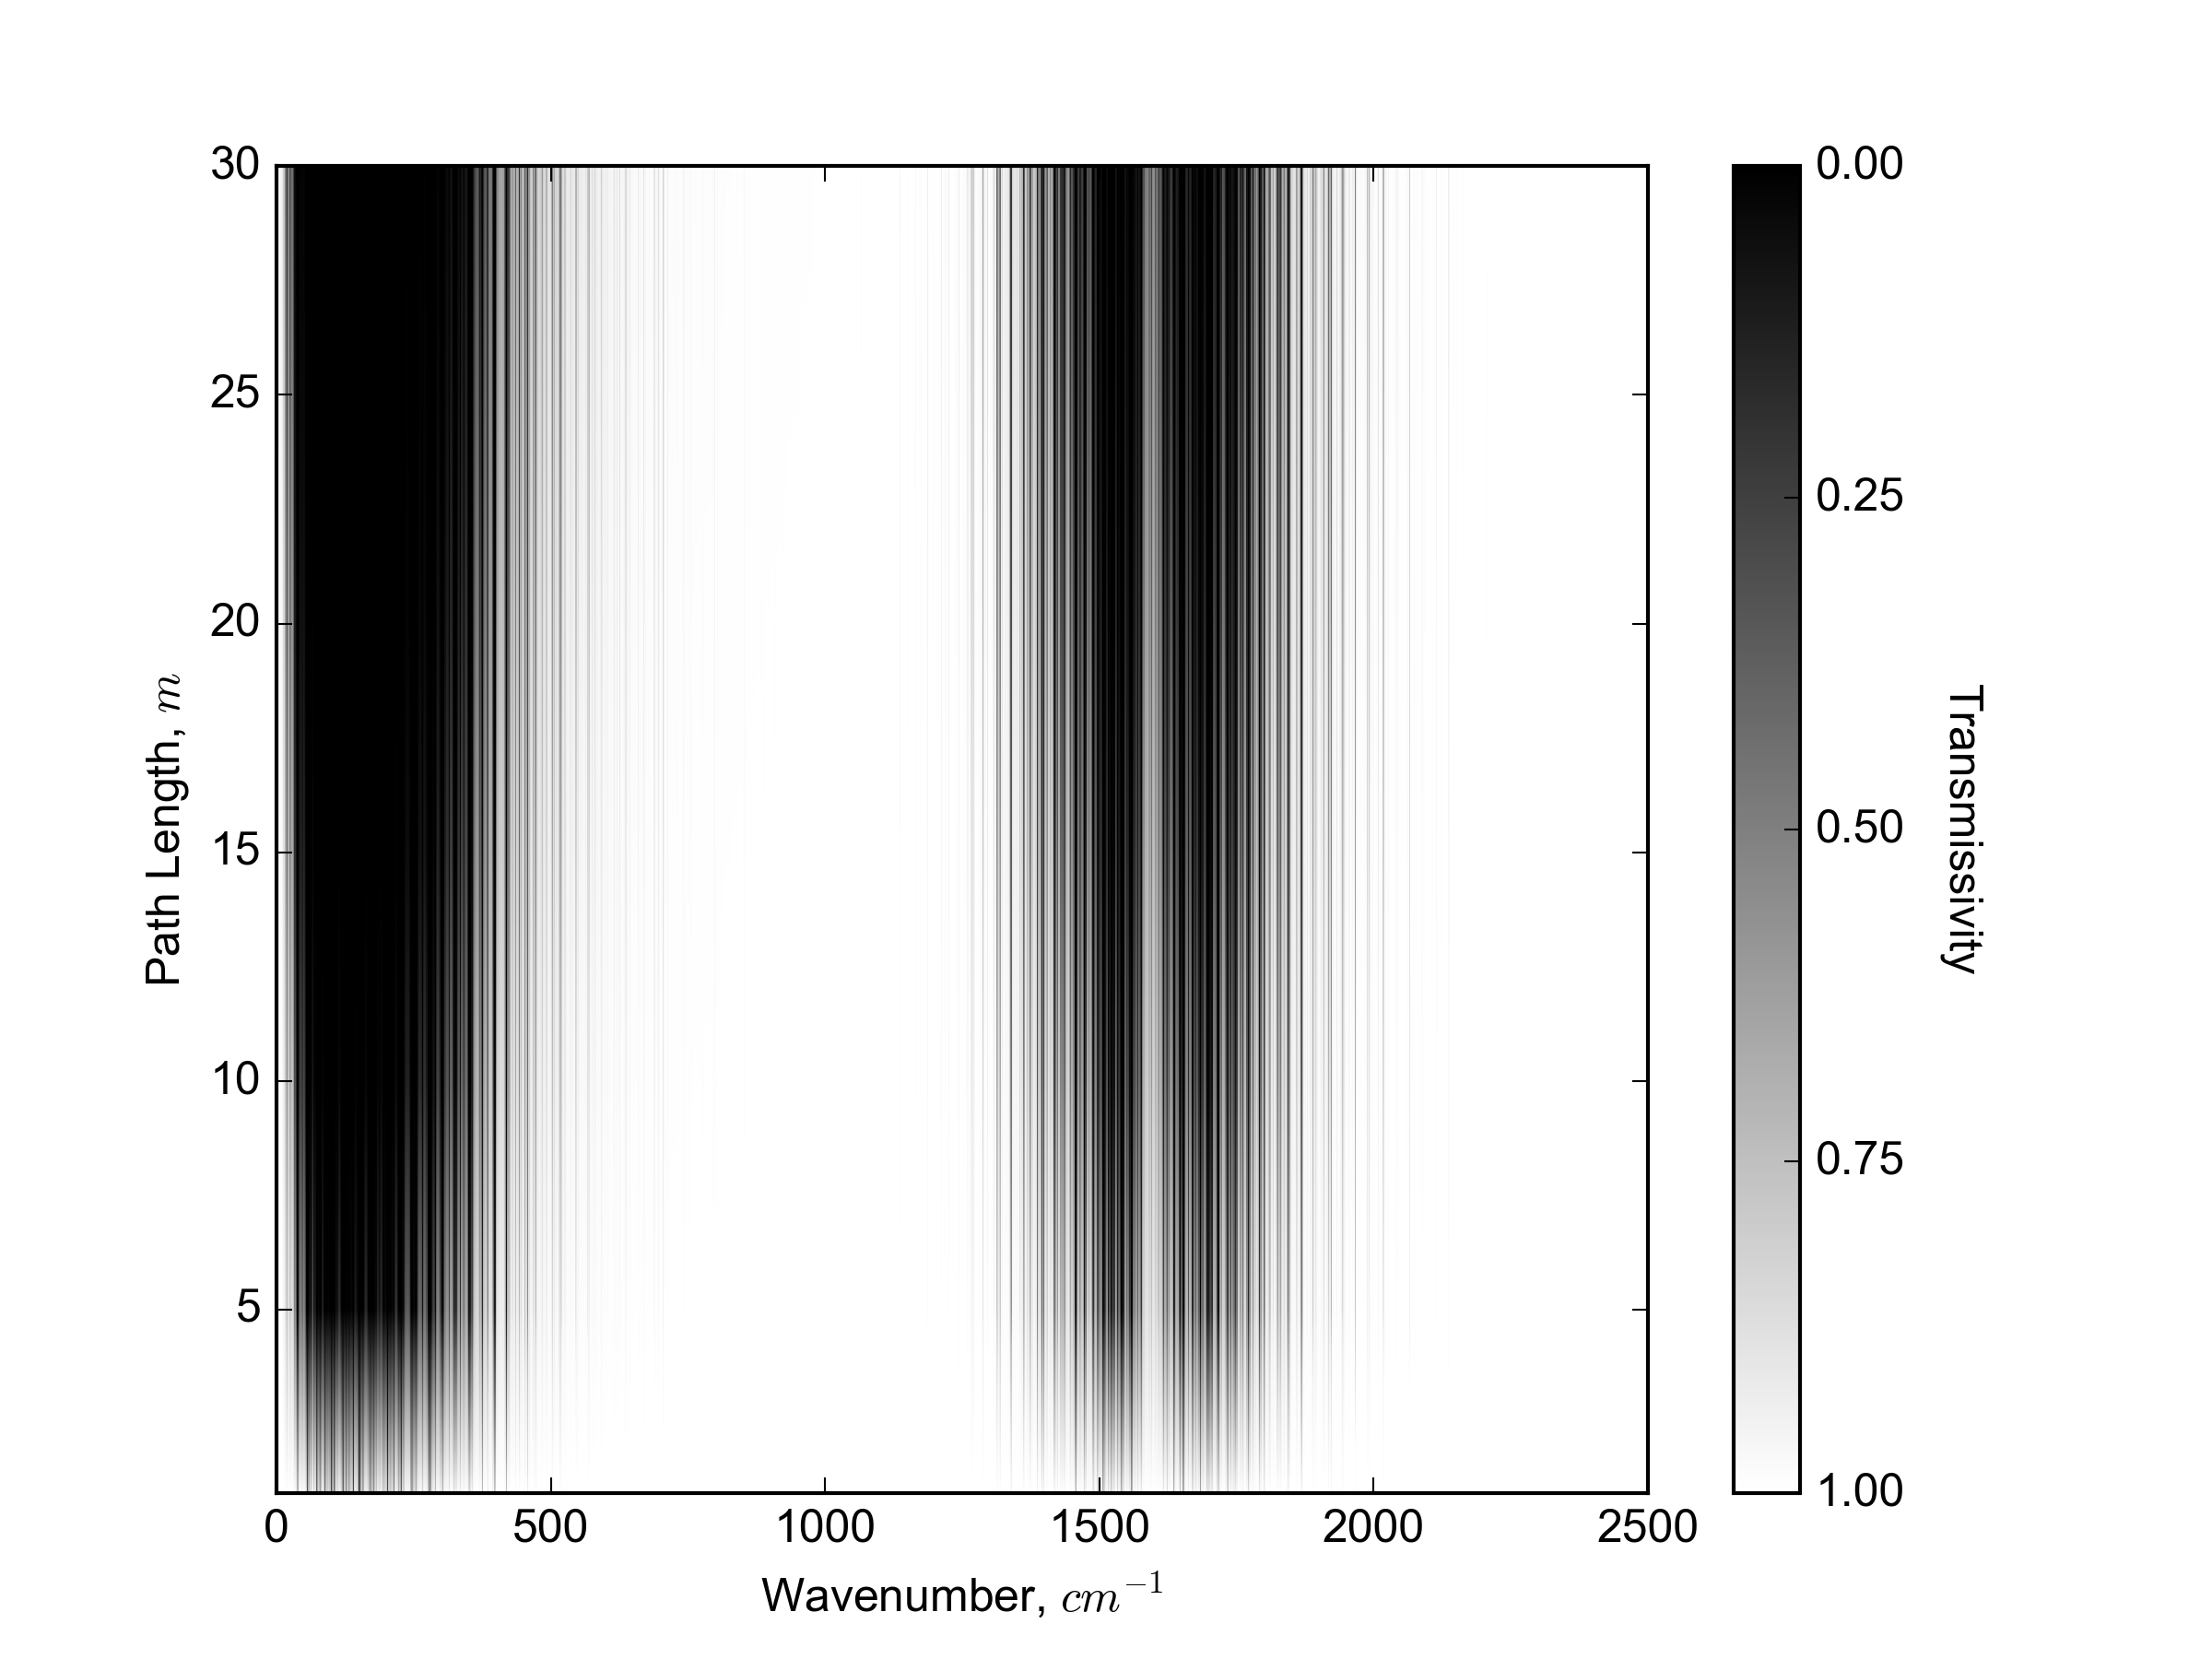
\includegraphics[width=\textwidth]{spectransheight}
	\caption{Spectral transmission of water vapor as a function of height. Model results from MODTRAN 4.1 for radiance emitted from a planar surface at 300 \si{\kelvin} through an atmosphere with water vapor content of 8 \si{\gram\per\meter\cubed}. Sampled at heights of 1, 5, 10, 15, 20, 25, and 30 \si{\meter}.}
	\label{spectransheight}
\end{figure}

\subsection{Describing radiation as received by a remote sensor}

Radiation passing through a layer of atmosphere from an emitting surface towards a sensor can be described in a number of ways: \textit{Spectral directional radiance} $R^\uparrow_z (\lambda, \theta, \phi)$, at height $ z $, wavelength $\lambda$ and from a direction defined by viewing zenith angle \(\theta\), and azimuth angle \(\phi\) is commonly written as

\begin{equation}
R^\uparrow_z (\lambda, \theta, \phi) = \tau_\lambda \epsilon_\lambda R^\uparrow_0(\lambda) + (1-\epsilon_\lambda) R^\downarrow_{sky} (\lambda) + (1-\tau_\lambda) R^\uparrow_{atm}(\lambda)
\end{equation}

\noindent where \(\epsilon\)\textsubscript{\( \lambda \)} is spectral surface emissivity, \(\tau\)\textsubscript{\( \lambda \)} is spectral "slab" transmittance through the layer between the emitting surface $( z  = 0) $ and $ z $. Directional radiances upwelling from the atmosphere $R^\uparrow_{atm}$, and the surface $R^\uparrow_0$, and downwelling from the sky $R^\downarrow_{sky}$, can be described spectrally or integrated over a waveband bounded by \(\lambda_1\) and \(\lambda_2\) as Planck's law

\begin{equation}
R(\theta, \phi) = \bigints_{\lambda_1}^{\lambda_2} R(\lambda,\theta, \phi) ~ d\lambda =\displaystyle\frac{\epsilon_\lambda C_1}{\pi \lambda^5 \left( \exp\left(\cfrac{C_2}{\lambda T}\right)\right)}
\end{equation}

\noindent where C\textsubscript{1} = $ 3.7404 \cdot 10^8 $ $ W\mu^4 m^{-2} $, C\textsubscript{2} = $ 14387 \mu K $, and $T$ is emitter temperature.

Measured by a narrow-FOV sensor mounted at height $ z $, $R^\uparrow_z (\lambda, \theta, \phi)$ passes through an instrument filter (or dome) with spectral transmittance \(\tau_d\), and is integrated over the sensor waveband to yield a \textit{directional radiance} $L_z'$ as 'seen' by the sensor

\begin{equation}
L_z' (\theta, \phi) = \int_{\lambda_1}^{\lambda_2} \tau_d(\lambda) R^\uparrow_z(\lambda) ~ d\lambda
\end{equation}

\noindent which, integrated over the hemisphere with respect to zenith \(\theta\) angle and azimuth \(\phi\) angle, yields an \textit{irradiance} $ L $ at height $ z $,

\begin{equation}
L_z = \int_{0}^{2\pi} \int_{0}^{\pi/2} L_z'(\theta, \phi) ~ \cos\theta \sin\theta ~ d\theta d\phi
\end{equation}

\subsection{Relating TIR and surface temperature}

TIR received by a remote sensor can be related to a surface temperature in a number of ways --- each producing different conceptions of T\textsubscript{surf} from different instrument and sensor types. As such, the term "surface temperature" with respect to a remote sensed TIR is vague and can refer to several definitions of "surface" and "temperature". Thus, proper terminology must be attached to land T\textsubscript{surf} inferred from TIR. Definitions and nomenclature conventions for multiple methods for T\textsubscript{surf} retrieval are discussed at length in \citet{Norman1995}.

 Irradiance $L_z$ received by a broadband hemispherical sensor (such as a pyrgeometer), can be used to infer a \textit{hemispherical brightness temperature} T\textsubscript{hem, b} through an inversion of the Stefan-Boltzmann law,

\begin{equation}
\label{stefb1}
T_{hem,~ b} = \sqrt[4]{\frac{L_z}{\sigma}}
\end{equation}

\noindent where $ \sigma $ is the Stefan-Boltzmann constant.

A \textit{directional brightness temperature} T\textsubscript{bright} $(\theta, \phi)$ from some viewing angle described by $\theta$ and $\phi$ can be inferred from directional radiance via equation \ref{stefb1} by replacing $ L_z $ with $L_z'$ multiplied by a constant. This method is commonly used to infer T\textsubscript{bright} $(\theta, \phi)$ from infrared thermometers (IRT) operating over the atmospheric window - where atmospheric effects are minimal and T\textsubscript{bright} is a reasonably accurate approximation of T\textsubscript{surf}. However, constants must be calibrated for the range of expected T\textsubscript{surf} as the relationship between $ L_z $ and $L_z'$  is not perfectly linear with respect to emitter temperature.

Inversions of uncorrected $ L_z $ or \textbf{$L_z'$} yield a temperature equal to that of a blackbody emitting the same amount of radiation as detected by the sensor. Since $ L_z $ is unlikely to be equal to $ L_0 $ and, by extension,  $L_z'$ is unlikely to be equal to $L_0'$, T\textsubscript{hem, b} at $ z = 0 $ and T\textsubscript{hem, b} at $ z $ often show significant deviation. Hence, T\textsubscript{bright} and T\textsubscript{hem, b} are generally considered only a rough approximation representation of radiometric T\textsubscript{surf}.

To retrieve a more accurate estimation of the 'true' T\textsubscript{surf}, the same inversions can be applied to TIR measurements after correction for atmospheric effects (e.g. modification of the remote sensed TIR signal to represent the same signal at $ z = 0 $ emitted from a homogeneous, isothermal, blackbody emitter) to yield a \textit{directional radiometric surface temperature} T\textsubscript{rad} from atmospheric corrected directional radiances and a \textit{hemispherical radiometric surface temperature} T\textsubscript{hem, r} from atmospherically corrected irradiances. T\textsubscript{rad} and T\textsubscript{hem, r} provide a better approximation of the ‘true’ T\textsubscript{surf} by representing the temperature at which emitting surfaces are radiating, integrated over the sensor FOV.


\subsection{Atmospheric correction of near-ground TIR} \label{Atmospheric correction of near-ground TIR}

A large number of correction routines have been developed to remove atmospheric and emissivity effects from aerial and satellite TIR signals and derive accurate T\textsubscript{rad}. Methods range from simple mono-window \citep{Qin2001} and split-window \citep{Wan1996} routines for single-channel and multi-channel remote sensors, to schemes that integrate a radiative transfer code to isolate the surface emitted signal from interfering signals. Boundary conditions are standard across most correction methods: generally requiring vertical profiles of T\textsubscript{air}, humidity, pressure, and aerosol content to remove atmospheric effects, and surface radiative properties to correct for emissivity effects. However, correction methods are often instrument (or, at the very least, platform) specific and difficult to generalize across sensor and platform types. Few methods exist for correction of ground based remote sensed TIR --- none of which are robust enough to correct irradiances measured from a near-ground wide-field-of-view (FOV) radiometer mounted to view rough terrain. 

%In part, this is due to the fact that until recently, errors inherent in radiometer measurements were large relative to atmospheric effects. However, a new breed of more accurate radiometers and thermal imagers should prompt a critical reevaluation of this assumption.

Atmospheric correction of near-ground remote sensed TIR is subject to a unique set of challenges compared to traditional satellite and aerial platforms. Wide-FOV remote sensors have complex, multiple line-of-sight (LOS) path length geometries - illustrated in Figure \ref{lineofsight} for a downward facing pyrgeometer. Surface-sensor geometry varies significantly over the sensor FOV as some path lengths intersect with raised vertical, sloped, and horizontal features. This creates the potential for non-uniform atmospheric effects over the sensor FOV and necessitates a multi-LOS correction to retrieve accurate T\textsubscript{hem, r}. In effect, with near-ground wide-FOV sensors, surface geometry is non-trivial and must be represented in atmospheric correction routines. In contrast, over a scene retrieved via satellite, spatial viability in surface geometry and LOS angle have a negligible effect on path length. Atmospheric correction routines for satellite retrieved TIR, therefore, assume uniform or single-LOS geometry because the TIR signal passes through a relatively constant volume of atmosphere over the projected sensor FOV, regardless of surface geometry.

\begin{figure}[H]
	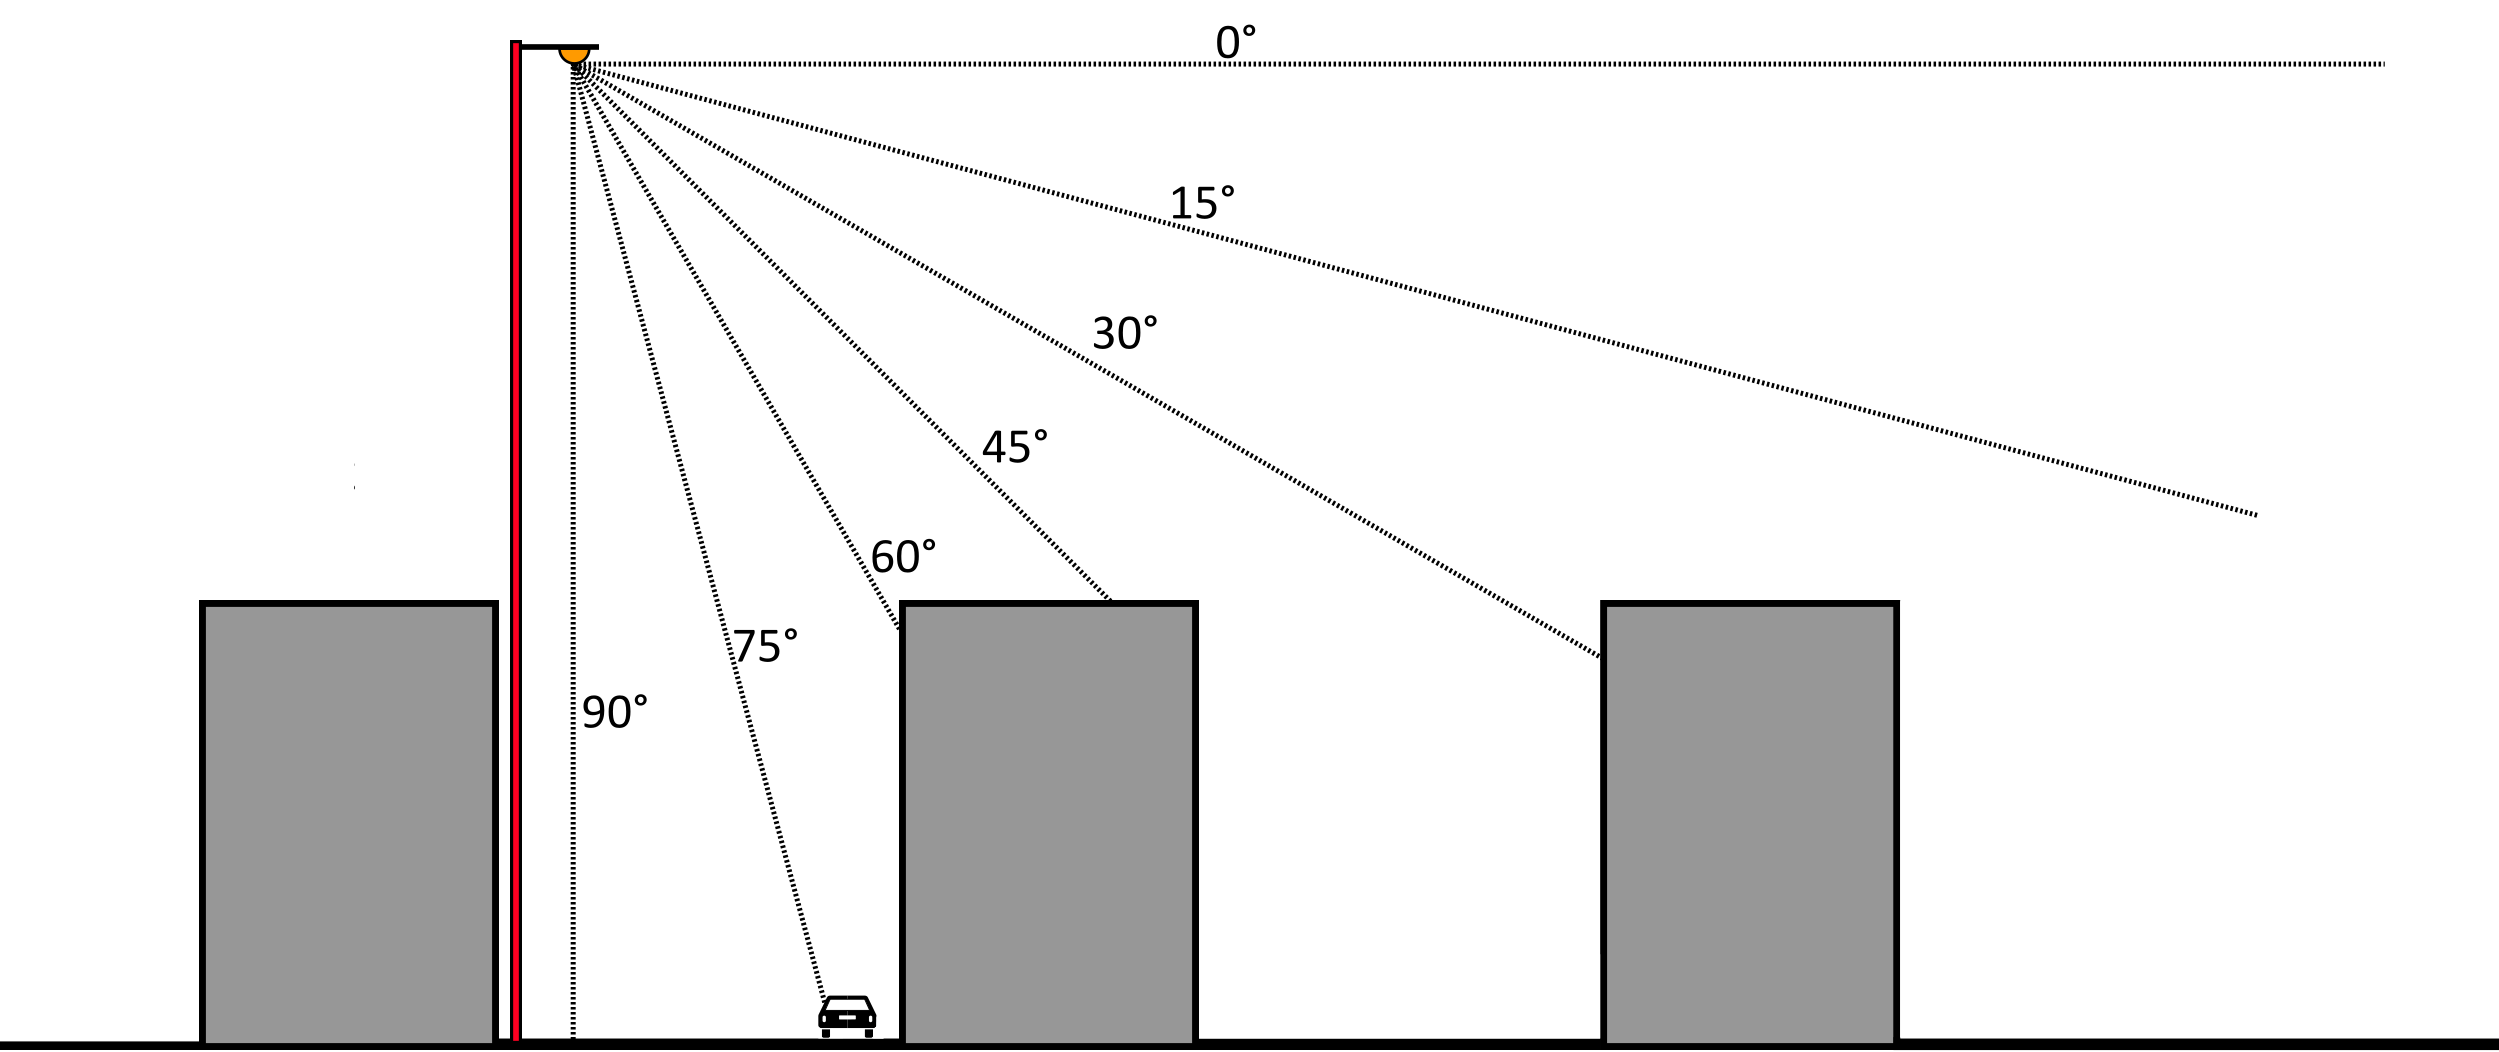
\includegraphics[width=\textwidth]{lineofsight}
	\caption{Variable path geometry inherent with wide-FOV near-ground sensor visualized over an idealized 2-dimensional urban area.}
	\label{lineofsight}
\end{figure}

Several multi-LOS correction routines have been developed to remove atmospheric effects on near-ground remote sensed TIR: \citet{Meier2011} describes a correction method for oblique angled thermal imagery of urban terrain. In the method, spatially distributed LOS geometries were calculated by linking each image pixel to the corresponding 3-d coordinates of its viewpoint on a digital building model (DBM). Path lengths were then calculated as the distance between each pixel's corresponding location on the DBM and the sensor represented as the vanishing point of a 3-dimensional pyramidic projection from the sensor's location in the DBM. A pixel-by-pixel correction was then applied to remove atmospheric effects and retrieve T\textsubscript{rad} for each pixel at 30 minute intervals, resulting in a brief, time-continuous climatology of urban T\textsubscript{rad}. However, the method uses thermal images in conjunction with a DBM to calculate path length geometries for each pixel's LOS - a technique not possible with a pyrgeometer, which returns a single integrated value over the sensor FOV. Moreover, the target instrument operates over a narrow waveband with relatively uniform spectral sensor response, reducing the magnitude and variance in atmospheric transmission over the sensor response curve. Thus, the method is not directly generalizable to correct TIR measured via pyrgeometer.

\citet{Kotani2009a} describes a method for correction of wide-FOV (pyrgeometer) TIR irradiances over a homogeneous planar surface. In this method, path lengths were calculated for six sensor heights. Radiances were then modeled using the LOWTRAN \citep{Kneizys1988} radiative transfer code initialized at $5^{\circ}$ intervals and integrated over the hemisphere to retrieve irradiances for a suite of T\textsubscript{surf}, and ambient T\textsubscript{air} and humidities. The resulting lookup table (LUT) of values is then used to correct $L_z$ and quantify atmospheric effects on remote sensed $L_z$ measured from several sensor heights. 

The two existing methods are limited to narrow-FOV thermal imagers and planar terrain respectively. Thus, for atmospheric correction of TIR upwelling from urban terrain measured via downward facing pyrgeometer a method which combines \citet{Meier2011}'s representation of complex surface geometry and \citet{Kotani2009a}'s broadband hemispherical integration is needed.

\section{A "rolling lookup table" method for hemispherical atmospheric correction}

%alt title:method to retrieve atmospherically corrected hemispherical surface temperatures from near ground TIR

The "rolling lookup-table" method described in this study uses a sensor view model in conjunction with a radiative transfer code to model hemispherical irradiances upwelling from a simplified isothermal 3-dimensional representation of the urban surface. In summary, the method (depicted in Figure \ref{flow}) uses vertical profiles of measured T\textsubscript{air} and humidity to model at-sensor spectral radiances at 5$^{\circ}$ increments over the sensor FOV for a predetermined range of possible T\textsubscript{hem, r} at each time-step. Spectral directional radiances are convolved by a dome transmittance curve, integrated over the sensor waveband, and weighted for their respective angular view factor. Weighted directional radiances are then integrated over the hemisphere and aggregated into a LUT of modeled irradiance - T\textsubscript{hem, r} pairings for each time step, unique to the vertical profile of measured T\textsubscript{air} and humidity. Finally, for each time step, measured irradiances are matched with the closest modeled irradiances in the LUT to return an atmospherically corrected radiometric hemispherical surface temperature. This process is repeated at 30 minute intervals to yield a continuous climatology of urban T\textsubscript{hem, r}. The following sections introduce the study area for which the method was developed and describe the sensor view model, radiative transfer, and post-processing steps of the correction method.

\begin{figure}[!ht]
	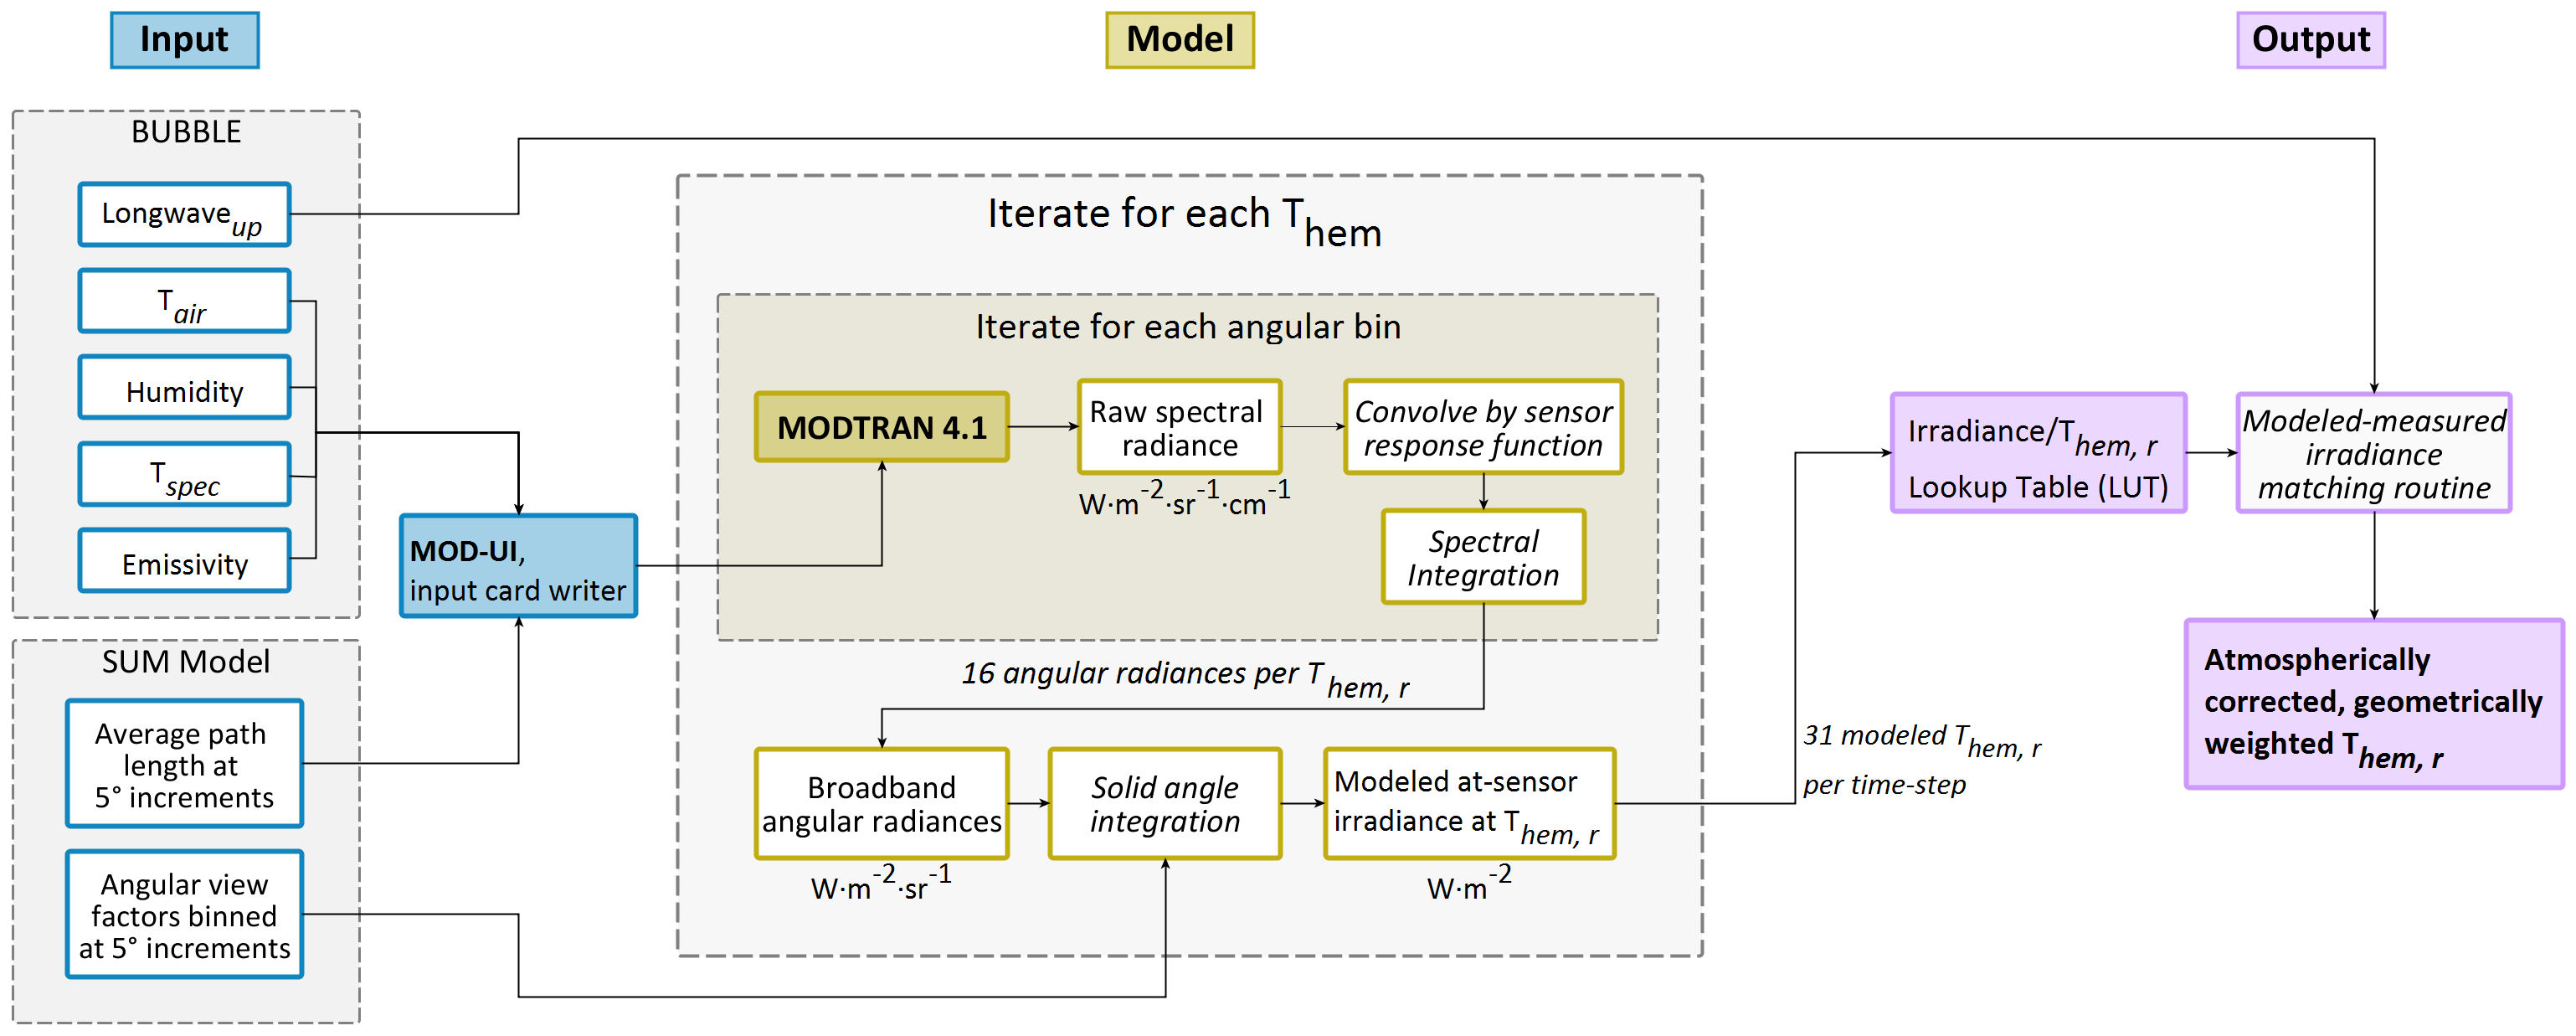
\includegraphics[width=\textwidth]{flow}
	\caption{A workflow schematic depicting the input, model, and output-processing steps of a "rolling lookup table method" for hemispherical radiometric surface temperature retrial.}
	\label{flow}
\end{figure}

\subsection{Study area}

As discussed in section \ref{Atmospheric correction of near-ground TIR}, atmospheric correction of longwave irradiances measured from downward-facing, near-ground, wide-FOV sensors must account for complex surface geometry. Thus, routines to retrieve atmospherically corrected urban T\textsubscript{hem, r} from upwelling longwave irradiances are inherently site specific. However, it is important to note that although correction \textit{magnitudes} described in this paper are not necessarily generalizable, the correction \textit{method} described in this paper can readily be adapted to different study sites, sensor types, and unique surface geometries.

With methodological generalizability in mind, a "rolling lookup table" atmospheric correction method was developed to retrieve radiometric T\textsubscript{hem, r} for a climatology of upwelling longwave irradiances measured from above the Sperrstrasse street canyon in Basel, Switzerland. The site, instrumented as a part of the Basel Urban Boundary Layer Experiment (BUBBLE) \cite{Rotach2005}, has an approximately northeast-southwest orientation and site morphology representative of local climate zone (LCZ) 2\footnote{Site surroundings can be described by the following morphological parameters: mean building height: 14.6m, plan aspect ratio: 0.54, complete aspect ratio: 1.92, local canyon aspect ratio: 1.0, and average shortwave albedo: 0.11 \cite{Rotach2005}.} \cite{Stewart2012}. LCZ classification was based on an assessment of surface characteristics in a 250 \si{\meter} circular area extending from the Sperrstrasse tower using a 1 \si{m} raster digital building model (DBM). Thus, the morphological parameters identified in \cite{Rotach2005} are representative of a majority of the pyrgeometer footprint. Vegetation was not included in the DBM, and is not represented in morphological assessment or the sensor view model, however, the street canyon and surrounding area has little vegetation.

For the eight month period between December 2001 and July 2002, a triangular lattice tower was installed within the Sperrstrasse street canyon. Its location was skewed towards the southeast facing wall near the along-canyon center of the canyon. Instruments to observe a full suite of meteorological variables and fluxes of heat, mass, and momentum are mounted at various levels on the tower. Profiles of T\textsubscript{air} and humidity were measured at seven heights extending from 2.5 \si{m} to 31.5 \si{m} above the canyon floor (with the highest observation level at approximately 2.17 times mean roof level). Upwelling and downwelling short/longwave fluxes were obtained from radiometers mounted at the lowest and highest measurement levels, with an additional downward facing pyrgeometer mounted at roof level near the center of the street canyon. In addition, during a summertime intensive observation period (IOP) an array of narrow-FOV IRTs was installed to sample representative individual facet surface temperatures (T\textsubscript{facet}).

The BUBBLE Sperrstrasse site was chosen here for two primary reasons: 1. The site provided a long-term climatology of radiation and meteorological variables for a representative mid-latitude city. This allowed for examination of urban T\textsubscript{surf}, sUHI, and atmospheric correction magnitudes over a wide range of representative mid-latitude conditions. 2.  Inclusion of T\textsubscript{facet} over the IOP allows for investigation of the effect of sensor FOV and viewing direction on remote sensed urban T\textsubscript{surf} for common methods for urban T\textsubscript{surf} retrieval. This directional dependence of urban T\textsubscript{surf} - termed "effective anisotropy" - refers to the notion that a remote sensed TIR signal can vary based on the combined effects of surface-sensor-sun geometry and the convoluted, 3-dimensional structure of the urban surface \cite{Voogt1998a}. Facet surface temperatures measured during the summertime IOP allow for direct climatological comparison of T\textsubscript{hem, r} to common remote sensed representations of the urban surface calculated from weighted averages of wall (T\textsubscript{wall}), road (T\textsubscript{road}), and roof (T\textsubscript{roof}) temperatures. Plan and complete aspect ratios are used to derive weightings for nadir remote sensed (T\textsubscript{plan}) and complete (T\textsubscript{comp}) representations of urban surface temperature - described in Table \ref{weightings}. T\textsubscript{comp} represents a complete urban T\textsubscript{surf}, where facet temperatures are averaged based on their proportion of the complete urban surface area, while T\textsubscript{plan} represents the Sperrstrasse site as viewed by a narrow-FOV remote sensor in the nadir. To facilitate comparison over the IOP, T\textsubscript{hem, r} and T\textsubscript{plan} were divided by T\textsubscript{comp} and averaged over the IOP to yield normalized mean T\textsubscript{hem, r} and T\textsubscript{plan} at 30-minute intervals. Through comparison of T\textsubscript{hem, r} to T\textsubscript{plan} and T\textsubscript{comp} we investigate the effect of sensor-surface geometry on remote sensed urban T\textsubscript{surf} and quantify directional biases in common urban T\textsubscript{surf} measurements. 

\begin{table}[H]
	\centering
	\caption{Weights applied to individual facet temperature components in to calculate complete and nadir temperatures for the Basel Sperrstrasse street canyon.}
	\label{weightings}
	\begin{tabular*}{\textwidth}{l@{\extracolsep{\fill}} p{1cm}p{1cm}p{1cm}p{1cm}p{1.6cm}}
		\toprule 
		& Road & Northwest & Southeast & Northwest & Southeast \\ 
		&  & Roof & Roof & Wall & Wall \\ 	\midrule
		Complete (T\textsubscript{comp}) & 0.33 & 0.16 & 0.16 & 0.16 & 0.16 \\ 
		Nadir (T\textsubscript{plan}) & 0.46 & 0.27 & 0.27 & 0.00 & 0.00 \\ 
		\bottomrule
	\end{tabular*} 
\end{table}

\subsection{Modeling path lengths of 3-dimensional terrain}

The sheer number of unique path length geometries inherent with wide-FOV radiometry of urban areas makes full 3-dimensional radiative transfer simulation difficult and computationally intensive - particularly when correcting a long-term climatology of irradiances or T\textsubscript{hem, r}. In this method, to improve efficiency, radiances are calculated for azimuthally averaged path lengths that represent average surface-sensor geometry for each solid angle "slice" of the sensor FOV. Thus, hemispherical radiative transfer is reduced to a 2-dimensional problem similar to that shown in Figure \ref{23radtran}. This greatly reduces the computational time required to model each irradiance - T\textsubscript{hem, r} pairing, as angular radiances can be computed as a function of zenith angle alone and subsequently weighted and integrated 3-dimensionally over the hemisphere. 

To calculate surface-sensor geometries, the Surface-Sensor-Sun Urban Model (SUM) \citep{Soux2004} is initialized with a simplified, orthogonal 3-dimensional DBM that represents surface geometry of the surrounding area. SUM uses a four-dimensional array to represent surface morphology with three spatial dimensions ($x$, $y$, and $z$), with $z$ representing height above the $x$, $y$ plane. An additional fourth dimension is used to store information describing each cell (in this case, distance from the point to the sensor). After specifying sensor position and FOV, the model determines which patches have an unobstructed line of sight to the sensor and calculates distance from "seen" patches to the sensor. Path lengths are binned at 5$^{\circ}$ increments of zenith angle and averaged to return an azimuthally-independent mean path length for each bin. In addition, while retrieving path length geometries, SUM calculates view factors for each solid angle "slice", which are later used to weight angular radiances in the hemispherical integration post-processing steps.

\begin{figure}[H]
	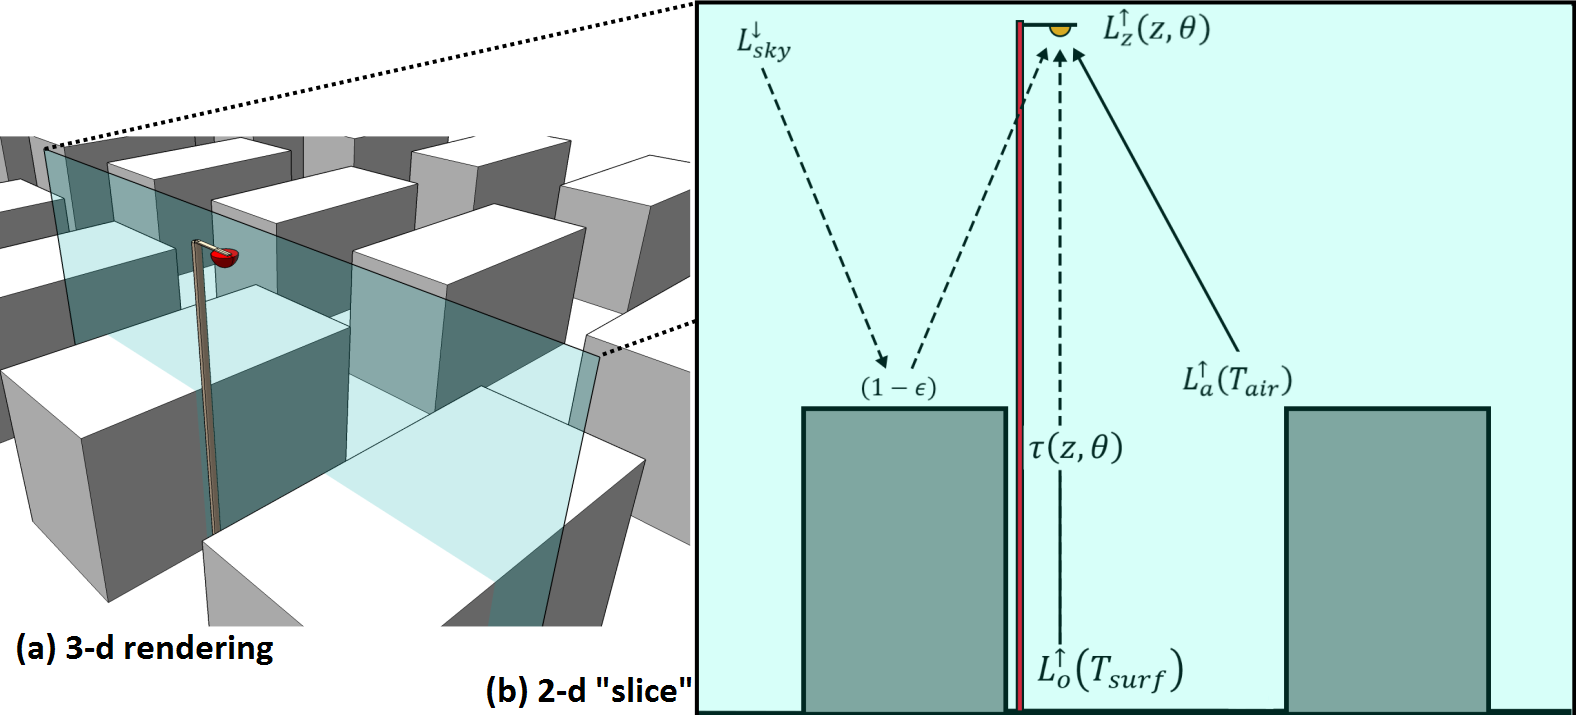
\includegraphics[width=\textwidth]{23radtran}
	\caption{Path lengths over an urban surface. Left: a downward radiometer mounted above a simplified three-dimensional urban surface (Left) and the component radiances and path lengths from a vertical slice (Right). Dotted lines indicate radiation streams subject to absorption by the intervening atmospheric layer.}
	\label{23radtran}
\end{figure}

\subsection{Modeling hemispherical irradiances}
With path length geometries calculated in SUM, irradiances are modeled for each time step using version 4.1 of the MODerate resolution atmospheric TRANsmission radiative transfer code (MODTRAN) \citep{Berk1987}. At each time-step, a range of possible temperatures is specified (T\textsubscript{spec}) based on T\textsubscript{hem, b} calculated from the measured irradiance with

\begin{equation}
	T_{spec, ~min} = T_{hem, ~b} - 6 ~K 
\end{equation}

\noindent defining a minimum T\textsubscript{spec} before iterating over

\begin{equation}
T_{spec, ~i} = T_{spec, ~min} + \displaystyle\sum_{i = 1}^{n} 0.5n, ~1 \leq n \leq 32
\end{equation}

\noindent to retrieve a LUT of T\textsubscript{spec}. 

After the LUT is defined, at-sensor spectral radiances for each path length/zenith angle are modeled at an emissivity of 0.95 over a waveband of 0 - 2300 \si{cm^{-1}} for each T\textsubscript{spec}. Profiles of T\textsubscript{air} and humidity are retrieved from 30 \si{\minute} averages of conditions observed at the Sperrstrasse site. Aerosol, trace gas absorber, and above-sensor T\textsubscript{air} and humidity conditions are defined by the mid-latitude summer standard atmosphere when daytime T\textsubscript{air, max} \textgreater 10 \si{\degreeCelsius} (the mid-latitude winter profile is substituted on days where T\textsubscript{air, max} \textless 10 \si{\degreeCelsius}) \citep{Kantor1962}. 

In this method, a "typical" longwave bandpass, approximately 250 - 2300 \si{\centi\meter^{-1}} (4 - 42 \si{\micro\meter}), was extended to include much smaller wavenumber (longer wavelengths). This was done for two reasons: 1) To accurately represent broadband spectral longwave emission curves, which show significant emittance in wavenumber smaller than 250 \si{cm^{-1}} (wavelengths longer than 42 \si{\micro\meter}). 2) To replicate the spectral signal "seen" by a silicone-domed pyrgeometer, which continues to transmit radiation at wavenumber \textless 250 \si{cm^{-1}} (wavelengths \textgreater 42 \si{\micro\meter}). A "typical" longwave bandpass underestimates a pyrgeometer signal by approximately 7 - 10 \si{\watt\per\square\meter}, depending on emitter temperature. A comparison of ‘typical’ and ‘extended’ longwave bandpasses is shown in Figure \ref{dometrans}.

\begin{figure}[H]
	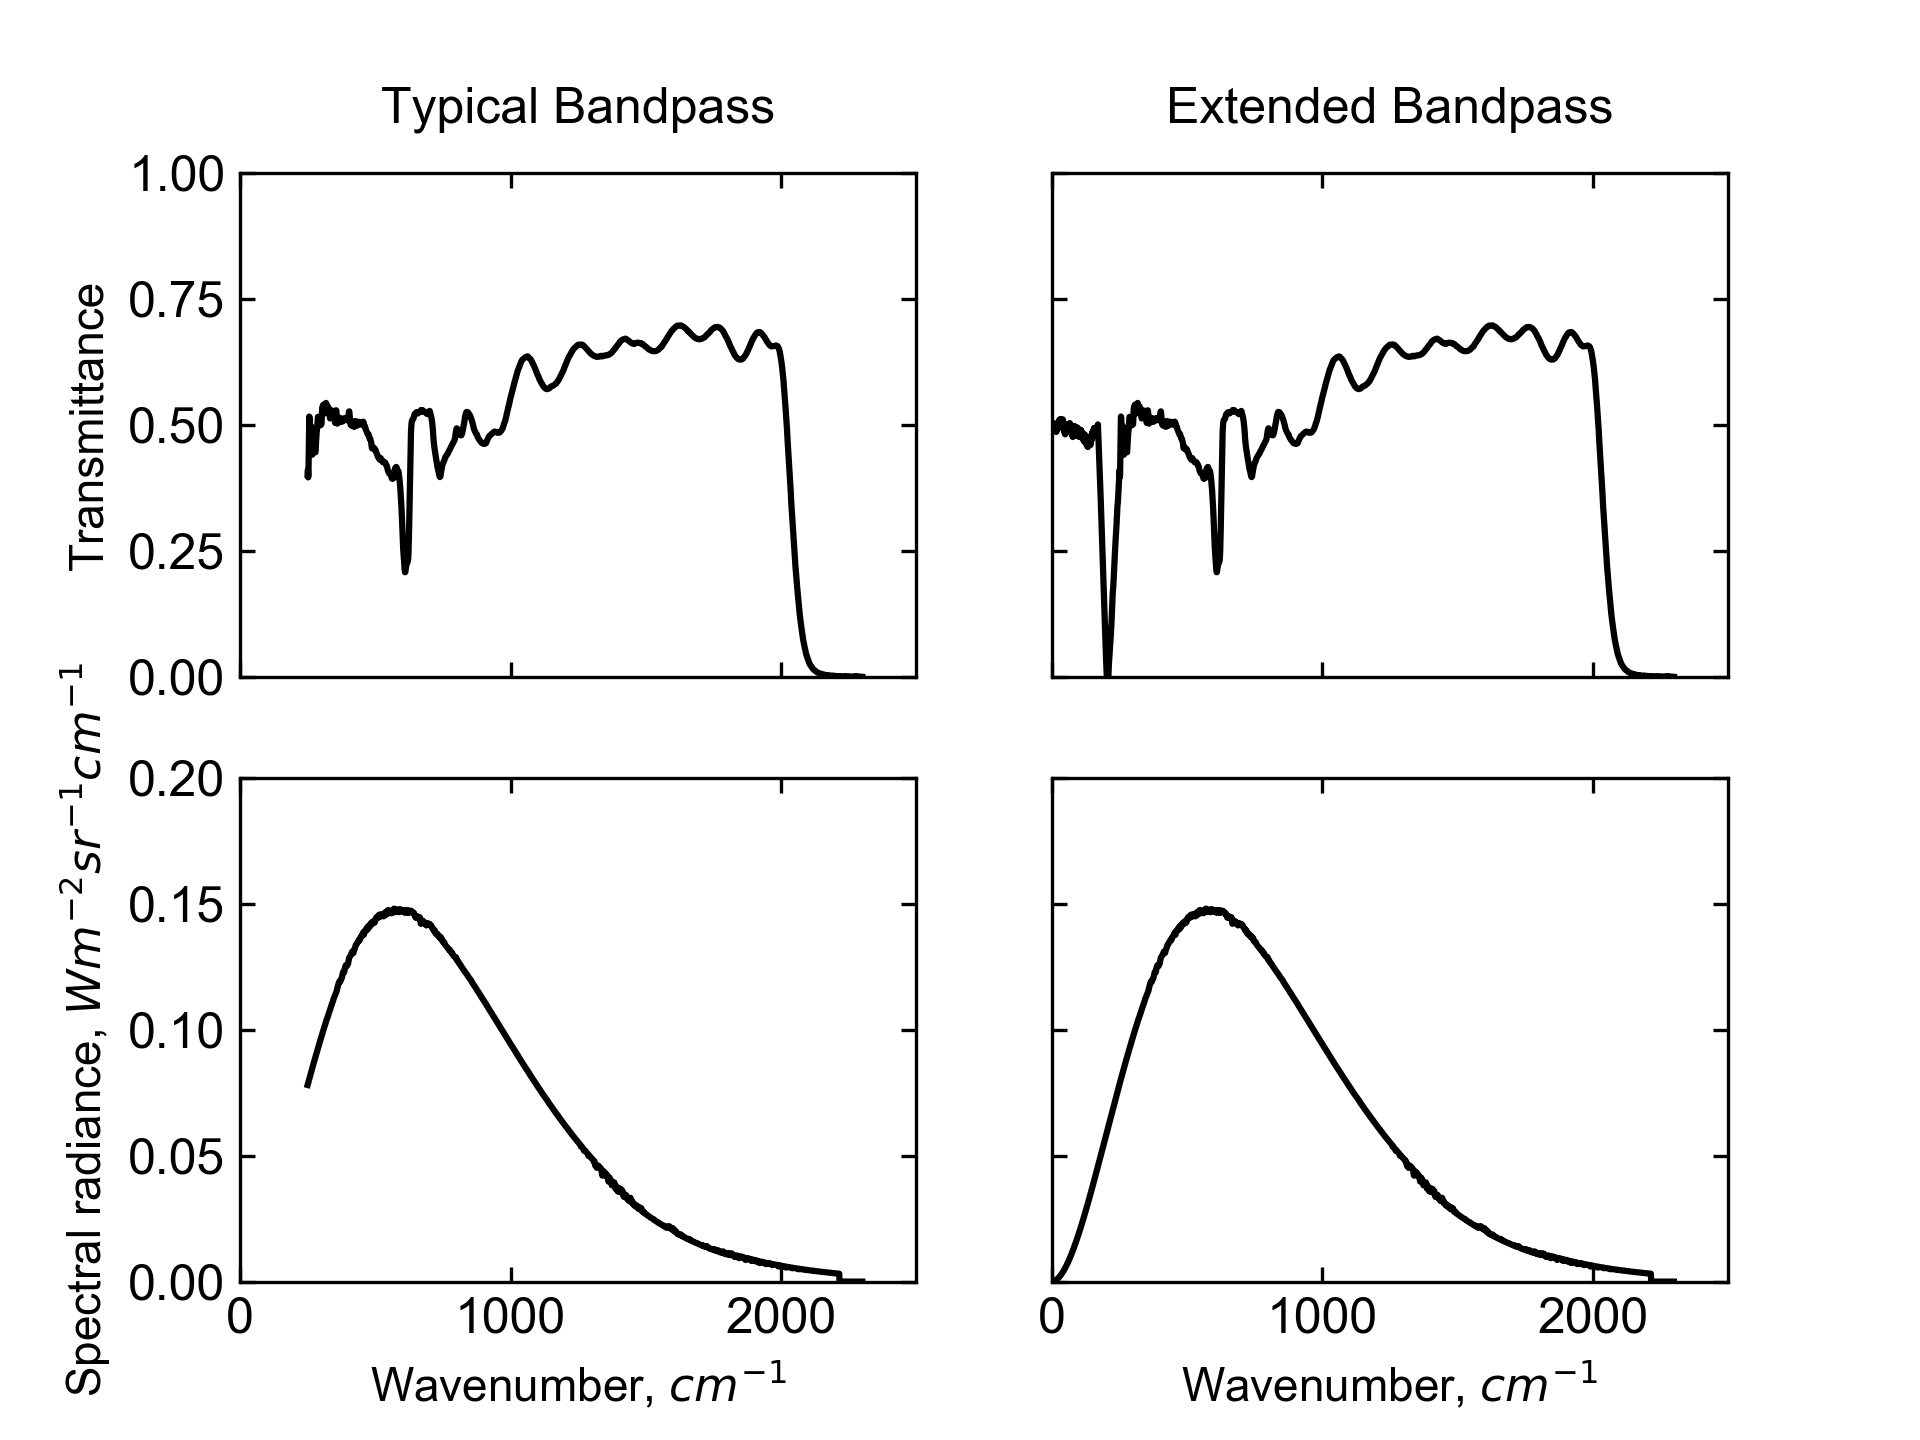
\includegraphics[width=\textwidth]{dometrans}
	\caption{A comparison of dome transmittance for a Kipp \& Zonen silicone domed pyrgeometer (data supplied by Kipp \& Zonen, \textit{pers. comm.}) and at-sensor radiance (T\textsubscript{surf} = 300 \si{K}, T\textsubscript{air} = 300 \si{K}, $z$ = 30 \si{m})  for "typical" and extended bandpasses.}
	\label{dometrans}
\end{figure}

At-sensor spectral radiances computed by MODTRAN are convolved by a dome transmittance curve and integrated over the bandpass via 

\begin{equation}
\label{work1}
	L'_z (\theta, \phi) = \frac{\bigints_{\nu_1}^{\nu_2} R(\theta, \phi, \lambda) ~ r(\lambda) ~ d\lambda}{\overline{r}}
\end{equation}

\noindent to yield a directional radiance $ L'_z $ for each $\theta$ over a waveband of $\nu_1 $= 0 \si{\per\centi\meter} to $\nu_2$ = 2300 \si{cm^{-1}}. $ \overline{r} $ is Planck weighted mean broadband sensor response computed as,

\begin{equation}
\label{meansens}
\overline{r} = \cfrac{\int R(\lambda) ~ r(\lambda)~d\lambda}{\int R(\lambda) ~ d\lambda}
\end{equation}

\noindent where $ R(\lambda) $ is spectral radiance computed from a Planck function at an approximated emitter temperature and $r (\lambda)$ is spectral sensor response. 

$ L'_z (\theta) $ are then multiplied by their associated angular view factor weighting ($\Phi$) and integrated over the hemisphere to yield an irradiance $ L_z $ for the target T\textsubscript{hem, r}

\begin{equation}
\label{work2}
	L_z (T\textsubscript{spec}) = \int_{0}^{2\pi}\int_{0}^{\pi/2} L'_z (\phi, \theta) ~ \Phi (\phi) ~ d\theta d\phi
\end{equation}

$L_z (T\textsubscript{spec}) $ is representative of at-sensor irradiance upwelling from the urban surface described in SUM at the target specified temperature T\textsubscript{hem, r} for the measured T\textsubscript{air}, humidity, aerosol, and trace gas profile. The process is repeated to retrieve $L_z$ for the range of potential T\textsubscript{hem, r} at the given time-step. Irradiance - T\textsubscript{hem, r} pairings are then aggregated into a LUT. Finally, the measured irradiance is matched with its closest modeled irradiance to yield an atmospherically corrected, radiometric hemispherical surface temperature for the given time step. The workflow is repeated at 30 \si{\minute} intervals to yield a continuous time series of T\textsubscript{hem, r}. Atmospheric correction magnitudes can then be calculated as the difference between T\textsubscript{hem, r} and T\textsubscript{hem, b}, with T\textsubscript{hem, b} calculated via equation \ref{stefb1}.

\section{Evaluation of the method using profiles of upwelling longwave radiation over a homogeneous flat surface} \label{sensitivity}

MODTRAN has been shown to effectively model near-ground radiative transfer at urban canyon scale path lengths in 2-dimensions \citep{Hoch2005, Hoch2007}. However, the method described in this paper accounts for complex 3-dimensional surface geometry, which can exert significant influence on atmospheric transmittance. In addition, the method includes significant post-processing to weight and integrate point-to-point spectral directional radiances to derive 3-dimensional, hemispherical irradiances. Thus, prior to deriving a climatology of urban T\textsubscript{hem, r}, the method was evaluated using profiles of upwelling longwave irradiances measured over a simple flat surface.

%Although downward facing pyrgeometers mounted at different heights do not have the same radiative source area. Over a simple relatively homogeneous surface, the signal measured by each sensor should be radiating from an approximately isothermal surface area. As such, differences in the upwelling longwave signal between sensor heights (a phenomenon termed longwave divergence) are solely the result of differential atmospheric effects, which should be accounted for by the model.

For a continuous 14-day period, profiles of up/downwelling short/longwave radiation, T\textsubscript{air}, and humidity measured from 2 \si{m}, 10 \si{m}, and 30 \si{m} were obtained from an instrumented tower in Payerne, Switzerland. The tower, installed over a cultivated field as a part of the Baseline Surface Radiation Network (BSRN), is located approximately 100 \si{\kilo\meter} southwest of the BUBBLE Sperrstrasse tower and is subject to similar summertime conditions as the study site. The study period was chosen to include a comprehensive range of T\textsubscript{surf}, T\textsubscript{air}, humidities, and cloud coverages to represent typical summertime conditions over which atmospheric effects on TIR can vary significantly. To evaluate the method, we used a modified version of the workflow described in Figure \ref{flow}. First, azimuthally averaged path lengths over a flat surface were calculated in SUM at 5\si{\degree} increments of zenith angle over the sensor FOV for the 10 \si{\meter} and 30 \si{\meter} sensors. For each time step, T\textsubscript{hem, b} calculated from the lowest $L_z$ measurement was used to model irradiances at 10 \si{m} and 30 \si{m} at 30 \si{\minute} intervals using concurrent profiles of T\textsubscript{air} and humidity. Daytime T\textsubscript{air} observed at the highest measurement level was anomalously high compared to typical summertime lapse rates above flat vegetated terrain \citep{Oke1987}. This warm bias in T\textsubscript{air} measured at 30 \si{\meter} is observed even under high wind velocities, where one would expect little vertical difference in temperature and certainly not a strong temperature inversion. The fact that the observed warming bias remains relatively constant over the 14-day study period prompted a slight modification to ensure the T\textsubscript{air} profile between 10 \si{\meter} and 30 \si{\meter} was representative of the neutral or weakly unstable daytime conditions. It is likely that these modifications better represent the actual T\textsubscript{air} profile in the layer between 10 \si{\meter} and 30 \si{\meter} than a simple interpolation between the 10 \si{\meter} T\textsubscript{air} measurement and the anomalously warm 30 \si{\meter} T\textsubscript{air} measurement. 

Contrary to the findings in \citet{Kotani2009a}, an isothermal atmospheric profile was not sufficient to accurately model upwelling fluxes over flat terrain. Although thermal stratification is relatively small by day in an urban canyon \citep{Nakamura1988} --- where strong microscale contrasts in T\textsubscript{surf} foster strong canyon mixing and neutral stability --- the large daytime T\textsubscript{surf} - T\textsubscript{air} differential and the path length/transmittance gradient can create large differences in upwelling longwave forced by inter-canyon thermal contrasts - a phenomenon termed radiative divergence. By underestimating near-surface T\textsubscript{air} and overestimating roughness-layer T\textsubscript{air}, daytime divergences are underestimated by an isothermal profile. As such, a full canyon T\textsubscript{air} and humidity profile is preferred to most accurately model near ground fluxes.

Modeled and measured upwelling longwave at 10 \si{m} and 30 \si{m} fluxes and divergences - calculated as the difference between 30 \si{\meter} and 10 \si{\meter} fluxes - are compared in Figure \ref{fluxes}. Both fluxes and divergences show strong correlation, thus we conclude: First, irradiances measured near screen level (approximately 2 \si{\meter} above ground level) do not include significant atmospheric influence - as T\textsubscript{hem, b} inferred from $L_{z=2~\si{\meter}}$ was sufficient for modeling irradiances at 10 \si{m} and 30 \si{m}. As such, T\textsubscript{hem, b} and T\textsubscript{hem, r} are reasonably equal when $z$ = 2 \si{m}. However, it should be noted that in urban areas a 2 \si{m} sensor is not sufficiently representative of canyon geometry and should not be used to derive urban T\textsubscript{hem, r}. Second, MODTRAN can accurately model longwave fluxes and divergences above a flat, homogeneous surface over a wide range of temperatures, humidities, and cloud coverages and large contrasts in near-ground stability. At 30 \si{\meter} under typical summertime profiles of humidity, CO\textsubscript{2}, and O\textsubscript{3}, view factor weighted hemispherical transmittance over a flat surface is approximately 55\% - meaning 45\% of a broadband hemispherical TIR signal at 30 \si{\meter} is emitted by the atmosphere, rather than the target surface. As such, it is imperative that T\textsubscript{air} profiles are well represented in MODTRAN to accurately model the atmospheric component of remote sensed TIR signal. As profiles of T\textsubscript{air} in the layer between the surface and the sensor at the Sperrstrasse site are generally subject to neutral or weakly unstable conditions, with only rare stable stratifications, urban longwave divergences are likely to be smaller than those observed in this evaluation - and well approximated by MODTRAN. Thus, provided path length geometries are accurately replicated in by the sensor view model, we can reasonably assume that the method has similar effectiveness at the urban site.

\begin{figure}[H]
	\centering
	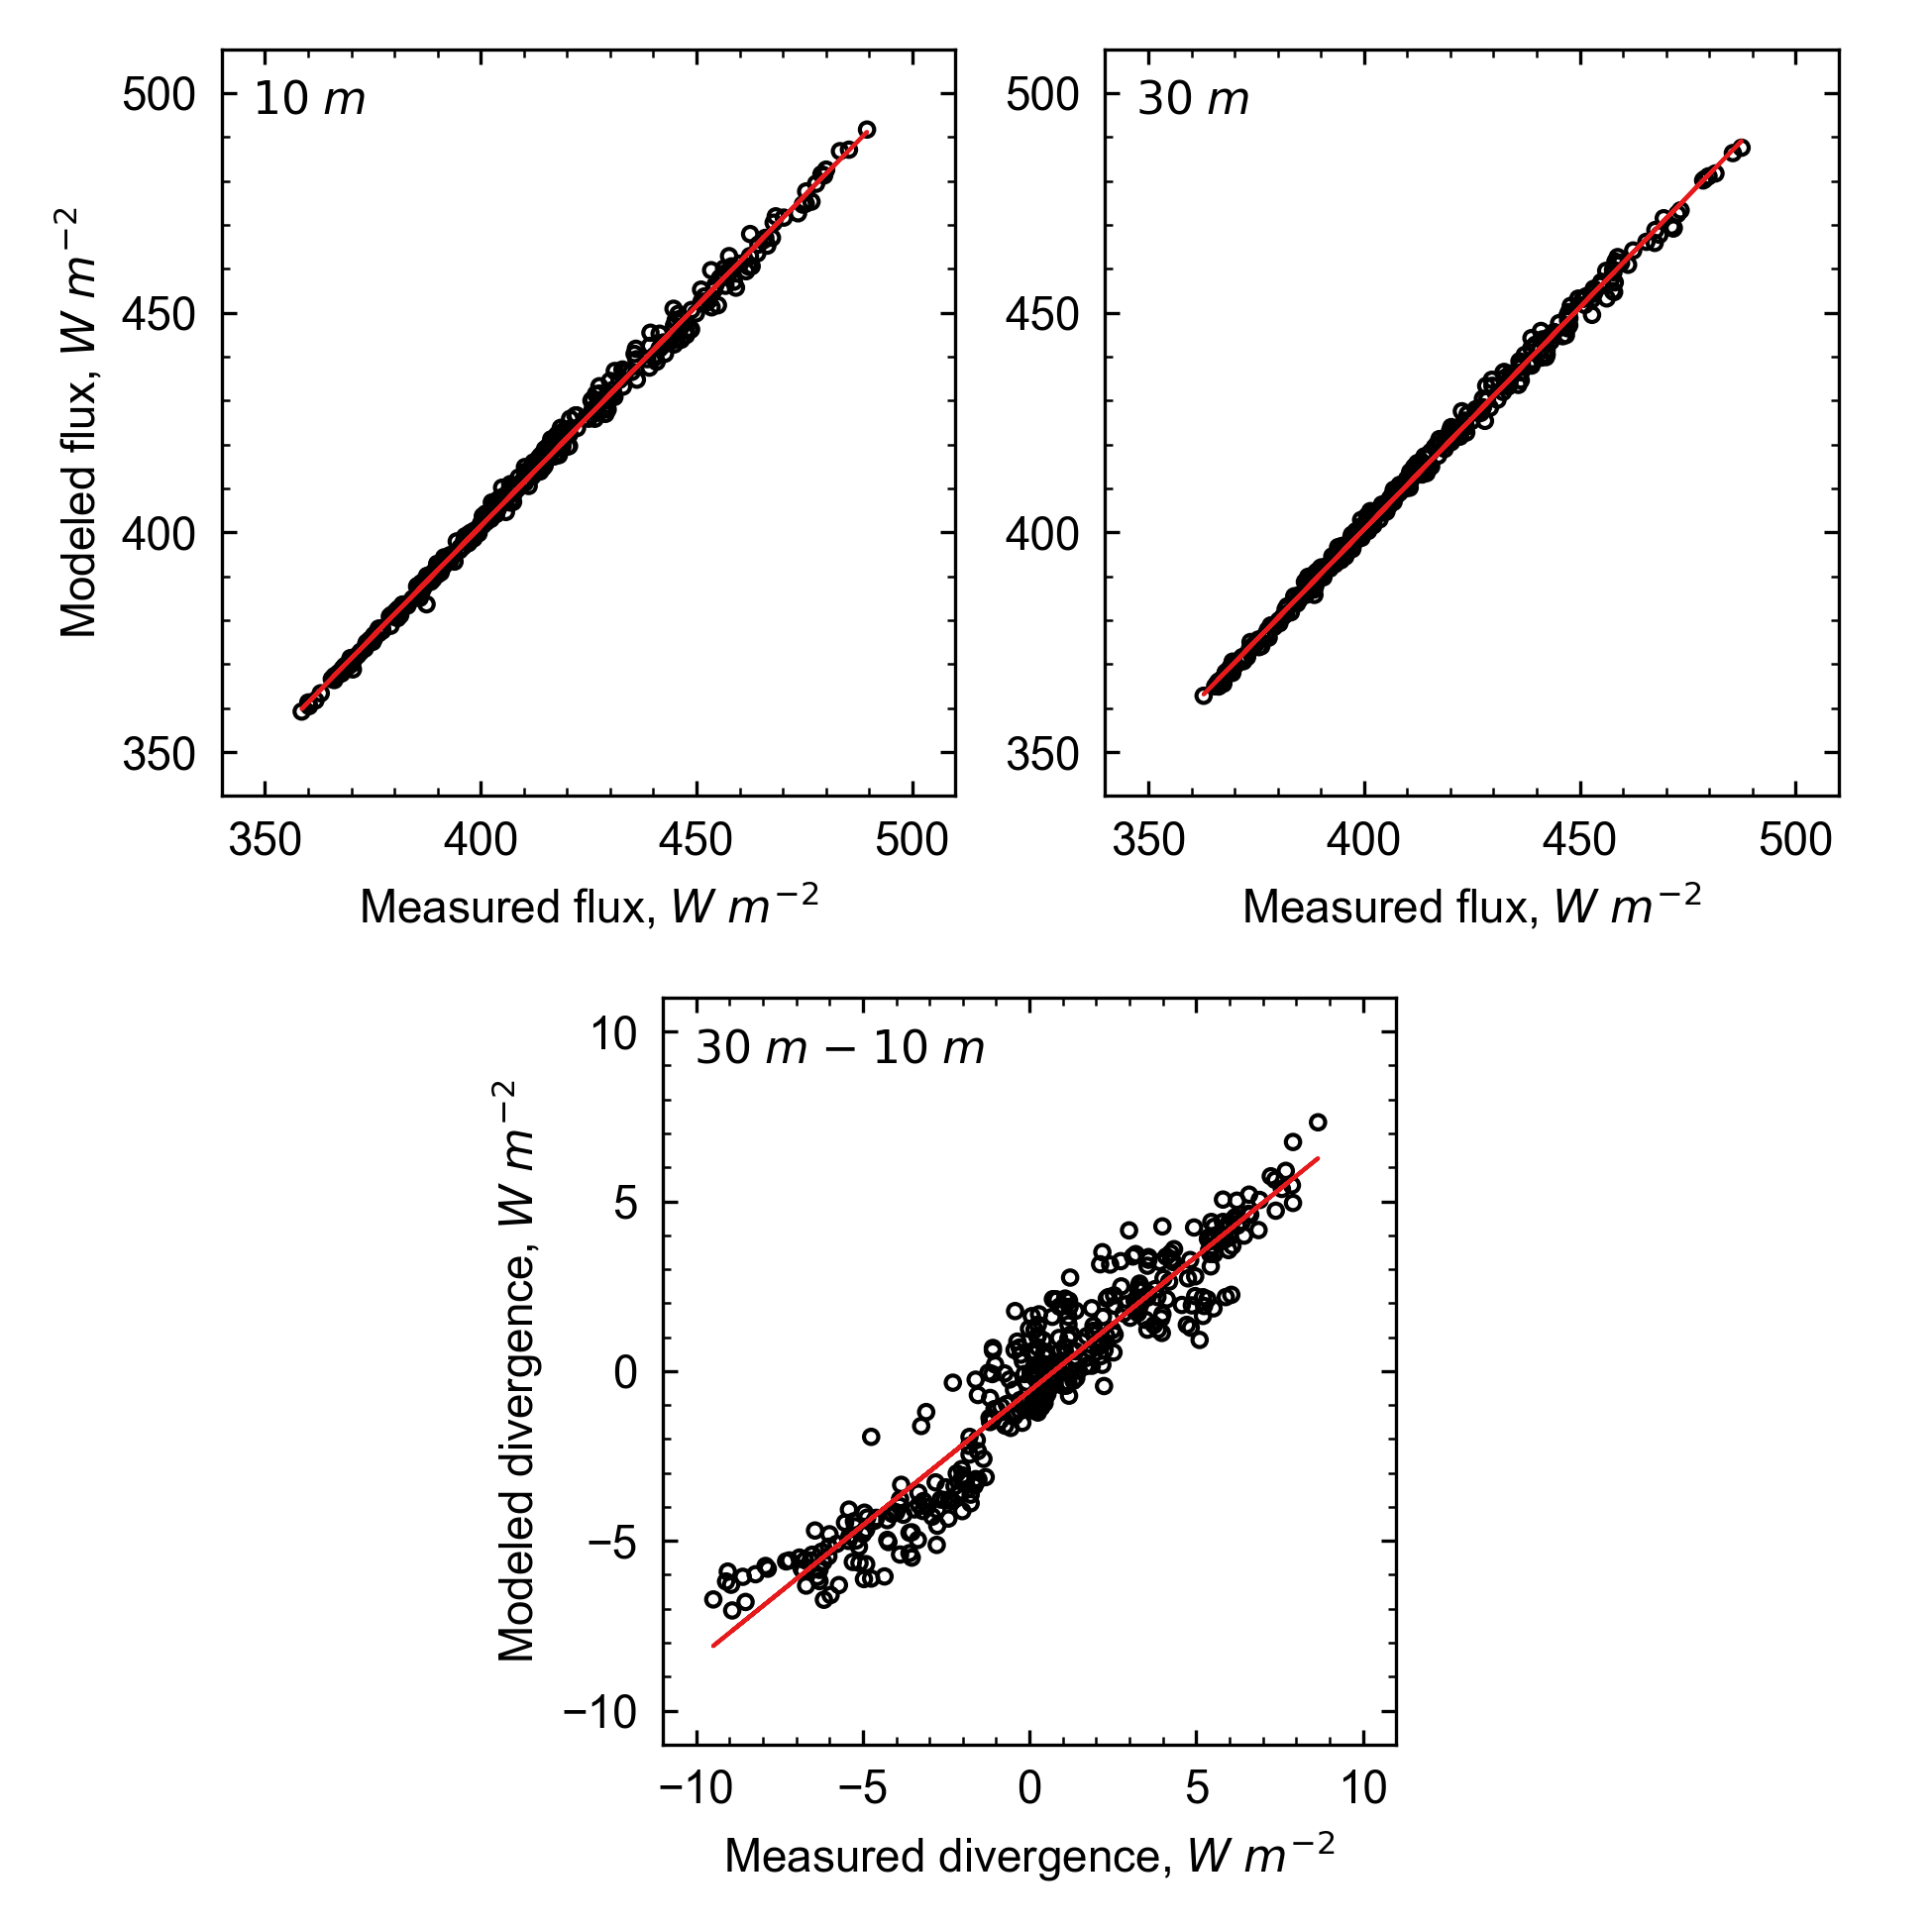
\includegraphics[width=\textwidth]{eval}
	\caption{A comparison of 10 \si{m} and 30 \si{m} measured and modeled longwave fluxes and divergences - calculated as the difference between 30 \si{\meter} and 10 \si{\meter} fluxes - over the 14 day evaluation period at Payerne, Switzerland.}
	\label{fluxes}
\end{figure}

\begin{table}[H]
	\centering
	\caption{Statistical performance of the Payerne evaluation. RMSE\textit{\textsubscript{s}} and RMSE\textit{\textsubscript{u}} represent the systemic and unsystematic RMSE respectively. n = 378}
	\label{evalstats}
	\begin{tabular*}{\textwidth}{l@{\extracolsep{\fill}} cccr}
		\toprule 
		Statistic & 10 \si{\meter} flux & 30 \si{\meter} flux & Divergence & Citation \\  \midrule
		Slope & 1.002 & 1.011 & 0.792 &  \\ 
		Intercept, (\si{\watt\per\meter\squared}) & 0.422 & $-$3.560 & $-$0.583 &   \\ 
		\textit{R\textsuperscript{2}} & 0.995 & 0.996 & 0.863 & \\ 
		MAE,  (\si{\watt\per\meter\squared}) & 1.781 & 1.325 & 1.191 & \citep{Willmott1985a} \\ 
		RMSE,  (\si{\watt\per\meter\squared}) & 2.204 & 1.690 & 1.423 & \citep{Willmott1985a} \\ 
		RMSE\textit{\textsubscript{s}},  (\si{\watt\per\meter\squared}) & 1.444 & 0.851 & 1.028 & \citep{Willmott1985a} \\ 
		RMSE\textit{\textsubscript{u}},  (\si{\watt\per\meter\squared}) & 1.666 & 1.460 & 0.985 & \citep{Willmott1985a} \\ 
		\textit{d}, agreement index & 0.999 & 0.999 & 0.959 & \citep{Willmott2012} \\
		\bottomrule
	\end{tabular*} 
\end{table}

\section{Results}

\subsection{Atmospheric correction magnitudes}

Atmospheric correction magnitudes binned for season and time of day are shown in Figure \ref{bx_ac}. Summertime correction magnitudes show significant day-to-day and diurnal variation. Variance is largest in summer near solar noon, where different synoptic conditions can force correction magnitudes of up to $8$ \si{\kelvin} in clear-sky hot conditions and below $0$ \si{\kelvin} under cooler overcast conditions. In winter, correction magnitudes display less variance and are smaller - approximately $2$ \si{\kelvin} over a range of representative wintertime synoptic conditions. 

Over both summer and winter seasons, correction magnitudes are strongly correlated with $\Delta$T\textsubscript{hem, r - air}. Figures \ref{season_sw} and \ref{season_sc} show the effect of seasonality and cloud cover on the relationship between correction magnitudes and $\Delta$T\textsubscript{hem, r - air}. The relationship is strongest and most evident in summer when variations in cloud cover can lead to large day-to-day contrasts in solar input and $\Delta$T\textsubscript{surf - air}, which translates into a wide range of correction magnitudes.

Figures \ref{meteo_k_hem} and \ref{meteo_air_hum}
 illustrate the relationship between correction magnitude and meteorological variables commonly measured as a part of climatological assessments of urban environments. A strong positive relationship is observed between correction magnitudes and incoming solar radiation. T\textsubscript{hem, r} and T\textsubscript{air} display more complex relationships with correction magnitude, with a large cluster of observed correction magnitudes situated at a local minimum between $10$ and $20$ \si{\degreeCelsius}, weakly negative correlation at temperatures lower than $10$ \si{\degreeCelsius}, and weakly positive correlation at temperatures greater than $20$ \si{\degreeCelsius}. Atmospheric water vapor content did not appear to exert significant control over correction magnitudes.

Figure \ref{humtest} shows hemispherical atmospheric transmittance as a function of vapor pressure for pyrgeometers at 10 \si{\meter} and 30 \si{\meter} above a flat surface. Transmittances are modeled in MODTRAN 4.1 as the fraction of surface emission reaching the sensor for the path length and view factor geometries calculated in the method evaluation in Section \ref{sensitivity}. Hemispherical transmittance falls sharply with increasing vapor pressure between 0 and 5 \si{\hecto\pascal}, but is relatively constant with vapor pressure \textgreater 5 \si{\hecto\pascal}. This results in the weak correlation observed in Figure \ref{meteo_air_hum} between humidity and correction magnitude.

%Correction magnitudes are most strongly dependent on incoming solar radiation - which exerts significant control over seasonal and diurnal variance in the T\textsubscript{hem, r} - T\textsubscript{air} differential. These observations are largely made up of nighttime and cloudy points during the summer months with small or weakly negative T\textsubscript{surf} - T\textsubscript{air} differentials. During the winter months, a negative relationship between T\textsubscript{hem, r}/T\textsubscript{air} and correction magnitudes is observed at lower overall T\textsubscript{hem, r} and T\textsubscript{air}. In summer months, a positive relationship between T\textsubscript{hem, r}/T\textsubscript{air} and correction magnitudes is observed at higher overall temperatures. 

\begin{figure}[H]
	\centering
	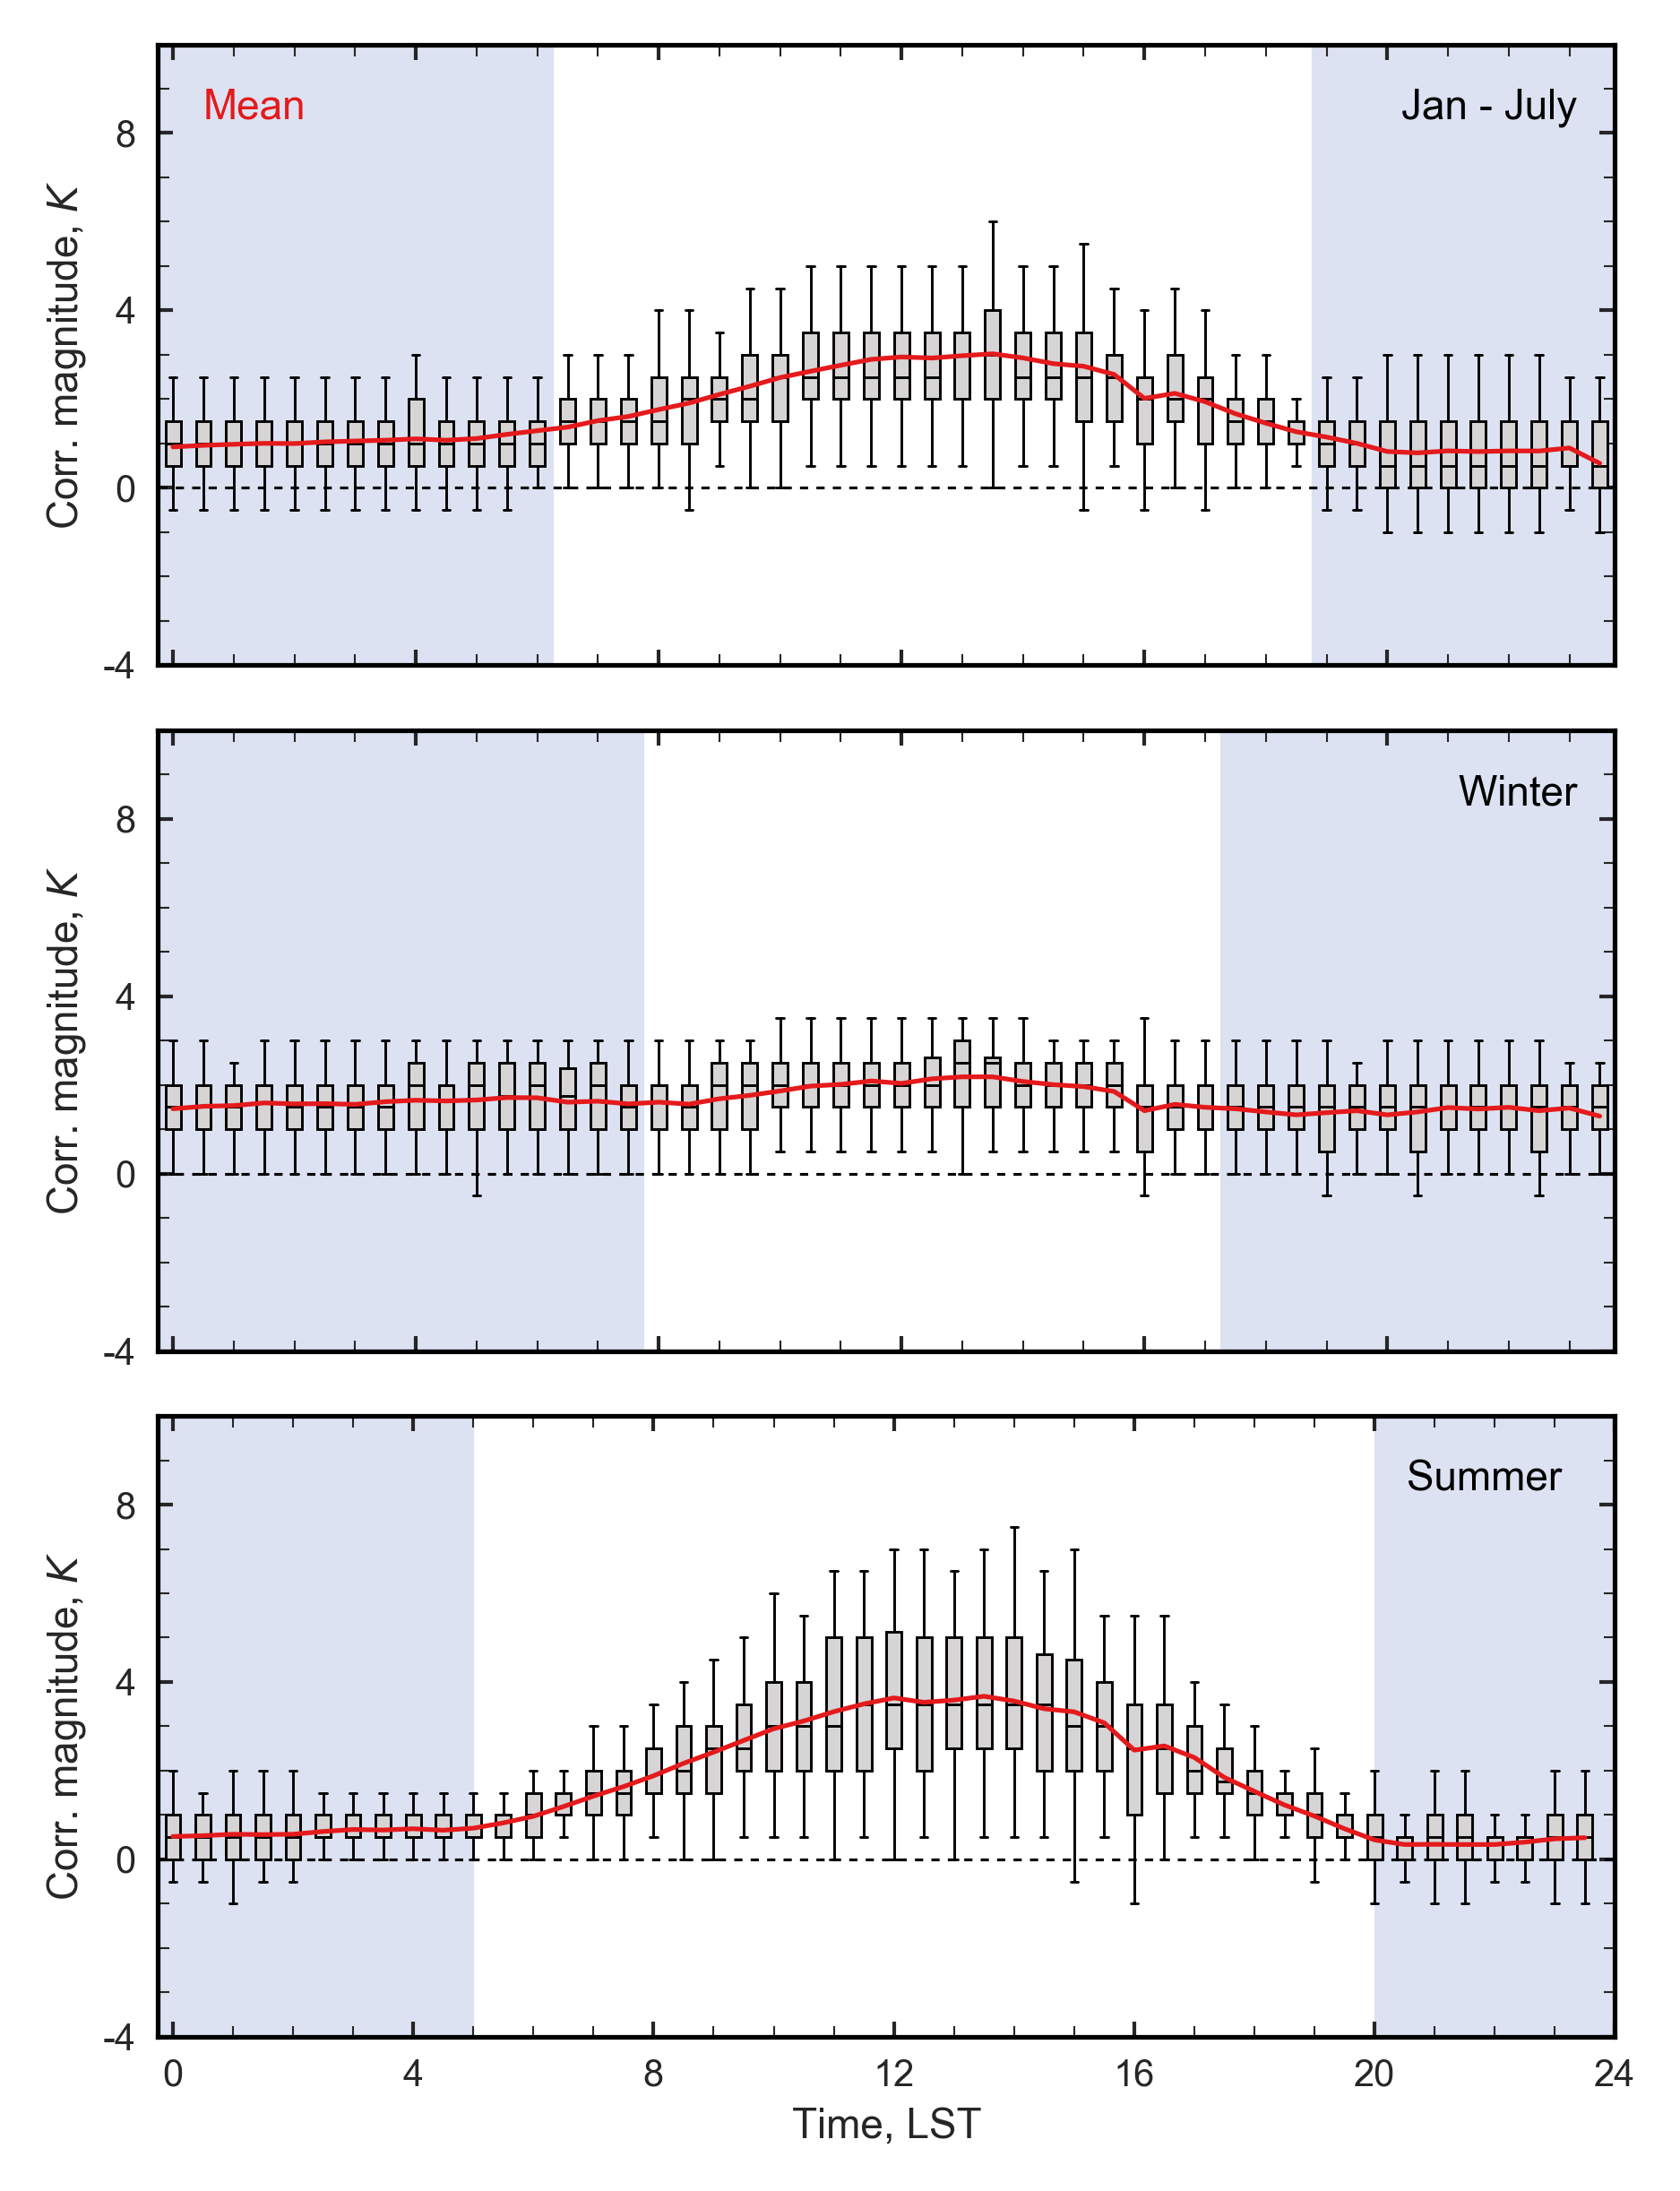
\includegraphics[width=15cm,
	height=7in,
	keepaspectratio]{bx_ac1}
	\caption{Atmospheric correction magnitudes calculated as the difference between T\textsubscript{hem, r} and T\textsubscript{hem, b} for the duration of the study period. Grey shading indicates nighttime. The red line indicates mean correction magnitude at each time step.}
	\label{bx_ac}
\end{figure}

\begin{figure}[H]
	\centering
	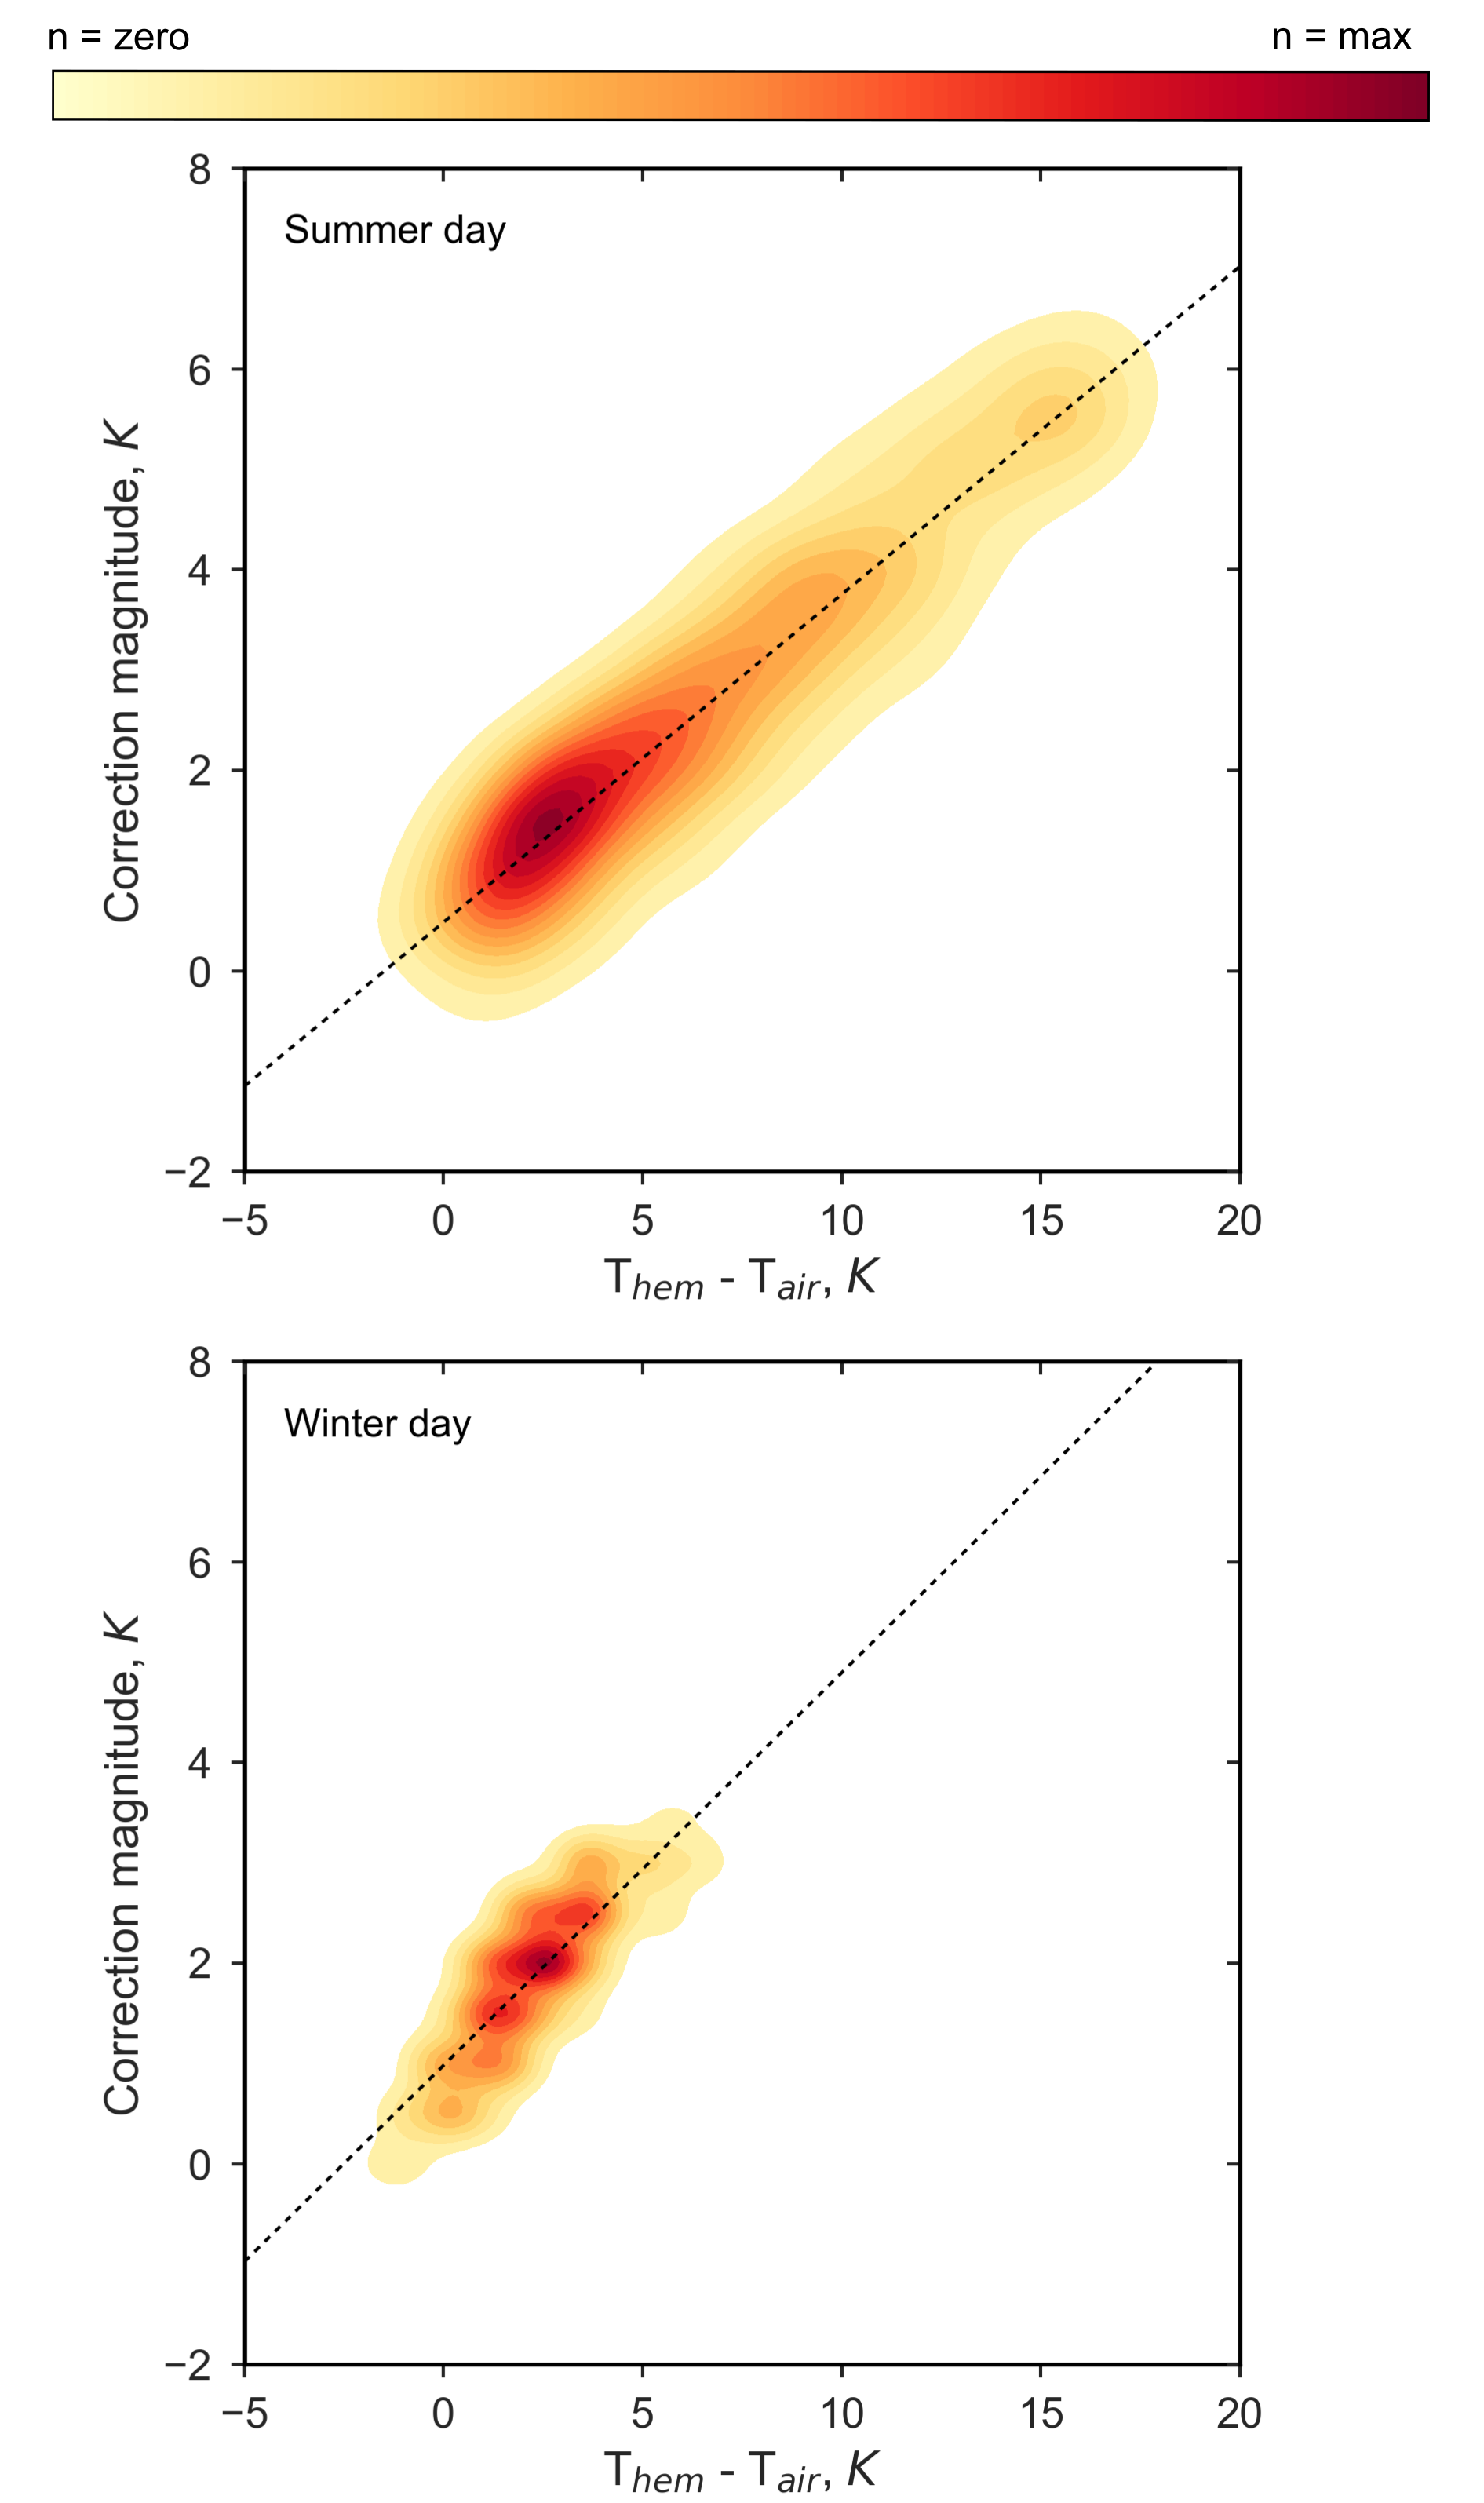
\includegraphics[width=15cm,
	height=7in,
	keepaspectratio]{season_sw}
	\caption{Correction magnitude versus $\Delta$T\textsubscript{hem, r - air} binned for season.}
	\label{season_sw}
\end{figure}

\begin{figure}[H]
	\centering
	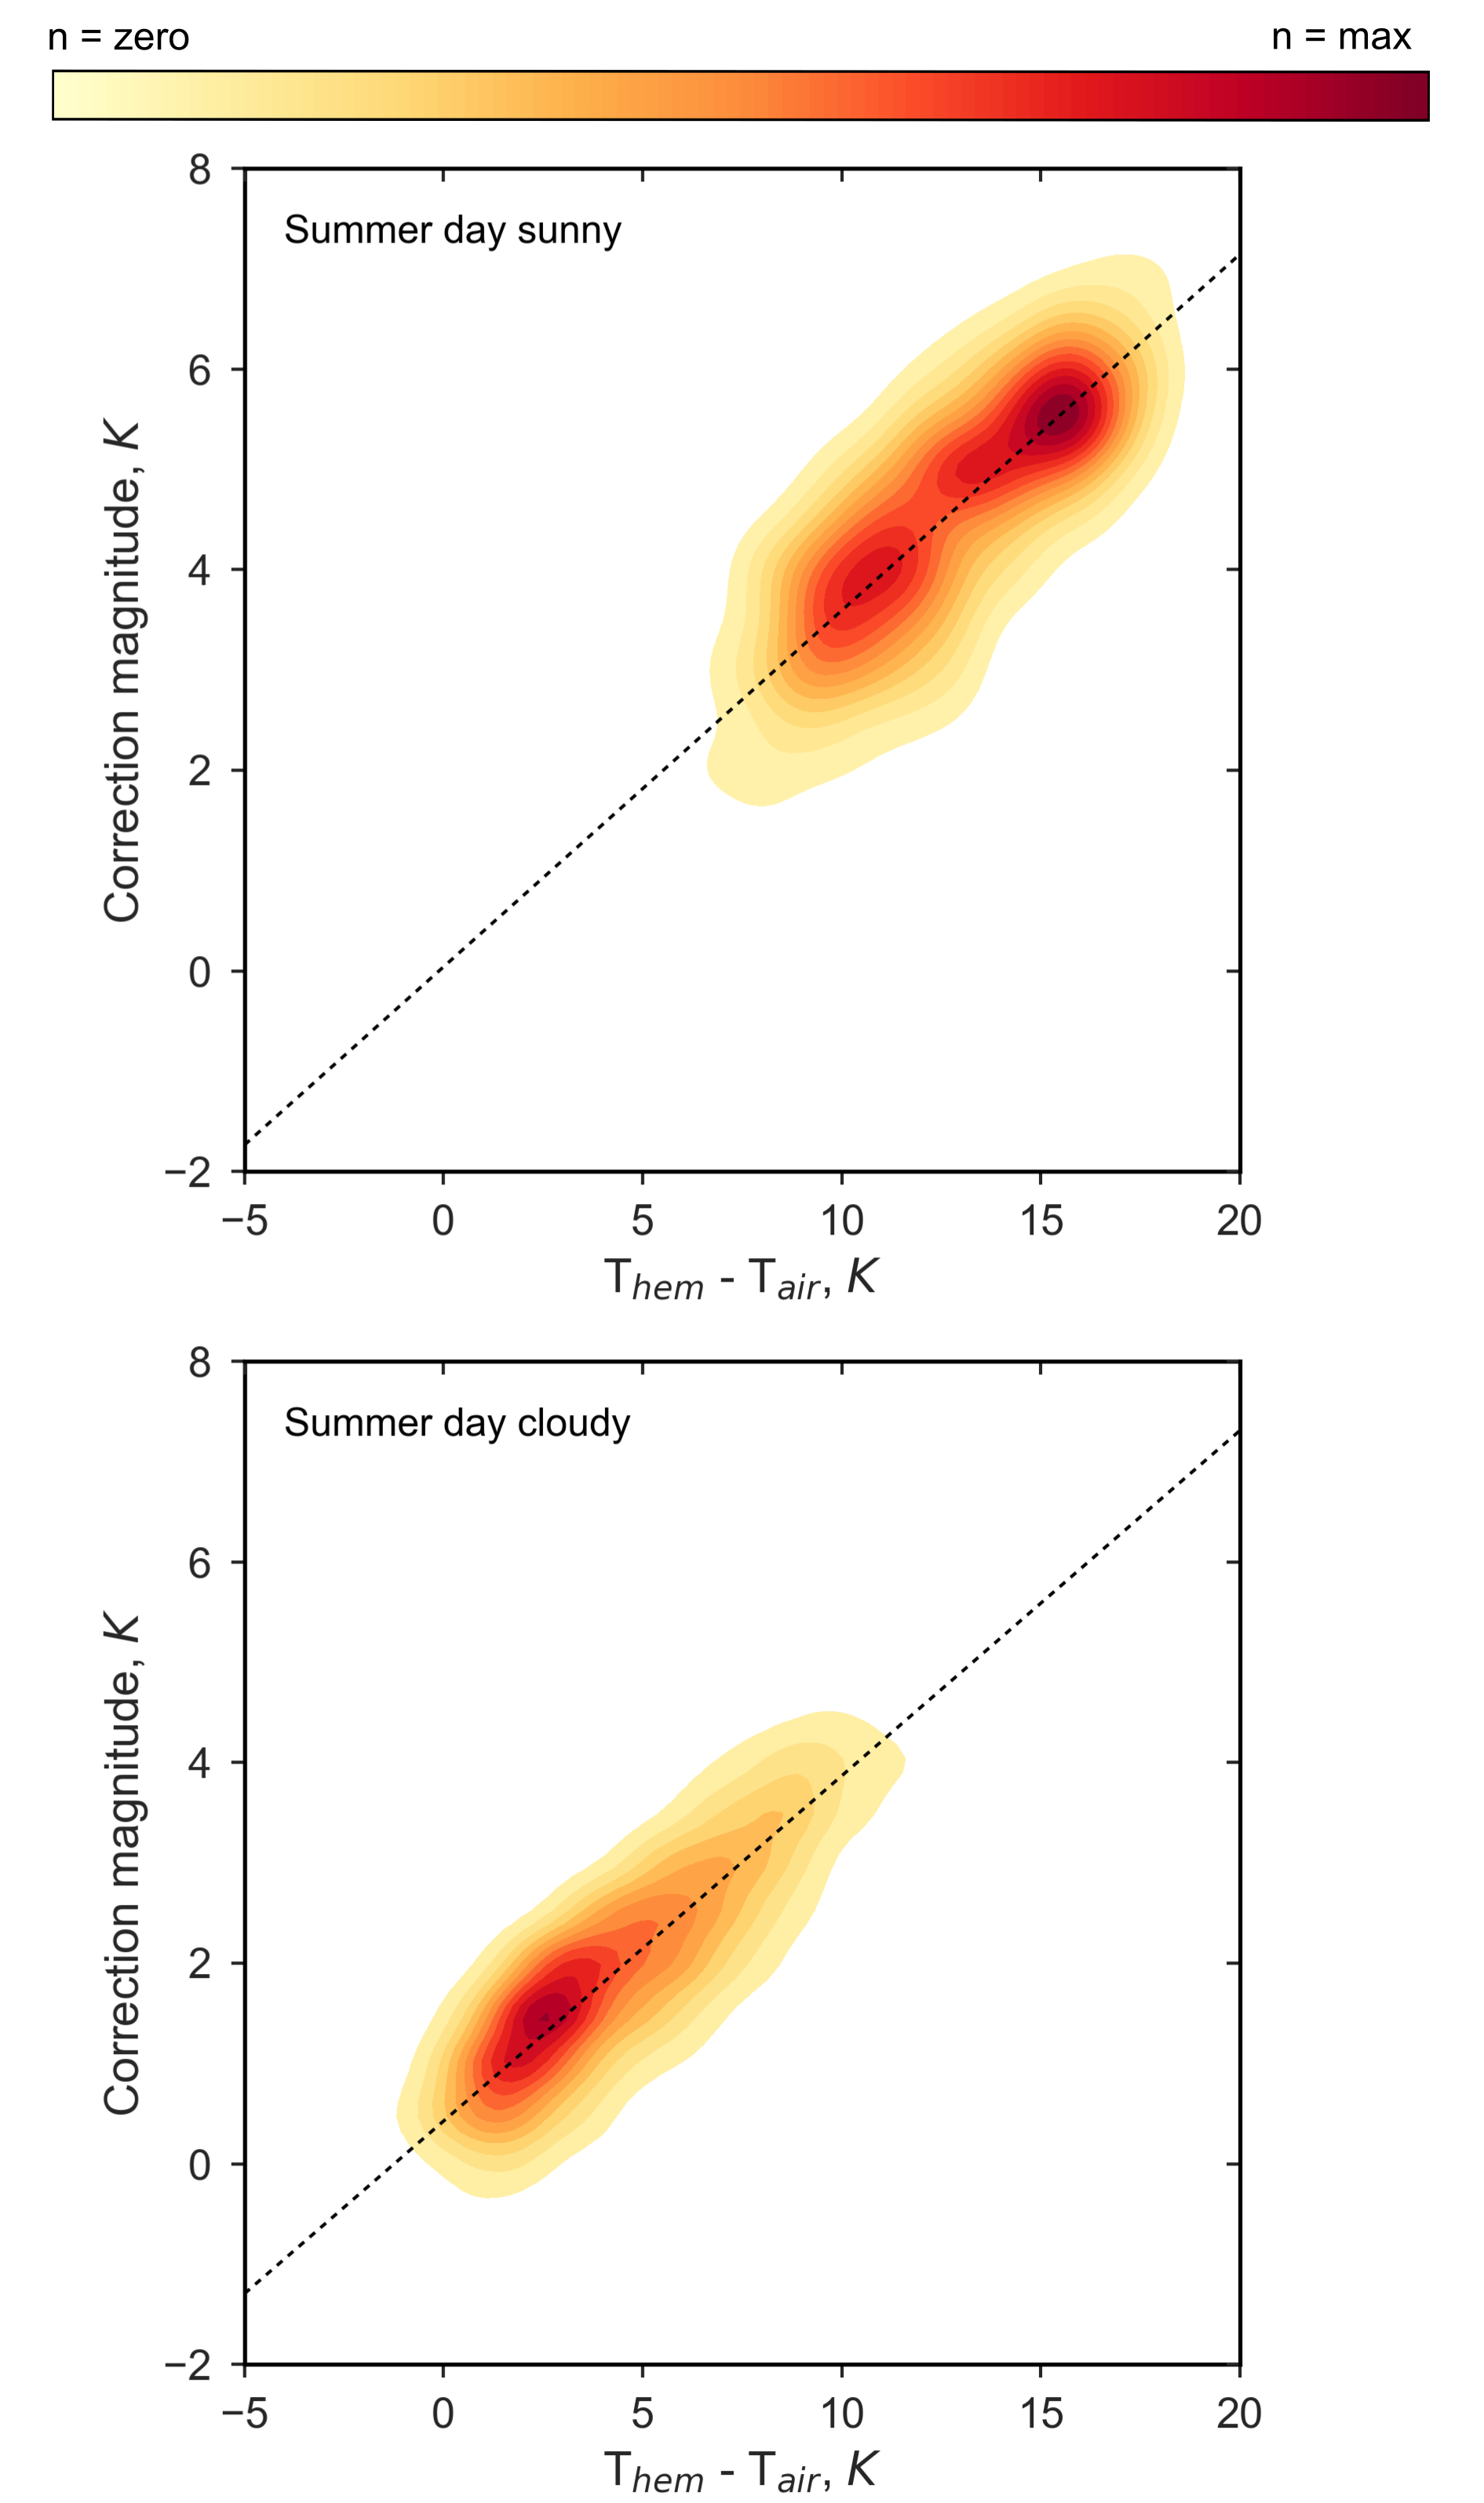
\includegraphics[width=15cm,
	height=7in,
	keepaspectratio]{season_sc}
	\caption{Correction magnitude versus $\Delta$T\textsubscript{hem, r - air} binned for clear and clouded days over the summer months.}
	\label{season_sc}
\end{figure}

\begin{figure}[H]
	\centering
	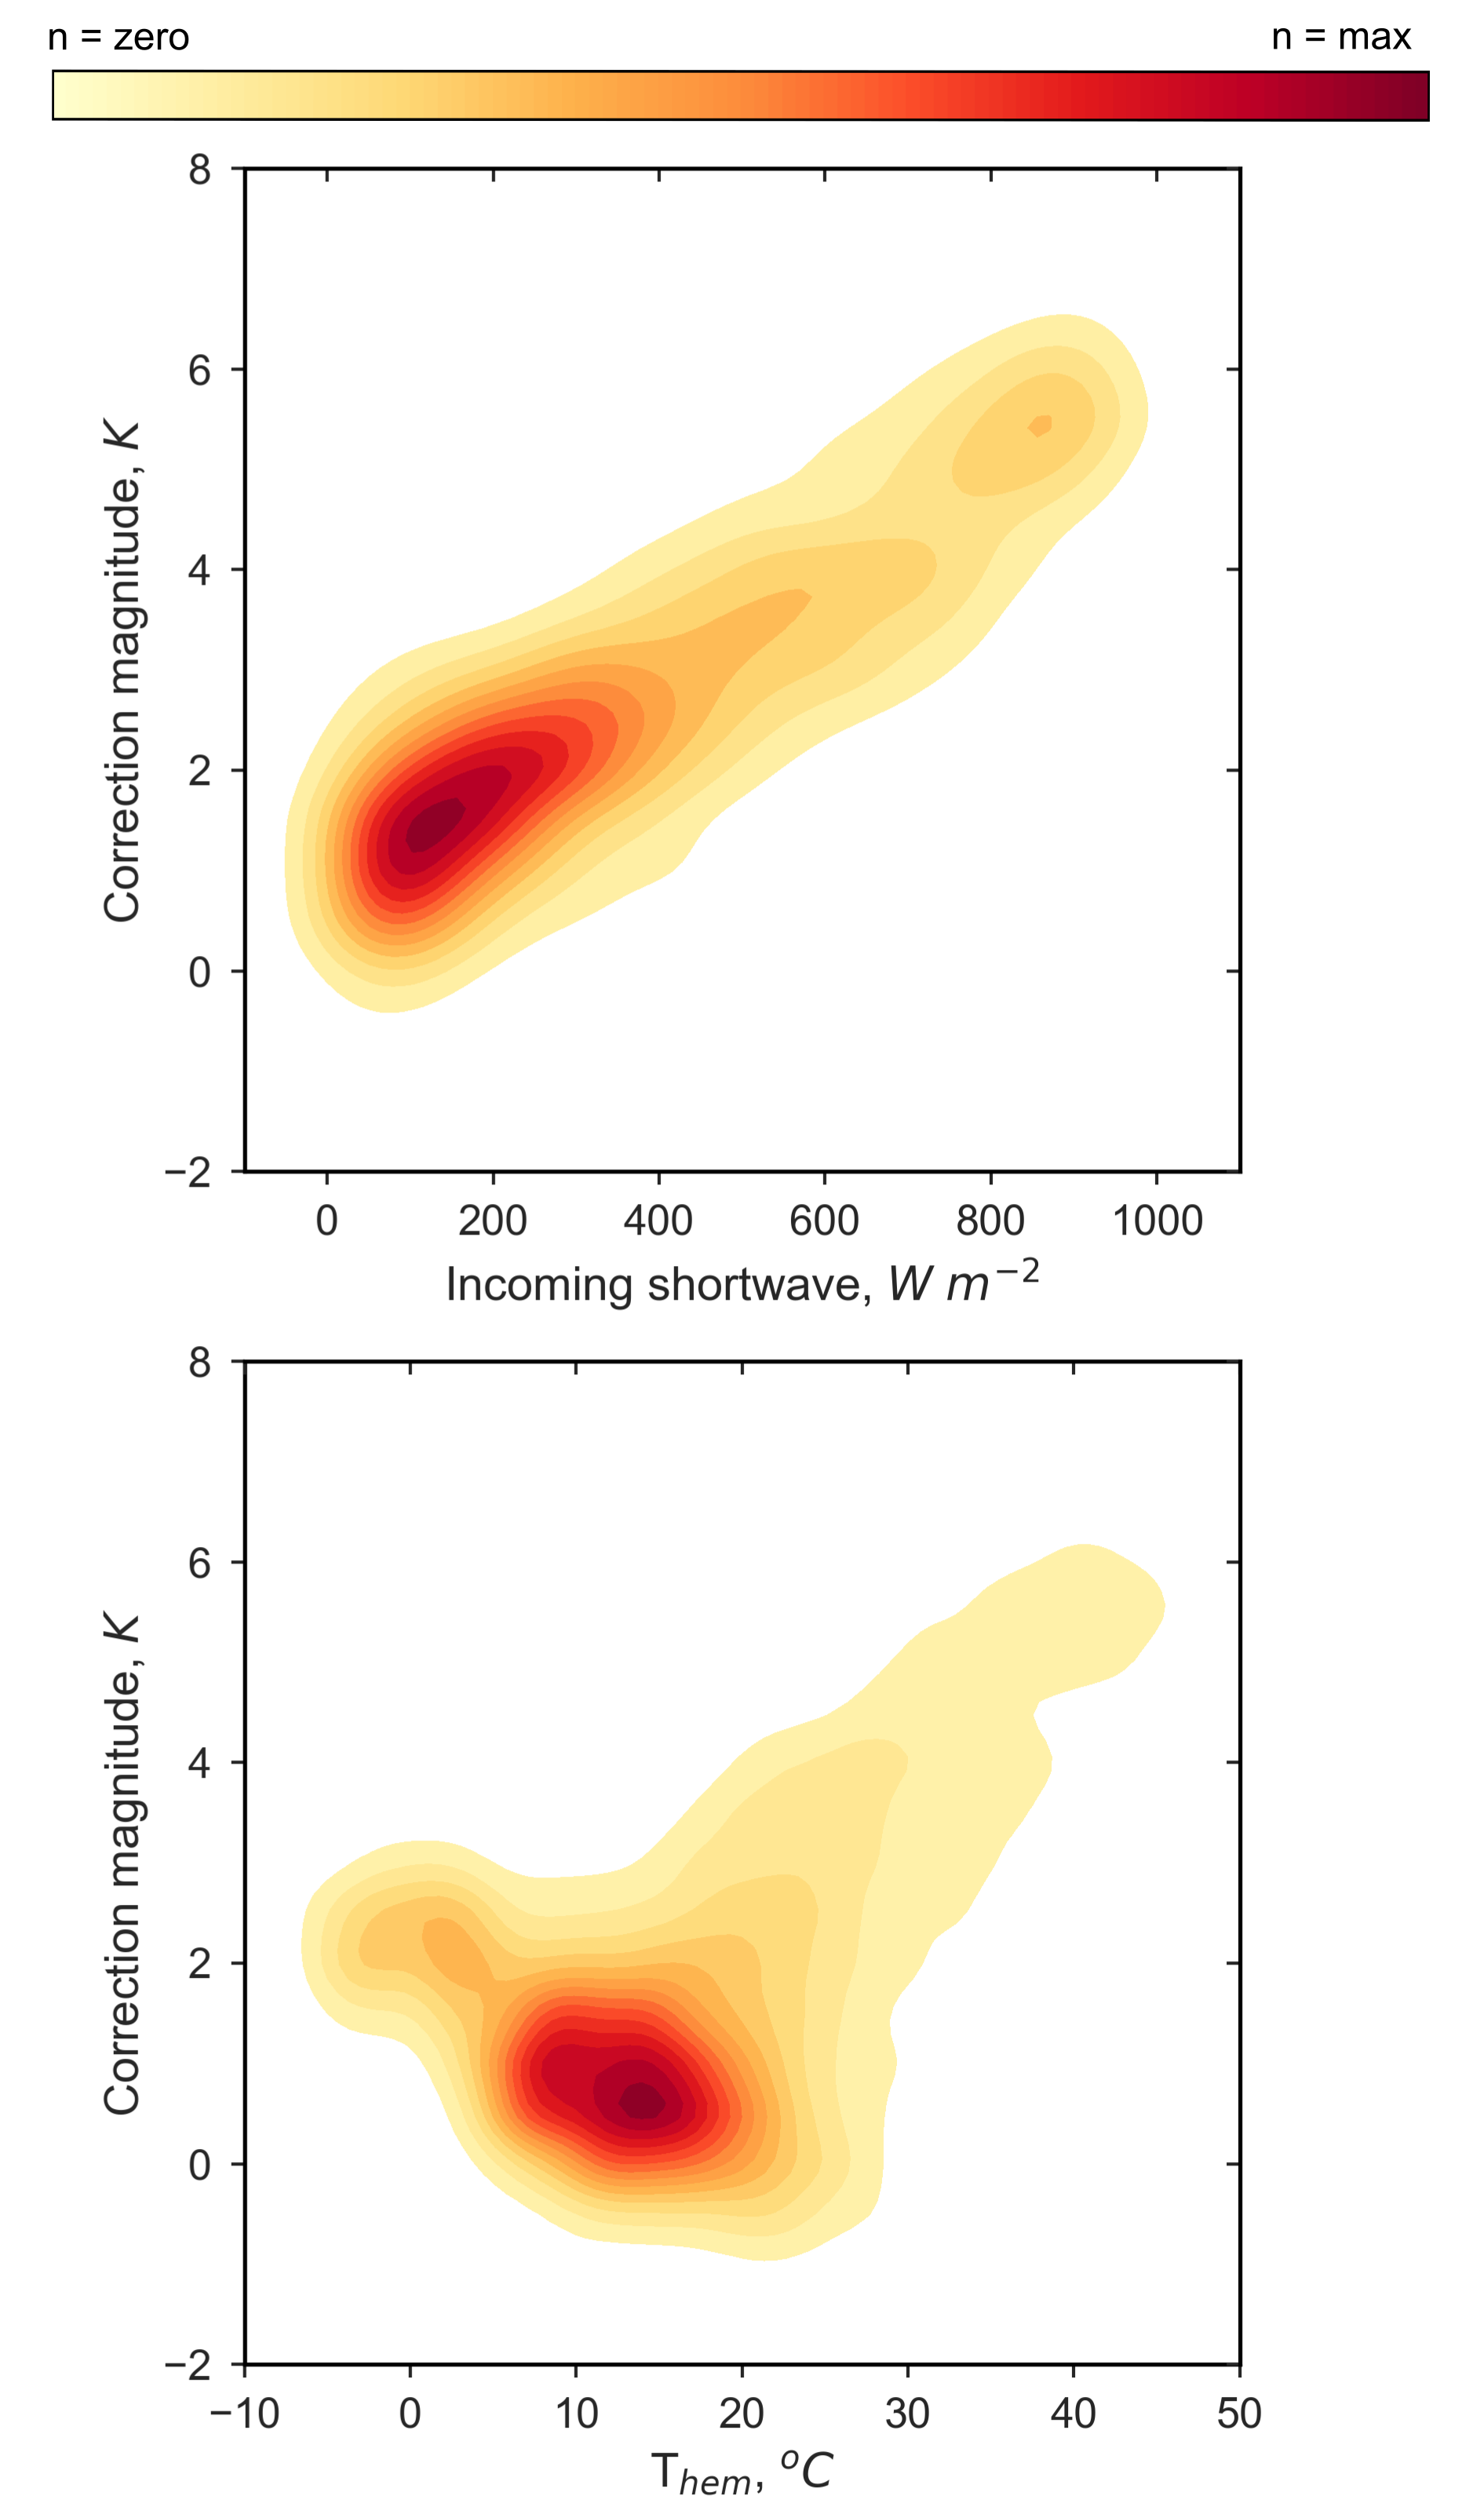
\includegraphics[width=15cm,
	height=7in,
	keepaspectratio]{meteo_k_hem}
	\caption{Correction magnitude versus incoming shortwave and T\textsubscript{hem, r} for the daytime hours of the study period.}
	\label{meteo_k_hem}
\end{figure}

\begin{figure}[H]
	\centering
	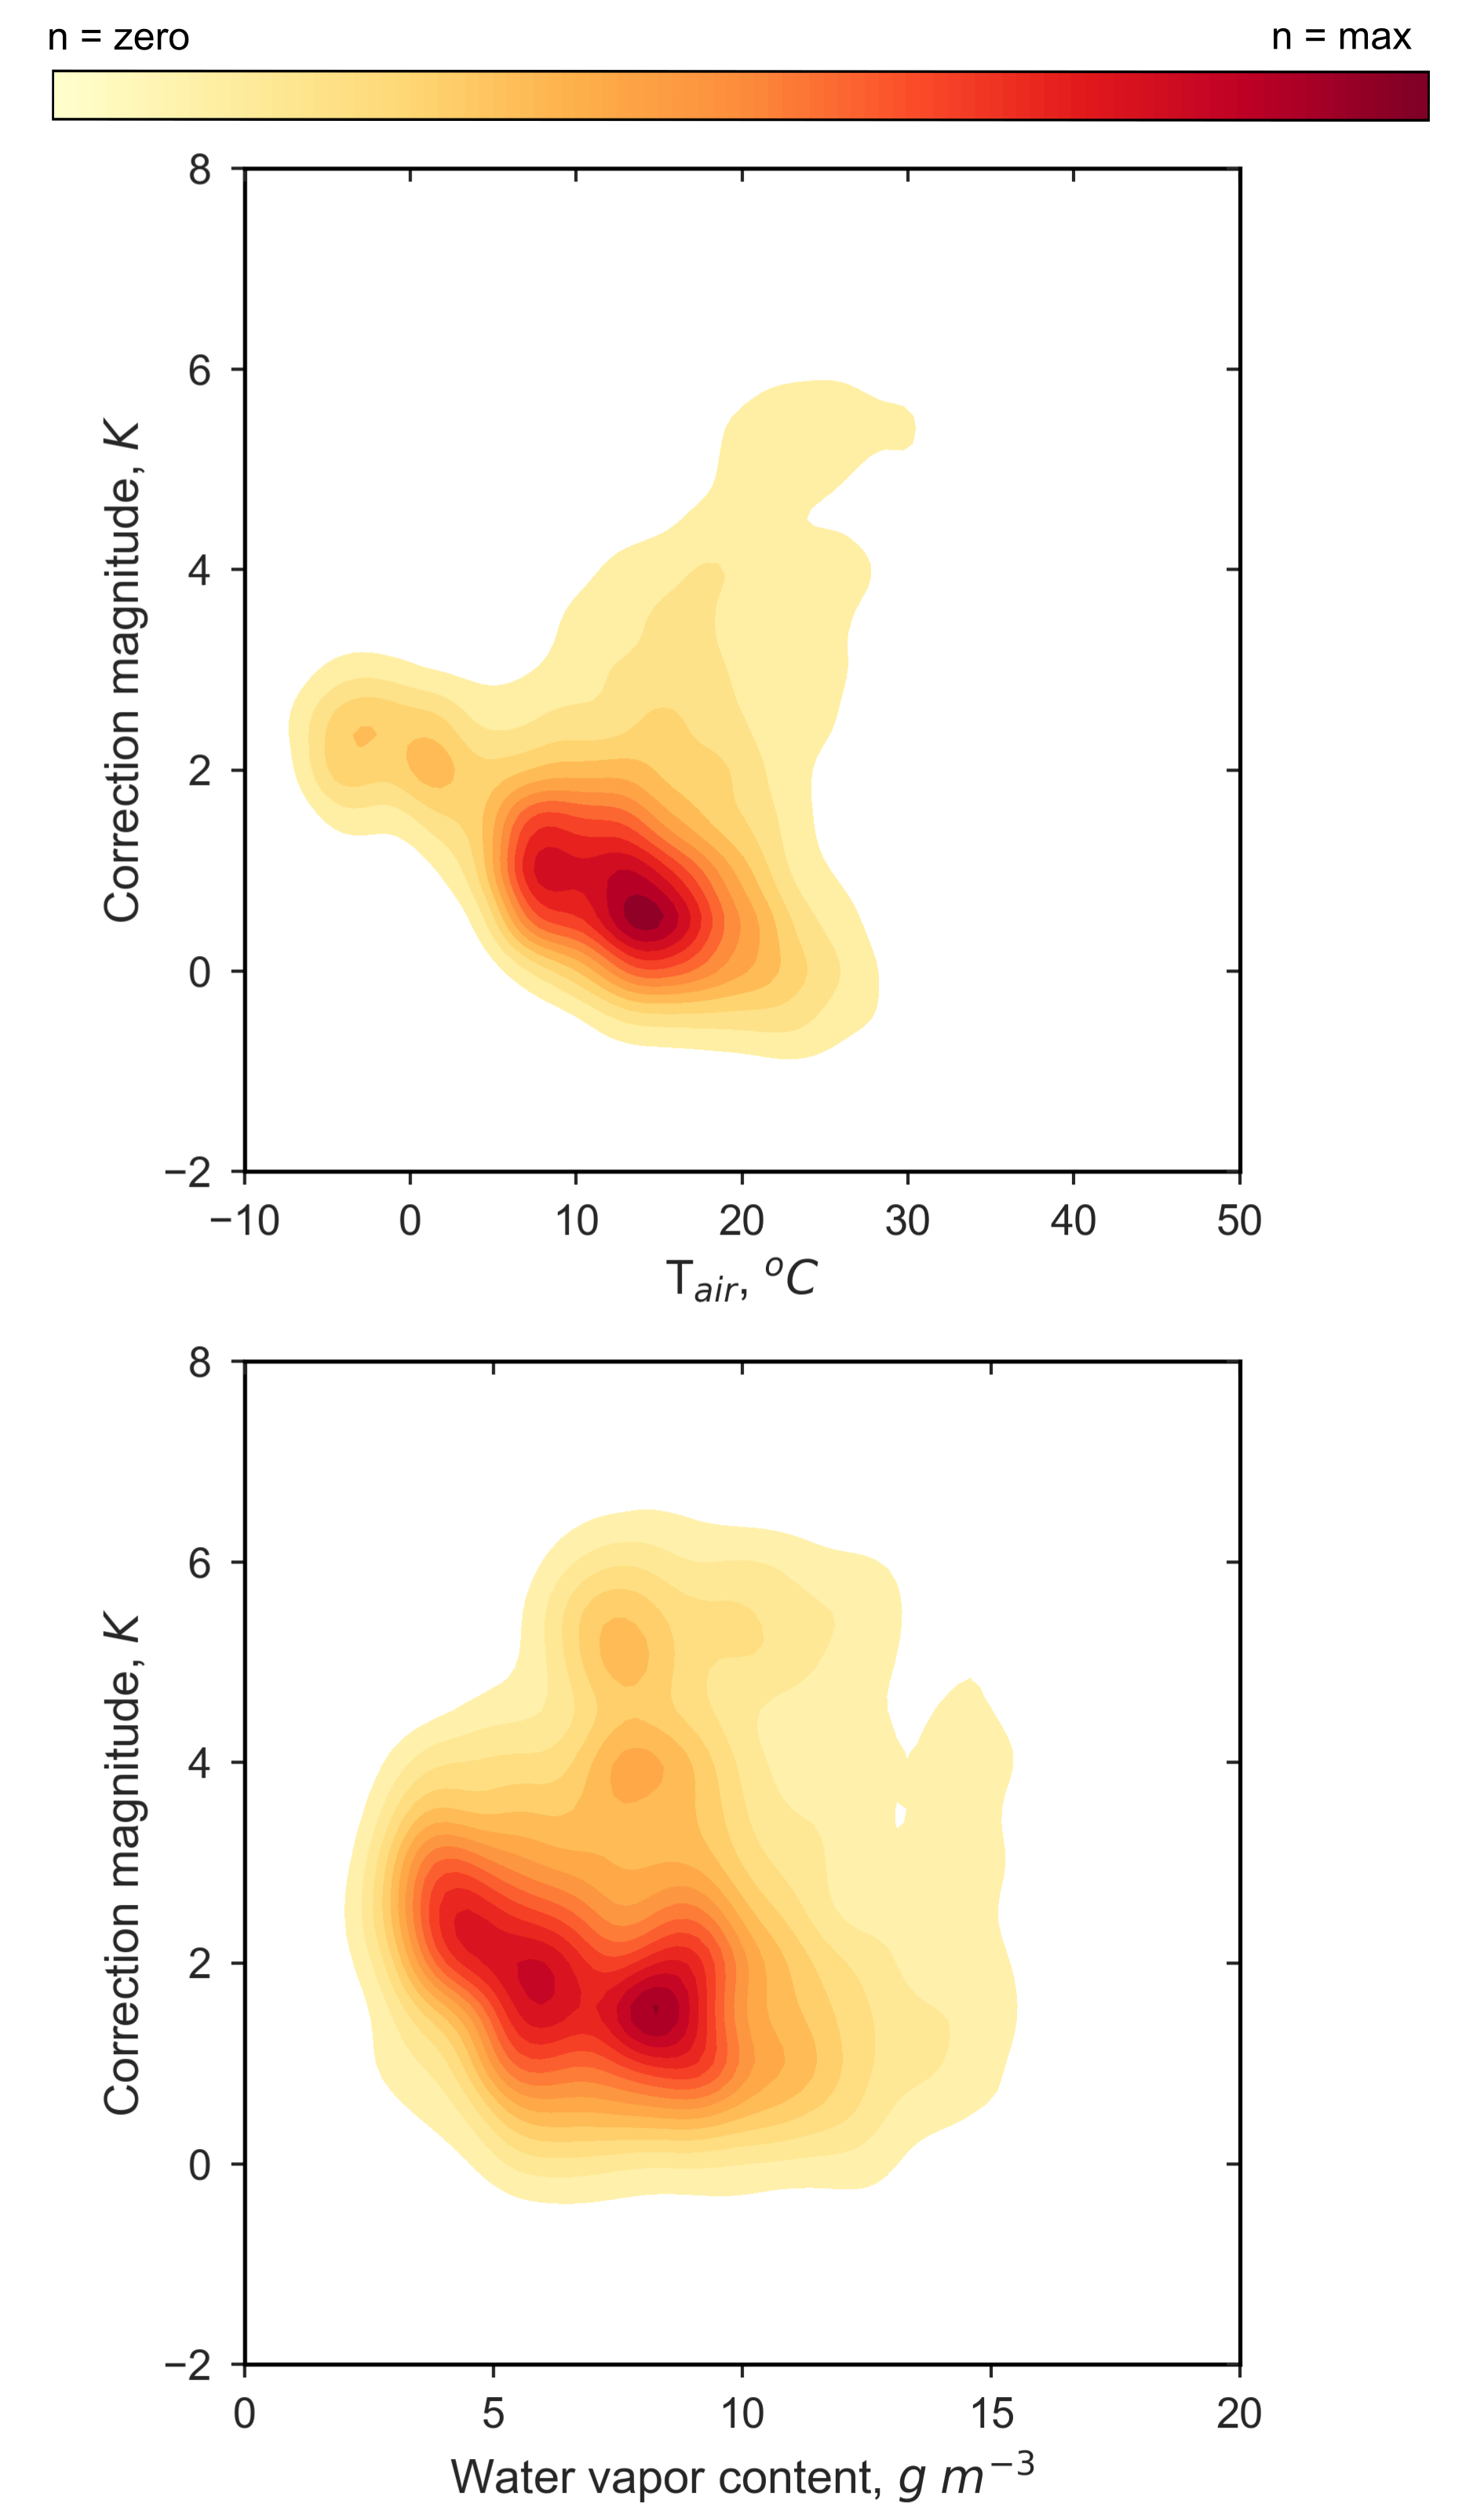
\includegraphics[width=15cm,
	height=7in,
	keepaspectratio]{meteo_air_hum}
	\caption{Correction magnitude versus T\textsubscript{air} and water vapor content for the daytime hours of the study period.}
	\label{meteo_air_hum}
\end{figure}

\begin{figure}[H]
	\centering
	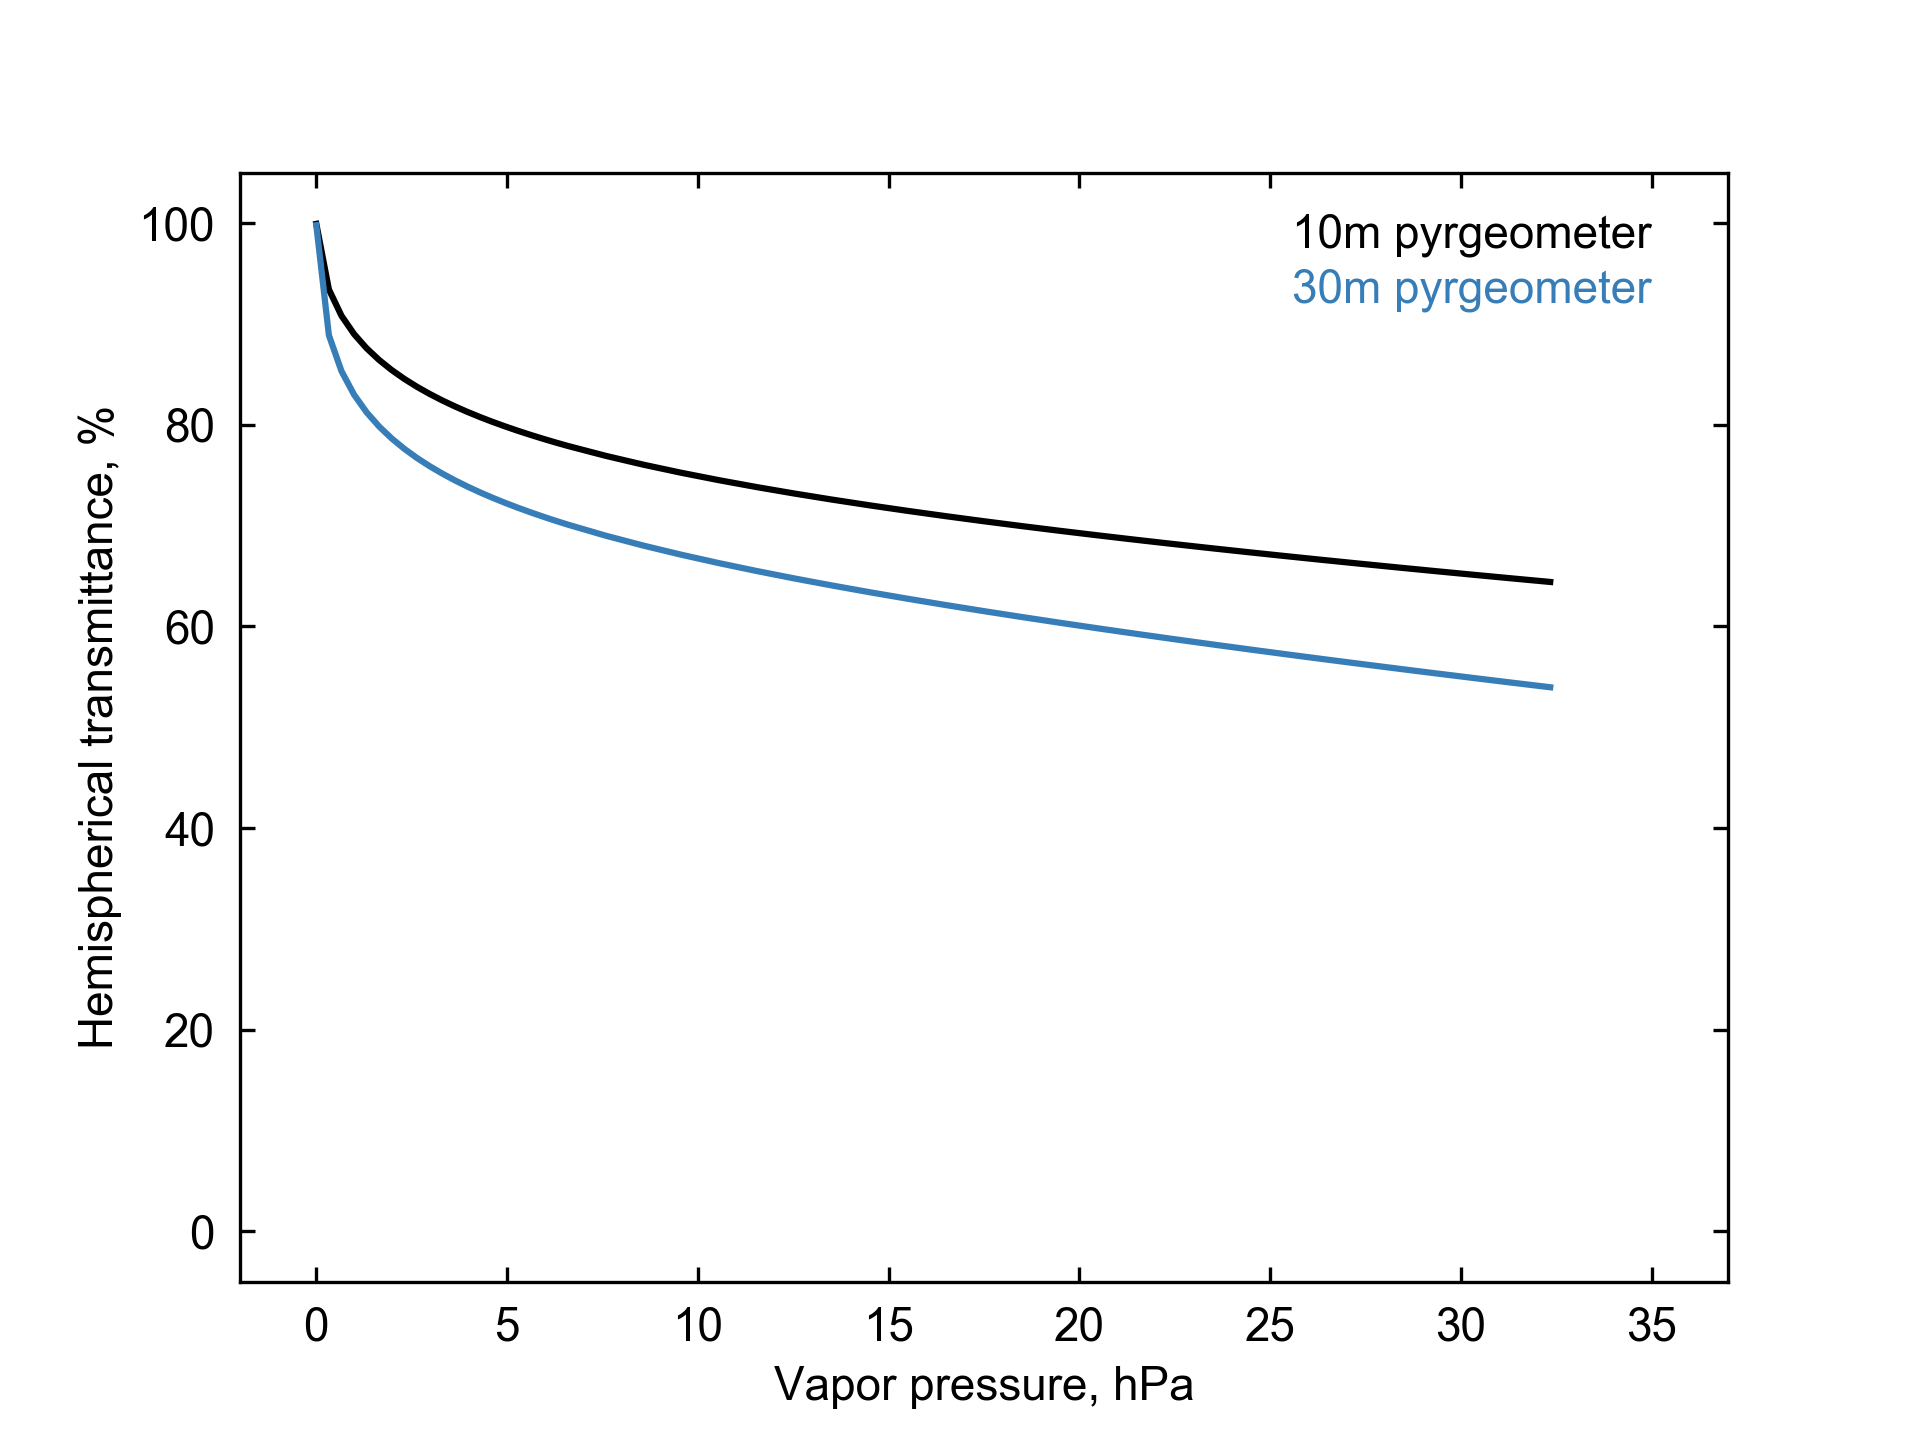
\includegraphics[width=15cm,
	height=7in,
	keepaspectratio]{hum_test}
	\caption{Hemispherical at-sensor atmospheric transmittance as a function of vapor pressure for two pyrgeometer heights (10 \si{\meter} and 30 \si{\meter}) over a flat surface. Calculated as the fraction of surface emission reaching the sensor height using MODTRAN 4.1 with T\textsubscript{surf} = T\textsubscript{air} = 300 \si{\kelvin} with water vapor as the sole atmospheric absorber.}
	\label{humtest}
\end{figure}

%\subsection{Relating correction magnitudes to climatological parameters}

%Correction magnitudes show strong diurnal and seasonal relationships with the T\textsubscript{surf} - T\textsubscript{air} differential - shown in figure \ref{season_fit}. As such, parameters that determine the T\textsubscript{surf} - T\textsubscript{air} differential exert similar control over correction magnitudes, most notably incoming shortwave radiation, T\textsubscript{surf}, and T\textsubscript{air}, shown in figures \ref{nofit}. Correction magnitudes are greatest with large shortwave radiation input and with high T\textsubscript{air} and T\textsubscript{hem, r}, during which contrasts between T\textsubscript{air} and T\textsubscript{surf} are largest. Conversely, correction magnitudes are smallest under conditions that suppress contrasts between T\textsubscript{surf} and T\textsubscript{air} - when solar input is small, and with low T\textsubscript{air} and T\textsubscript{hem, r}. In summer, variations in solar input based on time of day and cloud cover produce large fluctuations in the T\textsubscript{surf} - T\textsubscript{air} differential and significant variation in correction magnitude with time of day and synoptic conditions. Thus, maximum correction magnitudes occur on hot, clear-sky days, when solar input, T\textsubscript{air} and T\textsubscript{hem, r} are also maximized. Conversely, overcast and nighttime conditions with zero or low incoming solar radiation produce smaller or negative T\textsubscript{surf} - T\textsubscript{air} differentials and suppress correction magnitudes. In winter, a lower solar angle and shorter day length reduce overall solar input and the diurnal amplitude of T\textsubscript{hem, r} and T\textsubscript{air}. This suppresses both the overall size and diurnal amplitude of the T\textsubscript{surf} - T\textsubscript{air} differential and has a similar effect on winter correction magnitudes.

%Atmospheric transmittance of longwave radiation is primarily determined by column water vapor content. However, correction magnitudes are only weakly correlated with humidity (figure \ref{corr_abshum}). This supports the notion that atmospheric transmittance determines the \textit{potential} for atmospheric effects on a remote sensed TIR signal, but not necessarily the \textit{magnitude} of atmospheric influence. In the absence of a strong contrast between T\textsubscript{surf} and T\textsubscript{air}, absorption and reemission of TIR by water vapor or other absorbers has little effect on a remote sensed signal. Contra, with a strong contrast between T\textsubscript{surf} and T\textsubscript{air}, but little absorber content, the atmosphere is highly transmissive and does not yield strong atmospheric effects. 

\section{Comparing T\textsubscript{surf} from different sensor geometries}

To illustrate the effect of sensor-surface geometry on remote sensed T\textsubscript{surf}, Figure \ref{tc_nadhem} shows a comparison of mean normalized T\textsubscript{hem, r} and T\textsubscript{plan} calculated as T\textsubscript{x} divided by T\textsubscript{comp}, where T\textsubscript{x} is T\textsubscript{hem, r} or T\textsubscript{plan}, and averaged over the IOP. In the figure, overestimation of T\textsubscript{comp} is observed at values above one and underestimation by values below one. Both T\textsubscript{hem, r} and T\textsubscript{plan} overestimate T\textsubscript{comp} by day and underestimate T\textsubscript{comp} by night. Mean daytime overestimation of T\textsubscript{comp} by T\textsubscript{hem, r} is smaller and less variable than that by T\textsubscript{plan}. 

Mean normalized T\textsubscript{hem, r}, T\textsubscript{plan}, and $\Delta$T\textsubscript{plan - hem, r} are shown in Figure \ref{tc_mean2} along with clear sky and overcast sky case days. While mean T\textsubscript{hem, r} and T\textsubscript{plan} display similar overestimations of T\textsubscript{comp}, under clear sky conditions, overestimation by T\textsubscript{plan} is much larger than that by T\textsubscript{hem, r}.

\begin{figure}[H]
	\centering
	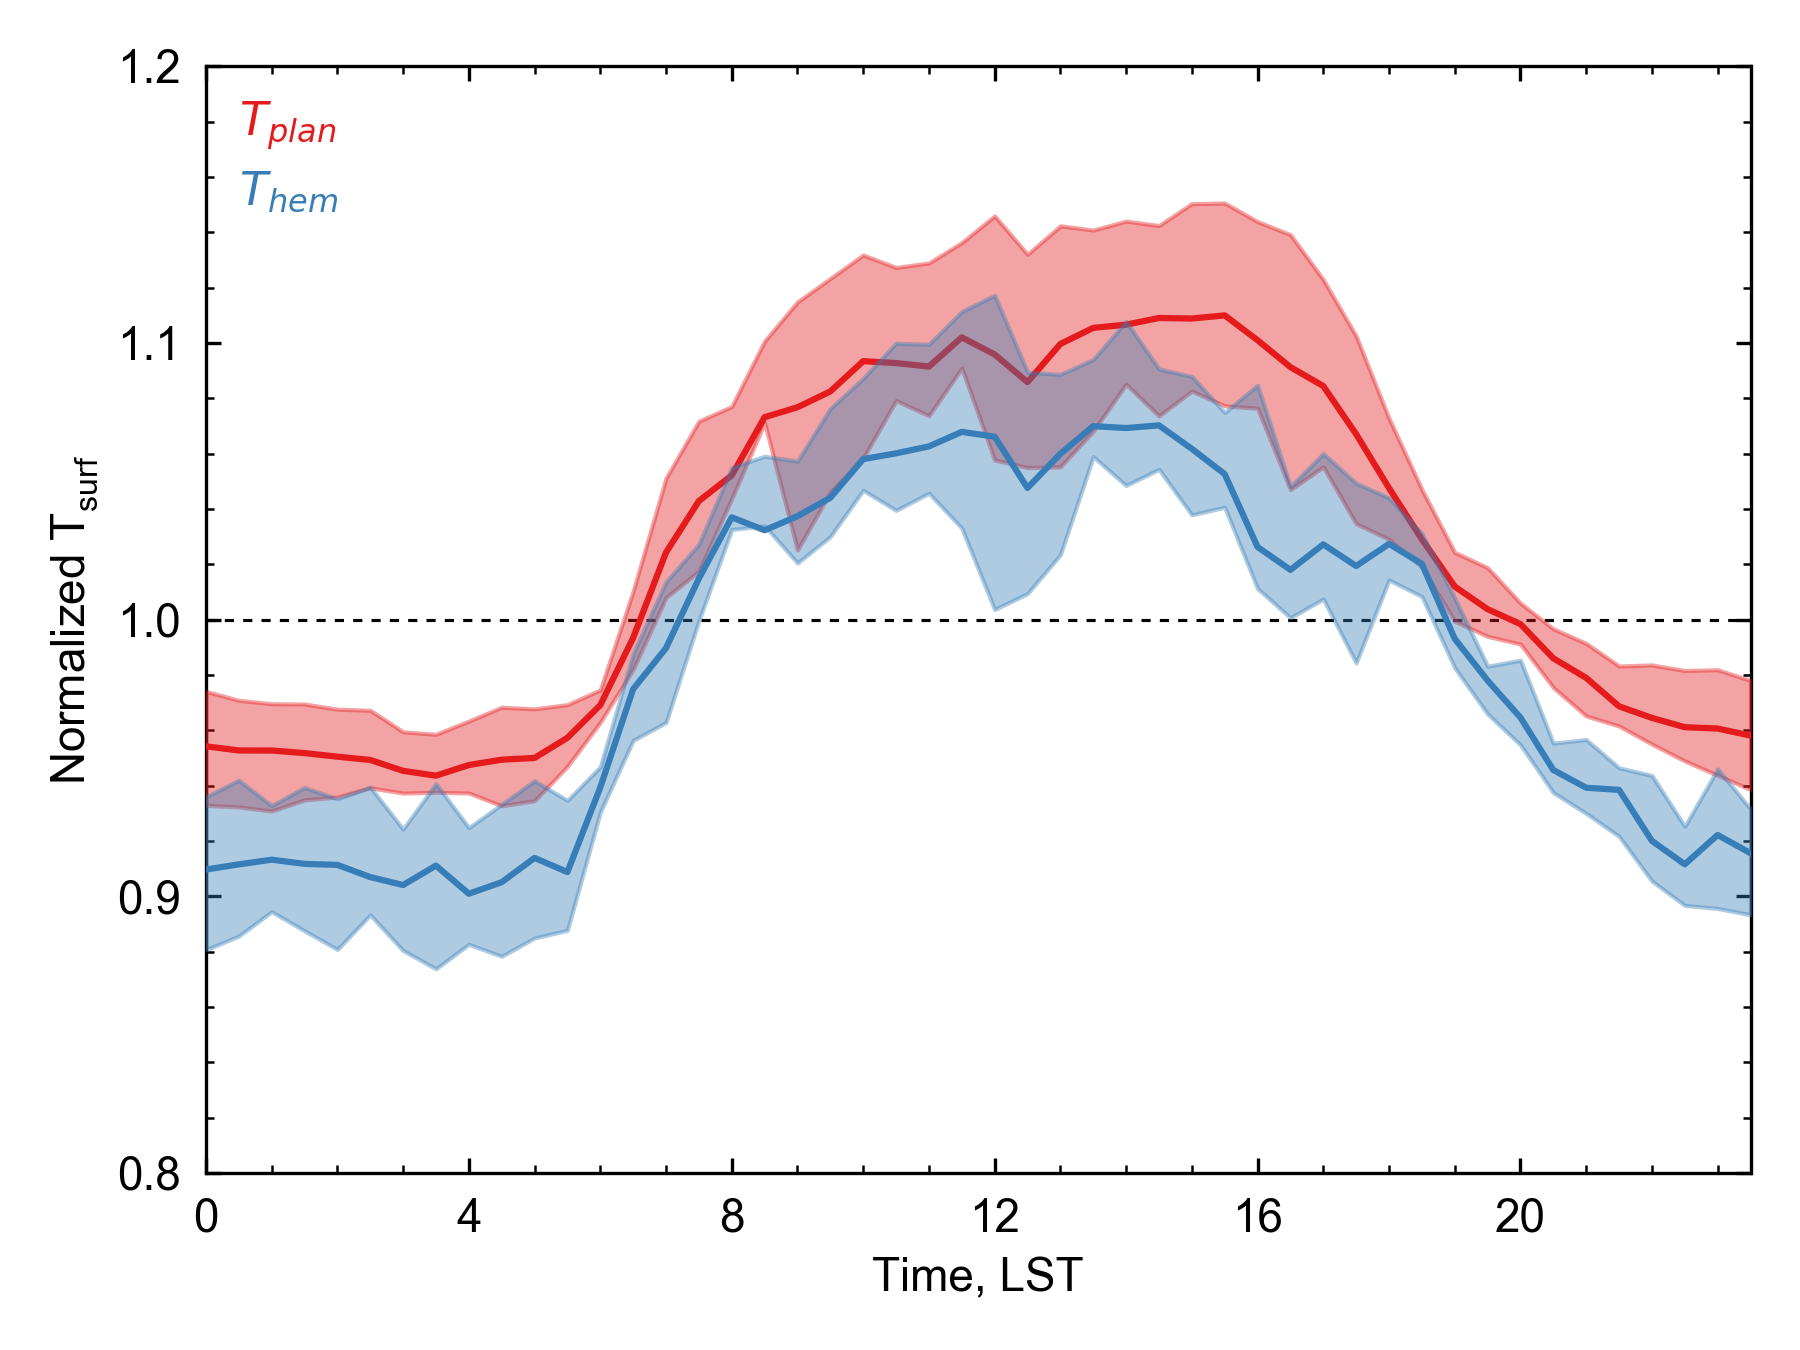
\includegraphics[width=15cm,
	height=7in,
	keepaspectratio]{nad_hem_314}
	\caption{A comparison of normalized T\textsubscript{hem, r} and T\textsubscript{plan} over the IOP. Shading indicates the area bounded by the first and third quartiles. n = 14}
	\label{tc_nadhem}
\end{figure}

\begin{figure}[H]
	\centering
	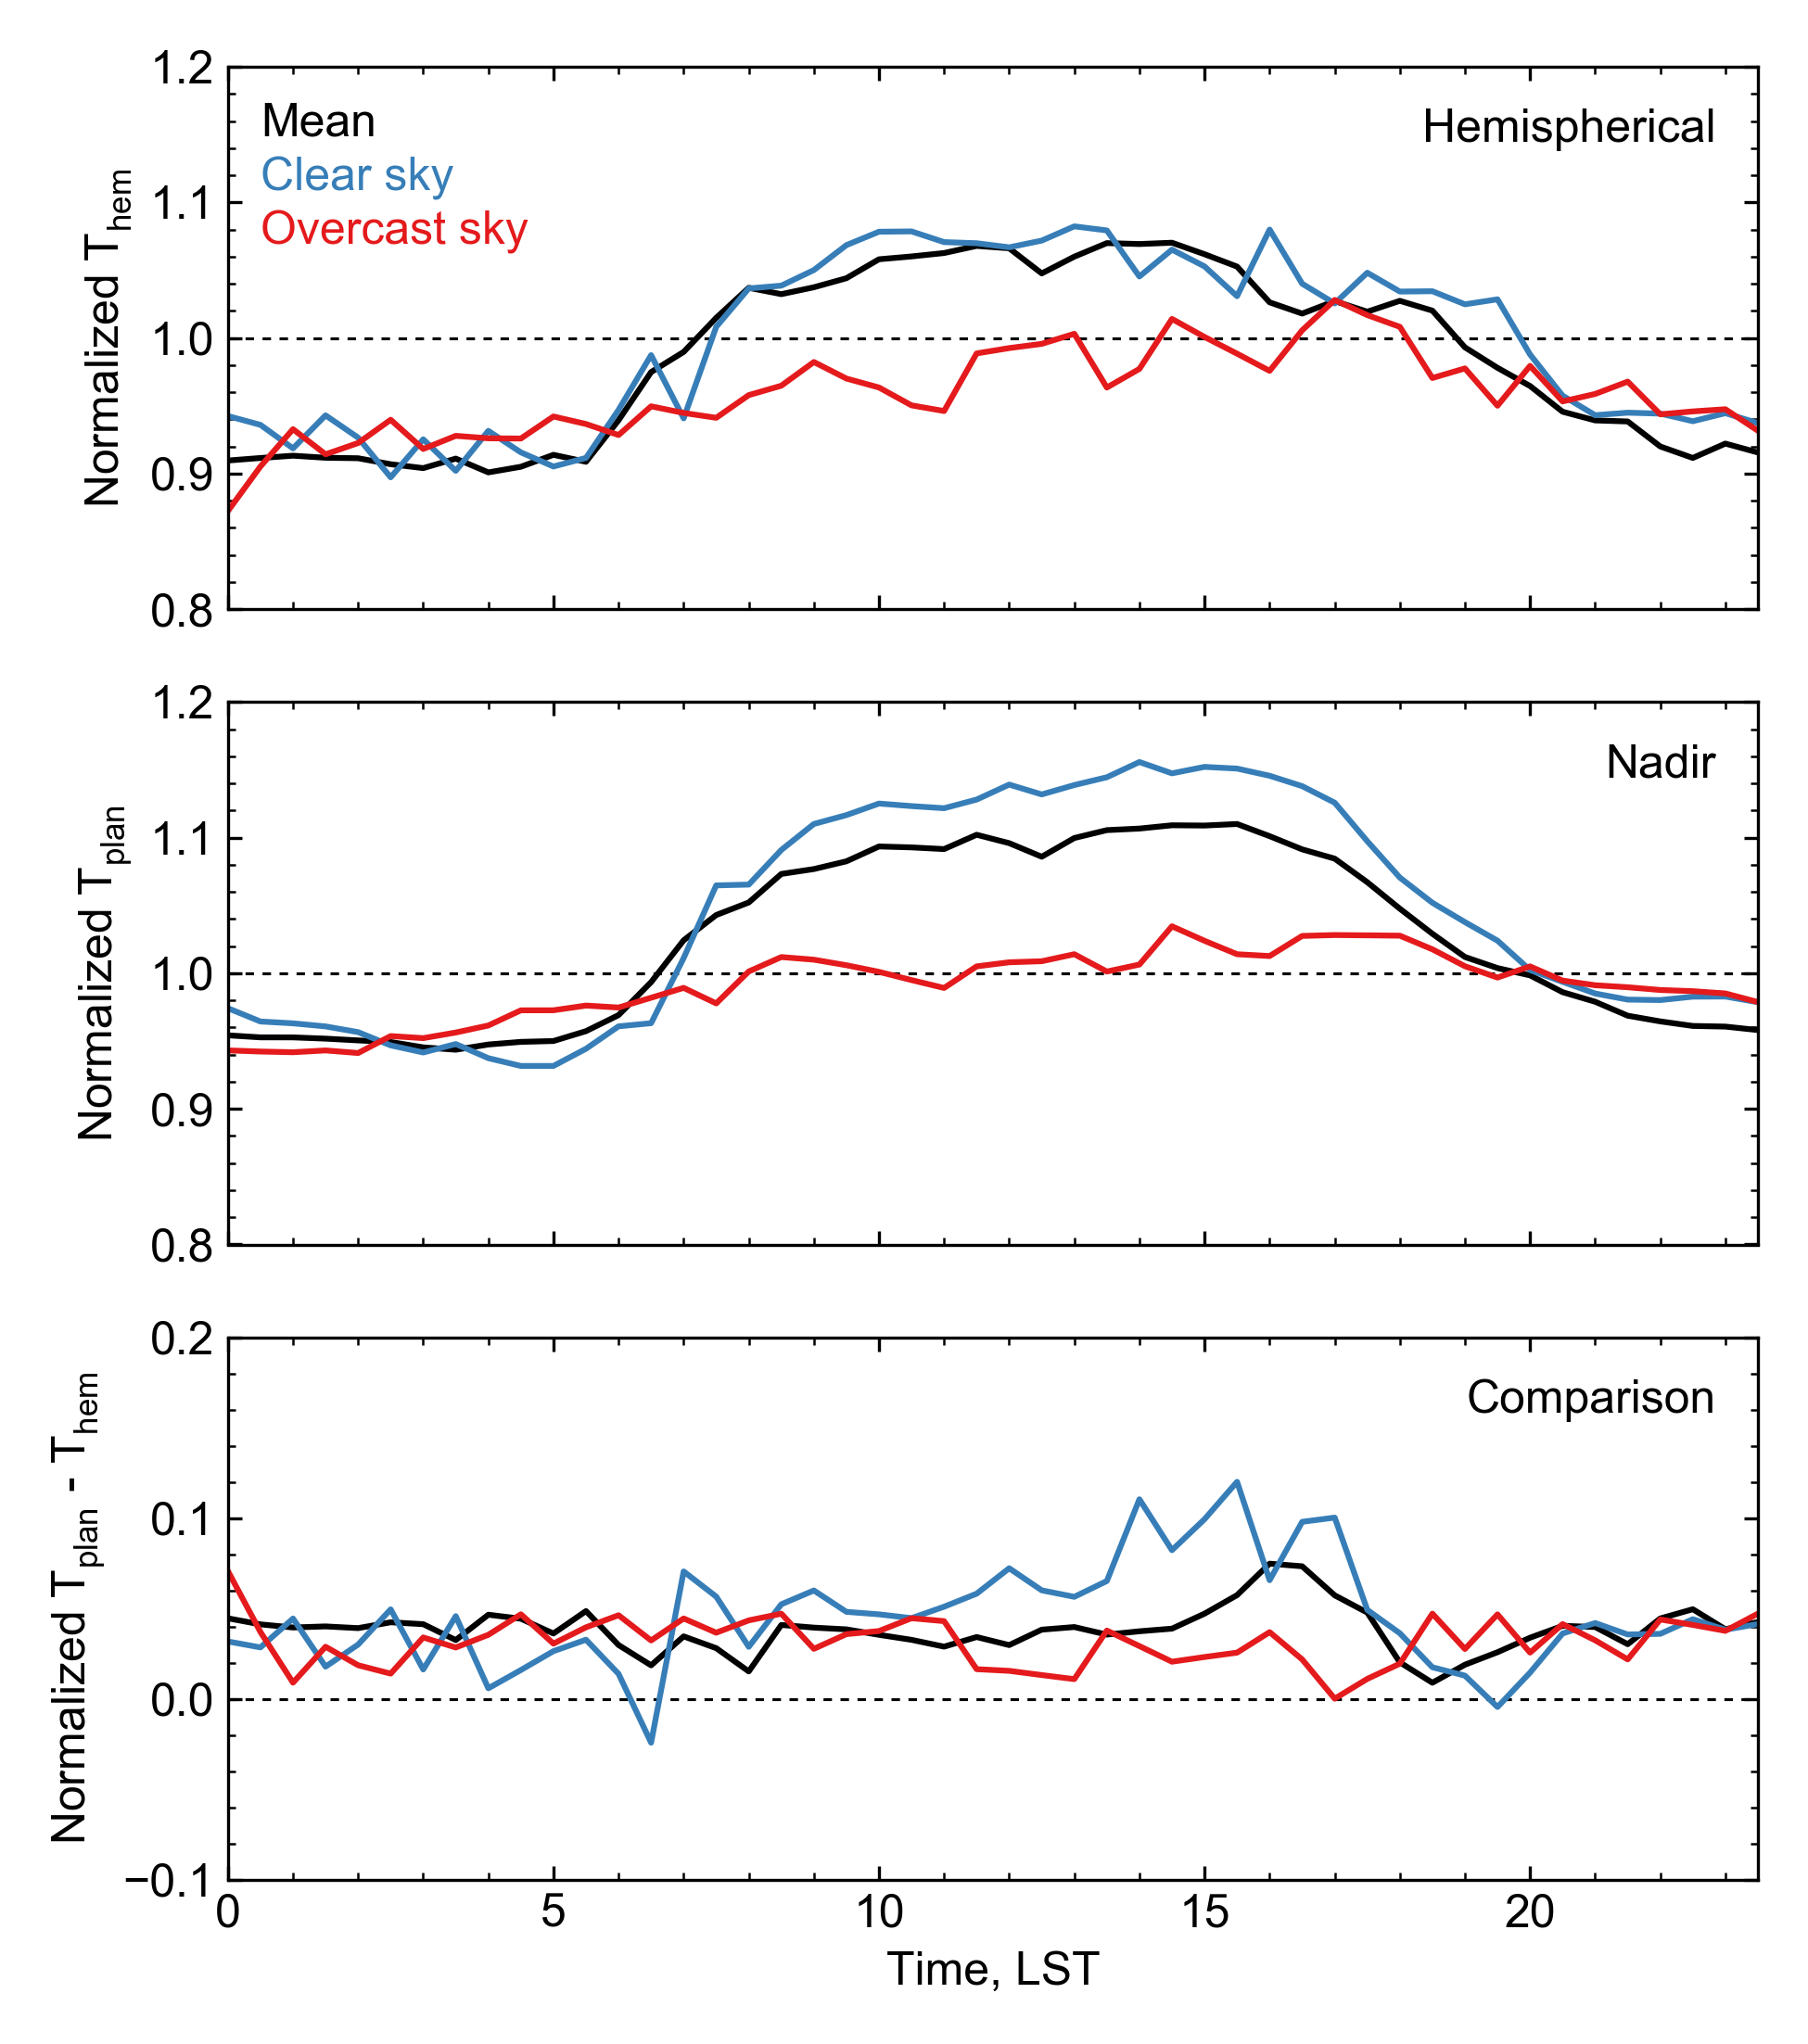
\includegraphics[width=15cm,
	height=7in,
	keepaspectratio]{tc_mean_314}
	\caption{Normalized T\textsubscript{hem, r}, T\textsubscript{plan}, and $\Delta$T\textsubscript{plan - hem, r} averaged over the IOP and for clear sky and overcast case days. n = 14}
	\label{tc_mean2}
\end{figure}

\section{Discussion}

\subsection{Controls on atmospheric correction magnitude}

Atmospheric correction magnitudes are highly dependent on factors that control $\Delta$T\textsubscript{surf - air}. With a non-zero $\Delta$T\textsubscript{surf - air}, TIR emitted from the surface and absorbed by the atmosphere is re-emitted at a different temperature, modifying the at-sensor TIR signal. Thus, the strength of the T\textsubscript{surf} to T\textsubscript{air} differential is directly related to the magnitude of atmospheric effects on a remote sensed TIR signal. This results in a strong positive relationship between atmospheric correction magnitude and $\Delta$T\textsubscript{hem, r - air}. Results show that conditions that maximize microscale surface to atmosphere thermal contrasts entail large correction magnitudes and conditions that suppress differences between T\textsubscript{surf} and T\textsubscript{air} show much smaller or negative correction magnitudes.

Of the meteorological variables tested, correction magnitudes are most strongly dependent on solar input. Solar radiation incident on the surface forces microscale thermal contrasts between the surface and the air, directly controlling the T\textsubscript{surf} - T\textsubscript{air} differential. The relationships between correction magnitude and T\textsubscript{hem, r} and T\textsubscript{air} individually are weaker and more complex. Correction magnitudes are smallest when T\textsubscript{hem, r} and T\textsubscript{air} are between approximately $10$ and $20$ \si{\degreeCelsius} - largely made up of morning and cloudy observations during the summer months where thermal contrasts between T\textsubscript{surf} and T\textsubscript{air} are small or weakly negative, forcing small correction magnitudes. During the winter months, a negative relationship between T\textsubscript{hem, r} and T\textsubscript{air} and correction magnitudes is observed, likely a result of the effect of shifting spectral emittance curves combined with non-uniform sensor response - discussed in section \ref{Persistence in correction magnitudes}. On clear sky summer days, positive relationships between correction magnitudes and T\textsubscript{hem, r} and T\textsubscript{air} are observed as an increased solar input foster higher overall temperatures and large contrasts between T\textsubscript{surf} and T\textsubscript{air}.

Results show significant seasonal, day to day, and diurnal variation in correction magnitudes. The range of observed correction magnitudes is largest in summer, when a wide range of mid latitude synoptic conditions result in significant contrasts in daytime solar input and consequently large variations in the T\textsubscript{surf} - T\textsubscript{air} differential. Maximum correction magnitudes over the study period (often approaching $7$ to $8$ \si{\kelvin}) occur frequently near solar noon on clear, hot, humid days, during which intense solar heating of the surface produces a large T\textsubscript{surf} - T\textsubscript{air} differential. Minimum correction magnitudes near $-1$ \si{\kelvin} occur consistently on clear, calm nights following hot days, when T\textsubscript{surf} can dip below T\textsubscript{air}, even in urban areas where canyon trapping of radiation reduces cooling rates for both T\textsubscript{surf} and T\textsubscript{air}. In winter, decreased variability in overall solar input results in less intense solar heating of the surface and smaller T\textsubscript{surf} - T\textsubscript{air} contrasts. Thus, winter correction magnitudes are smaller and more consistent with a mean of approximately $2$ \si{\kelvin}.

\subsection{The effect of non-uniform pyrgeometer spectral dome transmittance on correction magnitudes}\label{Persistence in correction magnitudes}

A pyrgeometer's dome transmittance is spectrally non-uniform. Thus, the "dome effect" a pyrgeometer exerts on a given incoming TIR signal changes as a function of emission temperature (T\textsubscript{emiss}) because the shape of a given spectral radiance curve (R\textsubscript{$\nu$}) is temperature dependent. This is illustrated in Figure \ref{nonuniform} by comparing the relative peaks and shape of a pyrgeometer dome transmittance curve for several R\textsubscript{$\nu$} (T\textsubscript{emiss}) for a range of typical urban T\textsubscript{emiss} (T\textsubscript{emiss} = 260 - 320 \si{\kelvin}, at 5 \si{\kelvin} increments). As each curve interacts with a different portion of the spectral dome transmittance curve (\textit{r\textsubscript{$\nu$}}), and \textit{r\textsubscript{$\nu$}} is spectrally non-uniform, the distinct spectral shapes of R\textsubscript{$\nu$} results in differential dome effects for each T\textsubscript{emiss}.

\begin{figure}[H]
	\centering
	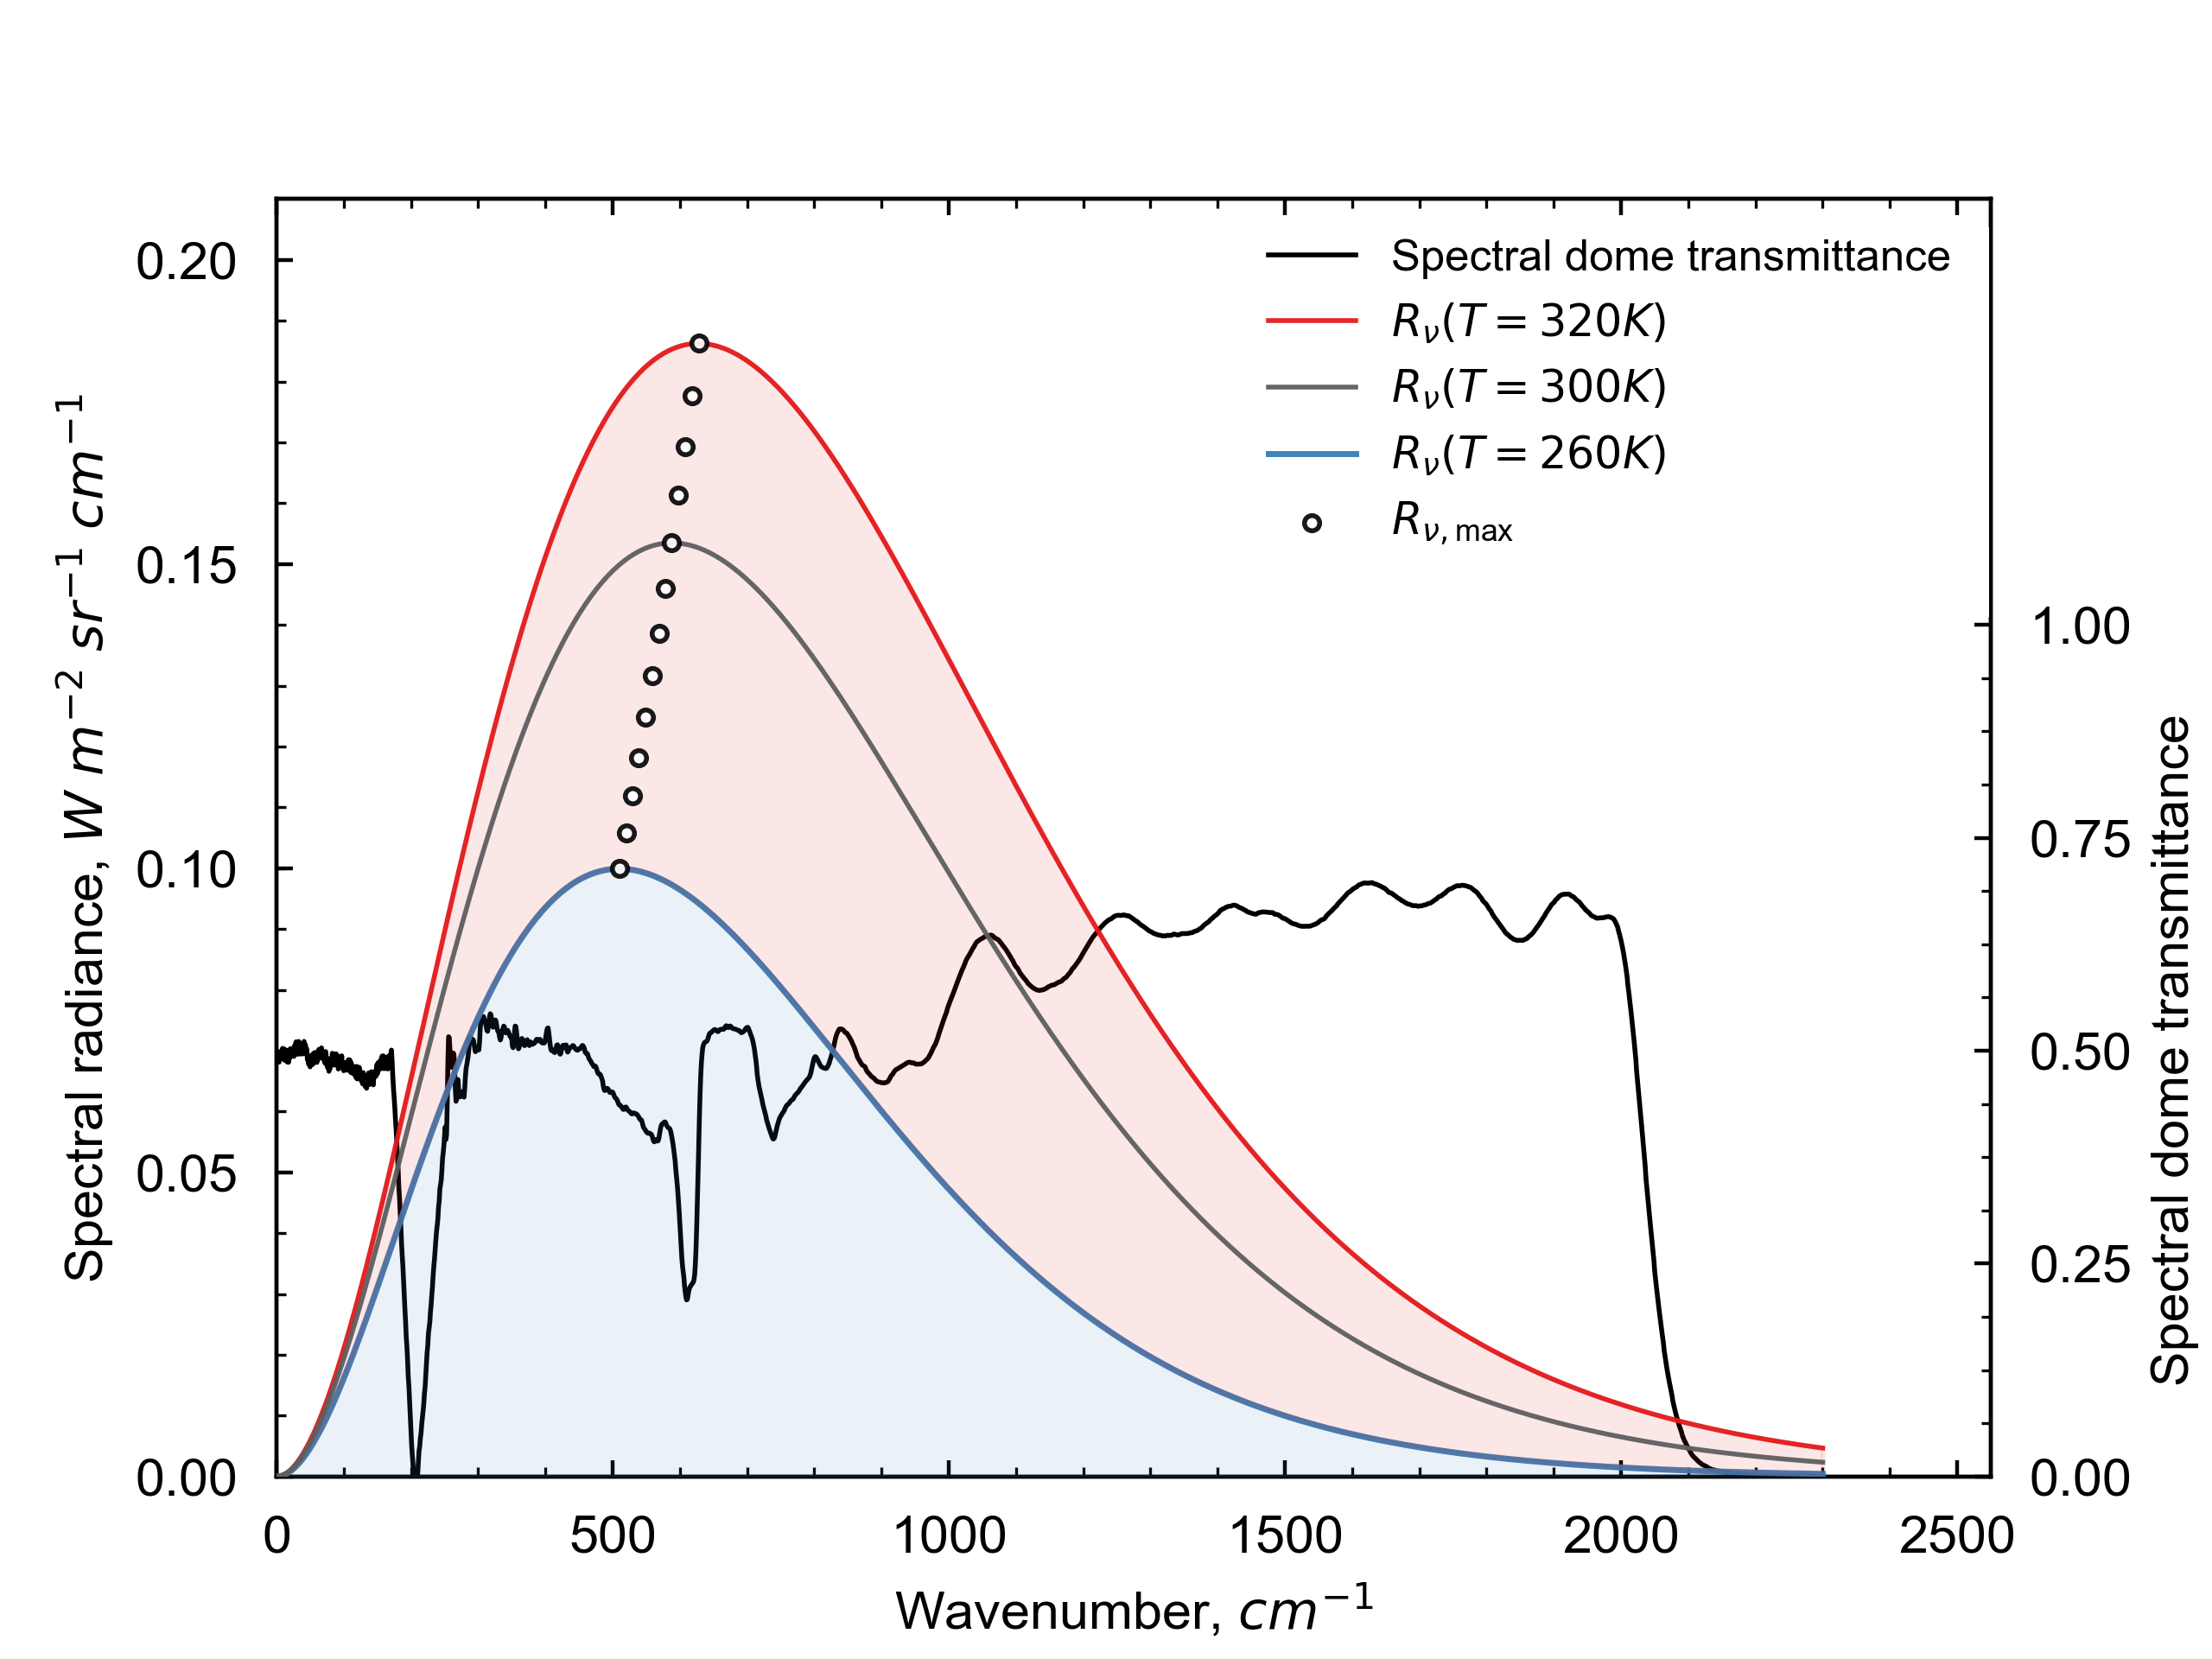
\includegraphics[width=15cm,
	height=7in,
	keepaspectratio]{nonuniform}
	\caption{Spectral dome transmittance for a Kipp \& Zonen pyrgeometer overlaid with a Planckian spectral radiance curve at T = 300 \si{\kelvin} and the same curve shifted to represent the shape and peak of a spectral radiance curve at T = 270 \si{\kelvin}.}
	\label{nonuniform}
\end{figure}

Spectrally non-uniform pyrgeometer dome transmittance results in differential dome effects on the R\textsubscript{$\nu$} for different T\textsubscript{emiss}. Thus, temperature specific calibration routines designed to remove dome effects and retrieve accurate irradiance values are subject to errors based on the difference between T\textsubscript{emiss} and the temperature at which the instrument was calibrated (T\textsubscript{calib}). The magnitude of this error can be expressed as differentials in Planck weighted mean sensor response ($\overline{r} $) calculated via equation \ref{meansens} for different T\textsubscript{emiss} --- where lower $\overline{r} $ indicates a larger dome effect on the signal received by the sensor. In addition, this error can be expressed as a dome adjusted temperature bias (T\textsubscript{bias}) computed as the difference between a reference T\textsubscript{calib} and a dome adjusted temperature (T\textsubscript{adj}). With R\textsubscript{$\nu$} (T\textsubscript{adj}) representing a spectral curve with the same integrated radiance as R\textsubscript{$\nu$} (T\textsubscript{calib}) shifted to represent the dome effect incurred at the target T\textsubscript{emiss}. For example, to calculate T\textsubscript{bias} for T\textsubscript{emiss} = 270 \si{\kelvin} at T\textsubscript{calib} = 300 \si{\kelvin}, a spectral shift is applied to R\textsubscript{$\nu$} (300 \si{\kelvin}) so that its peak spectral radiance matches the wavenumber of peak spectral emission for R\textsubscript{$\nu$} (270 \si{\kelvin}). When integrated, the two curves have the same radiance, but interact with \textit{r} over different wavebands. Following the spectral shift, spectral radiances are convolved by the dome transmittance function, integrated over the waveband and hemisphere, and used to derive T\textsubscript{adj} via equation \ref{stefb1} with $\overline{r}$ at T\textsubscript{calib}.\footnote{In this sensitivity test, the waveband was truncated from 1 - 2500 \si{cm^{-1}} to 80 - 2500 \si{cm^{-1}} to accommodate shorter wavenumber when shifting R\textsubscript{$\nu$} (T\textsubscript{calib}) to lower temperatures where peak spectral emission occurs at smaller wavenumber. This results in a slight underestimation of the total radiance at a given T\textsubscript{emiss}, and thus, slightly negative T\textsubscript{bias} at T\textsubscript{calib}, where no spectral shift has been applied. When computed from total in band radiance, T\textsubscript{bias} at the reference T\textsubscript{calib} is zero.} Table \ref{nonuniformsen} shows $\overline{r}$ and T\textsubscript{bias} and for a range of T\textsubscript{emiss}.

\begin{table}[H]
	\centering
	\caption{Planck weighted mean sensor response and T\textsubscript{bias} for a suite of common urban emission temperatures.}
	\label{nonuniformsen}
	\begin{tabular}{p{1.5cm}p{1.5cm}c}
		\toprule 
		& & T\textsubscript{bias}, \si{\kelvin} \\
		T\textsubscript{emiss}, \si{\kelvin}& $\overline{r}$, \% & computed for T\textsubscript{calib} = 300 \si{\kelvin} \\ \midrule
		%Emission temperature, \si{\kelvin}& $\overline{r}$, \% & T\textsubscript{adj}, \si{\kelvin} \\ \midrule
		260 & 48.3 & -1.67 \\ 
		265 & 48.5 & -1.49 \\ 
		270 & 48.7 & -1.32 \\ 
		275 & 48.9 & -1.13 \\ 
		280 & 49.1 & -0.95 \\ 
		285 & 49.3 & -0.75 \\ 
		290 & 49.4 & -0.56 \\ 
		295 & 49.6 & -0.36 \\ 
		300 & 49.7 & -0.15 \\ 
		305 & 50.0 & 0.05 \\ 
		310 & 50.1 & 0.26  \\ 
		315 & 50.3 & 0.47 \\ 
		320 & 50.4 & 0.69  \\
		\bottomrule
	\end{tabular} 
\end{table}

The magnitude of T\textsubscript{bias} increases as the difference between the reference T\textsubscript{calib} and T\textsubscript{emiss} increases, with approximately equal rates of change with increasing and decreasing T\textsubscript{emiss}. Dome effects have a significant effect on the pyrgeometer received signal when comparing irradiances or T\textsubscript{hem} over a wide range of temperatures, or when T\textsubscript{emiss} is significantly different from T\textsubscript{calib}. Pyrgeometers used in the BUBBLE campaign were calibrated outdoors under clear-sky, mid-latitude springtime conditions \citep{Christen2005}. Thus, dome effects inherent in uncorrected $L_z$ measurements in this study are likely smaller in summer than in winter (as T\textsubscript{emiss} is likely closer to T\textsubscript{calib} in summer than it is in winter), and are well represented by Table \ref{nonuniformsen}.

By convolving modeled spectral radiances by a dome transmittance curve, the correction method presented in this study accounts for dome effects. Thus, correction magnitudes include both atmospheric effects and effects from spectrally non-uniform dome transmittance (and, crudely, emissivity effects, as modeled radiances are calculated with $\epsilon$ = 0.95 and include a reflected L\textsubscript{sky} component). While the individual effects are difficult to separate, temperature dependent differential dome effects are visible in correction magnitudes as a persistent minor positive correction in winter. Relative to T\textsubscript{calib}, lower T\textsubscript{emiss} in winter results in a larger dome effects. This manifests in artificially low T\textsubscript{hem, b} and increased wintertime correction magnitudes. 

Additionally, modeled irradiances include a reflected downwelling component, which, although small, is sensitive to T\textsubscript{air} and humidity profiles above the sensor height. Because these data were not consistently measured, mid-latitude summer and winter standard atmospheric profiles supplemented the measured data. The climate of Basel is characterized by mild, humid winters (K\"oppen classification: Cfb). As a result, above-sensor T\textsubscript{air} and humidity values are likely underestimated by the standard wintertime atmosphere, reducing the modeled at-sensor reflected component of downwelling longwave in winter and the overall modeled at-sensor signal. This results in an increase in derived T\textsubscript{hem, r} and correction magnitudes as measured irradiances are matched with irradiances modeled at slightly higher T\textsubscript{surf} to make up for the underestimated at-sensor L\textsubscript{sky} signal. 

%Differential dome effects are visible in atmospheric corrections as a persistent minor positive correction in winter. During winter T\textsubscript{arg} This has the effect of positively weighting spectral bands with less energy and negatively weighting bands with more energy, resulting in a small systemic underestimation of the broadband signal which is removed during instrument calibration. However, calibration routines are specific to a range of T\textsubscript{surf} and the effect of the sensor's non-uniform spectral response changes based on emitter temperature. Lower emitter temperatures shift the peak of the Planckian curve closer to bands with low relative sensor response. Thus, T\textsubscript{bright} inverted from pyrgeometer measured irradiance via \ref{stefb1} is systemically lower than those derived using a routine that accounts for nonuniform sensor response. In other words, because a pyrgeometer does not respond uniformly over a spectral longwave curve and operates over a slightly restricted longwave bandpass, T\textsubscript{bright} will always include some small underestimation of T\textsubscript{rad}, even when atmospheric influence is negligible. The size of this underestimation is inversely related to T\textsubscript{surf} - increasing the base magnitude of wintertime corrections compared to summertime corrections. Additionally, modeled irradiances include a reflected downwelling component, which, although small, is sensitive to T\textsubscript{air} and humidity profiles above the sensor height. Because this data was not consistently measured, mid-latitude summer and winter standard atmospheric profiles were supplemented. Basel's climate is characterized by mild, humid winters (K\"oppen classification: Cfb). As a result, above-sensor profiles of T\textsubscript{air} and humidity at study site are likely underestimated by the standard wintertime atmosphere, reducing the modeled at-sensor reflected component of downwelling longwave in winter. This results in an increase in both derived T\textsubscript{hem, r} and correction magnitudes. 

\subsection{The effect of sensor sampling geometry on remote sensed T\textsubscript{surf}}

Results show that sensor sampling regimes have a significant effect on remotely sensed T\textsubscript{surf}. Both T\textsubscript{hem, r} and T\textsubscript{plan} overestimate T\textsubscript{comp} by day and underestimate T\textsubscript{comp} by night. However, over/underestimations from geometric effects are highly dependent on synoptic conditions, particularly for a nadir view of the urban surface. T\textsubscript{plan} is much greater than T\textsubscript{comp} under clear sky conditions, with T\textsubscript{hem, r} showing a much smaller positive bias. Over half of the T\textsubscript{plan} signal from the Sperrstrasse canyon is generated by rooftops that have both a large diurnal T\textsubscript{surf} amplitude and the highest daytime facet T\textsubscript{max}. Undersampling of sloped facets and neglect of wall facets by T\textsubscript{plan} also has a significant effect on the daytime clear-sky warming bias, as walls show much cooler daytime T\textsubscript{max} than T\textsubscript{roof} or T\textsubscript{road} and have a moderating effect on T\textsubscript{comp} and T\textsubscript{hem, r} by day, particularly on hot clear sky days. Mean daytime overestimations by T\textsubscript{plan} just after solar noon are approximately $4$ \si{K} over the IOP, approaching $8$ \si{K} on the clear sky case day. T\textsubscript{hem, r} shows smaller overestimations of approximately $3$ \si{K} over the IOP and $5$ \si{K} on the clear sky case day. Urban T\textsubscript{surf} and the sUHI are often measured from satellite TIR remote sensors that retrieve T\textsubscript{plan} exclusively under clear-sky conditions and often sample in the nadir. Thus, overestimation of daytime urban T\textsubscript{comp} inherent in the satellite T\textsubscript{surf} record is best represented by T\textsubscript{plan} on the clear sky case day. 

Nighttime underestimations of T\textsubscript{comp} by nadir and hemispherical views are a result of an undersampling of wall and road facets respectively. T\textsubscript{hem, r} derived from $L_z$ measured at the Sperrstrasse canyon oversamples the nearest roof and underestimates the canyon floor compared to T\textsubscript{comp} as its location along the canyon axis is skewed towards the south facing wall (rather than the center of the canyon) and its height is approximately 2.17 times mean building height. Non-optimal sensor placement in the Sperrstrasse canyon results in a large underestimation of nighttime T\textsubscript{comp} by T\textsubscript{hem, r}. However, nighttime underestimation --- and to some extent, daytime overestimation --- by T\textsubscript{hem, r} is the combined result of a sampling bias inherent in a hemispherical view of the surface and improper sensor placement, discussed in greater detail in section \ref{Methodological limitations and considerations}. Thus, both of these biases can likely be reduced significantly by adjusting sensor placement to best represent surface geometry. 

\section{Sensor placement sensitivity testing} \label{Methodological limitations and considerations}

 When measured from a near ground downward facing pyrgeometer, upwelling TIR is sensitive to sensor height and position relative to surface geometry \citep{Adderley2015, Roberts2010}. Below 3 times mean roof level, measured TIR varies from a "true", geometrically representative, TIR signal based on a comparison between facet view factor proportions of the sensor and those of the urban surface. A perfectly geometrically representative remote sensed TIR signal is one measured from a sensor with facet view factor proportions equaling those of the urban surface. I.e. for an urban surface made up of 50\% wall, 25\% road, and 25\% roof, a perfectly geometrically representative remote sensed signal would be one "seen" by a sensor with the same fractional facet view factor proportions. For an idealized, orthogonal, block-like urban array, \citet{Roberts2010} found that facet view factor proportions --- and thus measured TIR --- varied significantly with sensor position and height. To investigate the effect of sensor placement on T\textsubscript{hem, r} for a simplified representation of the Sperrstrasse canyon site, we used SUM to vary sensor position over a simplified DBM and calculate normalized view factor proportions for a 160\si{\degree} FOV sensor. For nine sensor positions, show in Figure \ref{placement}, facet view factor proportions normalized to unity are shown in Figure \ref{bars1} for a sensor height of 2.17 times mean building height and in Figure \ref{bars45} for a sensor height of 3 times mean building height. Approximated actual facet surface area proportions for the Sperrstrasse canyon are included for reference. A fully geometrically representative sensor viewing the urban surface would have facet view factor proportions equal to actual facet surface area proportions. 
  
 Normalized facet view factors show significant variation based on sensor position at both test heights. At the lower test height, varying sensor position perpendicular to the canyon axis, positions at the canyon center (positions 4, 5, and 6) are most representative of actual facet view factors, with decreasing representivity at the edge of the canyon (positions 1, 2, and 3), and over the rooftops (positions 7, 8, and 9). Moving the sensor parallel to the canyon axis, positions slightly offset from the roof edge (positions 2, 5, and 8) agree most closely with actual canyon surface area proportions, with decreasing representivity in positions further from the roof edge. Roof and road view factor proportions are most strongly affected by sensor placement. Positions directly over buildings show large biases towards roof view factors and positions in the center of the canyon showing slight biases towards road facets. In all positions roof view factor was overestimated (save position 4), and wall view factor was underestimated.
 
 \begin{figure}[H]
	\centering
	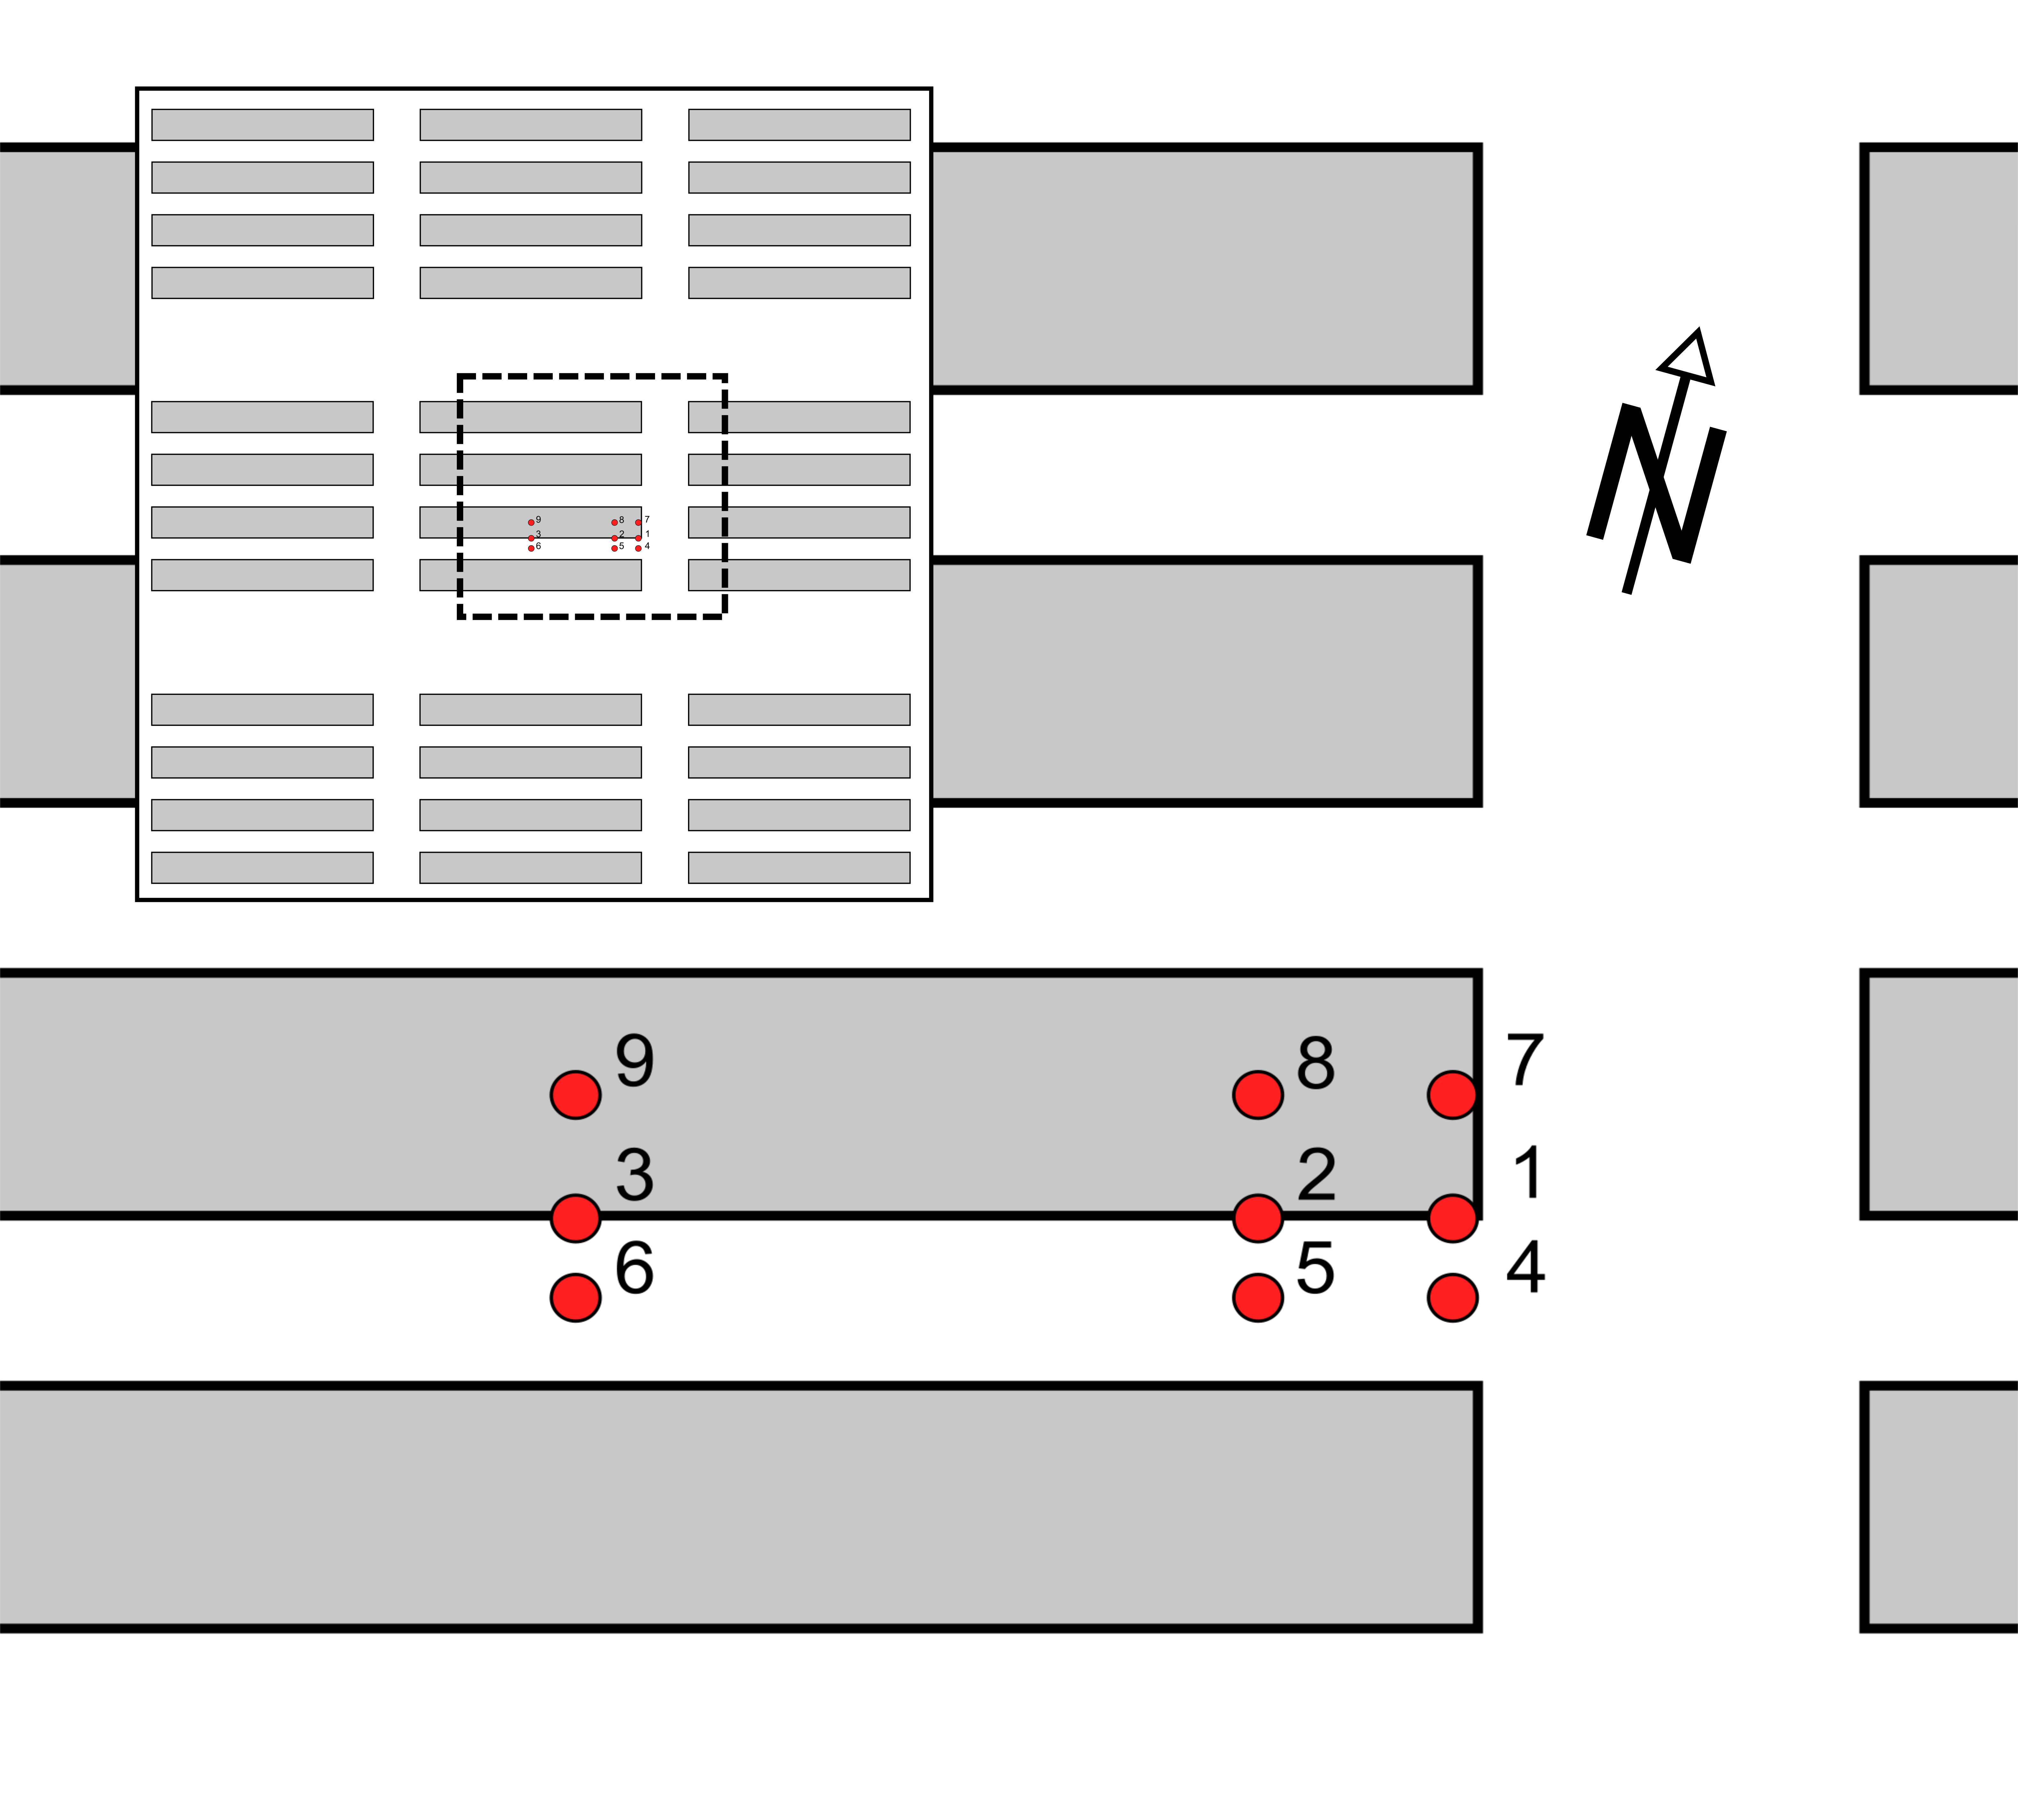
\includegraphics[width=15cm,
	height=7in,
	keepaspectratio]{placement2}
	\caption{A plan view of the simplified DBM showing the nine test sensor placements. Actual sensor placement at the Sperrstrasse canyon is approximated by number 3.}
	\label{placement}
\end{figure}

 \begin{figure}[H]
	\centering
	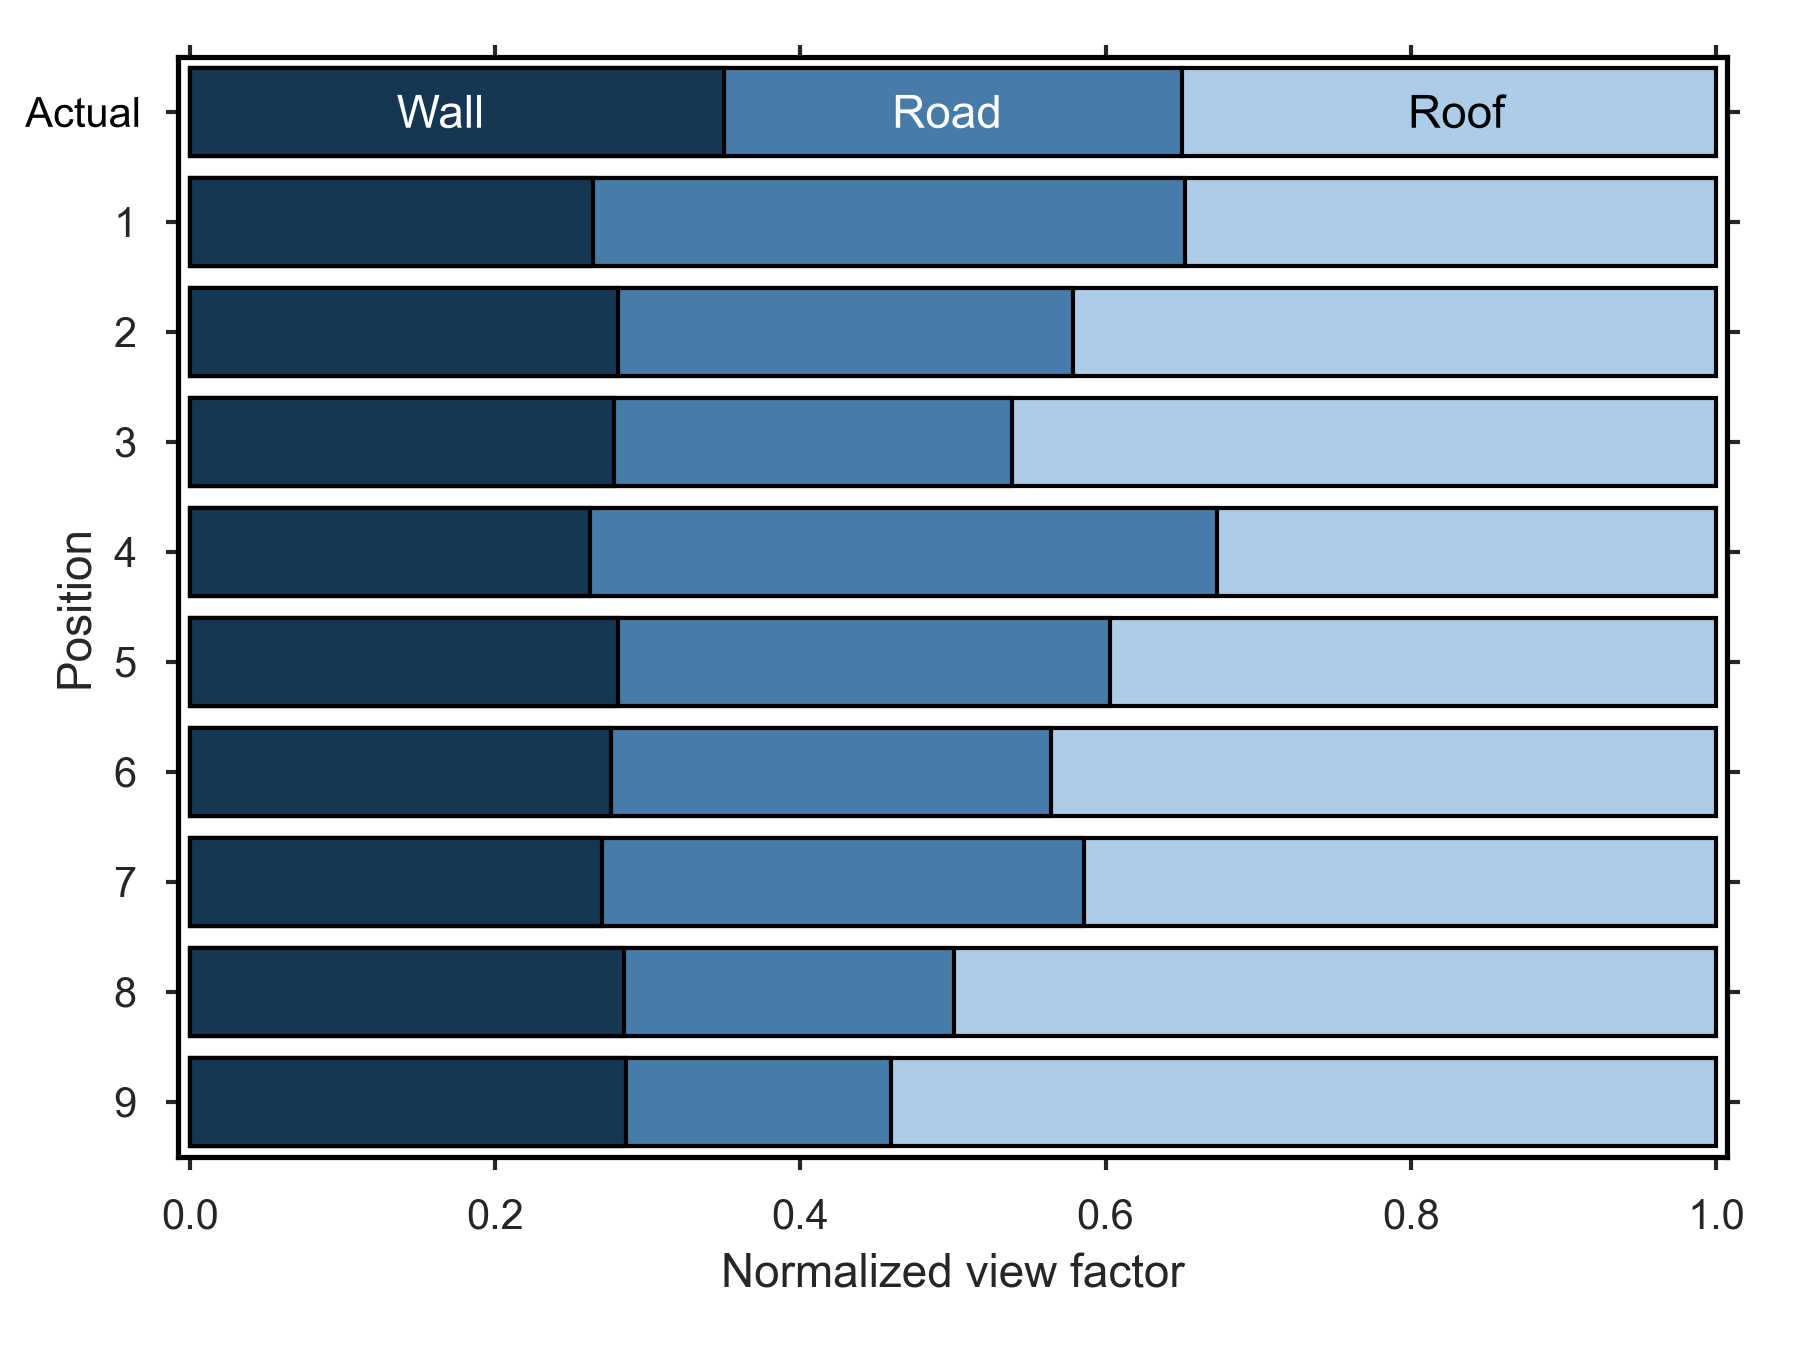
\includegraphics[width=15cm,
	height=7in,
	keepaspectratio]{bars2_ann}
	\caption{Normalized wall, road, and roof view factors for nine sensor positions viewing the simplified street canyon array from 2.17 times mean building height. Actual normalized view factors refer to surface area proportions for the three facet types in the Sperrstrasse street canyon. }
	\label{bars1}
 \end{figure}

Results in \citet{Adderley2015} and \citet{Roberts2010} show that sensitivity to sensor placement decreases as sensor height increases. Depending on surface geometry, sensor view factor proportions and the TIR signal "seen" by a sensor become spatially invariant sensor at heights above approximately 3 to 5 times mean building height. Results from the higher sensor test height support findings in \citet{Adderley2015} and \citet{Roberts2010}, with decreased spatial variance in facet view factor proportions across the nine sensor positions. However increased spatial stability in view factor proportions does not necessarily entail increased geometric representivity. For all sensor placements, road view factor proportion is increased and wall view factor is reduced. This results in large overestimations of road view factor for nearly all positions except positions 3 and 9, which include a large overestimation of roof view factor. Thus, although increasing sensor height does increase spatial invariance, it can lead to decreased representivity for some positions - in this case, positions 1 and 4.

\begin{figure}[H]
	\centering
	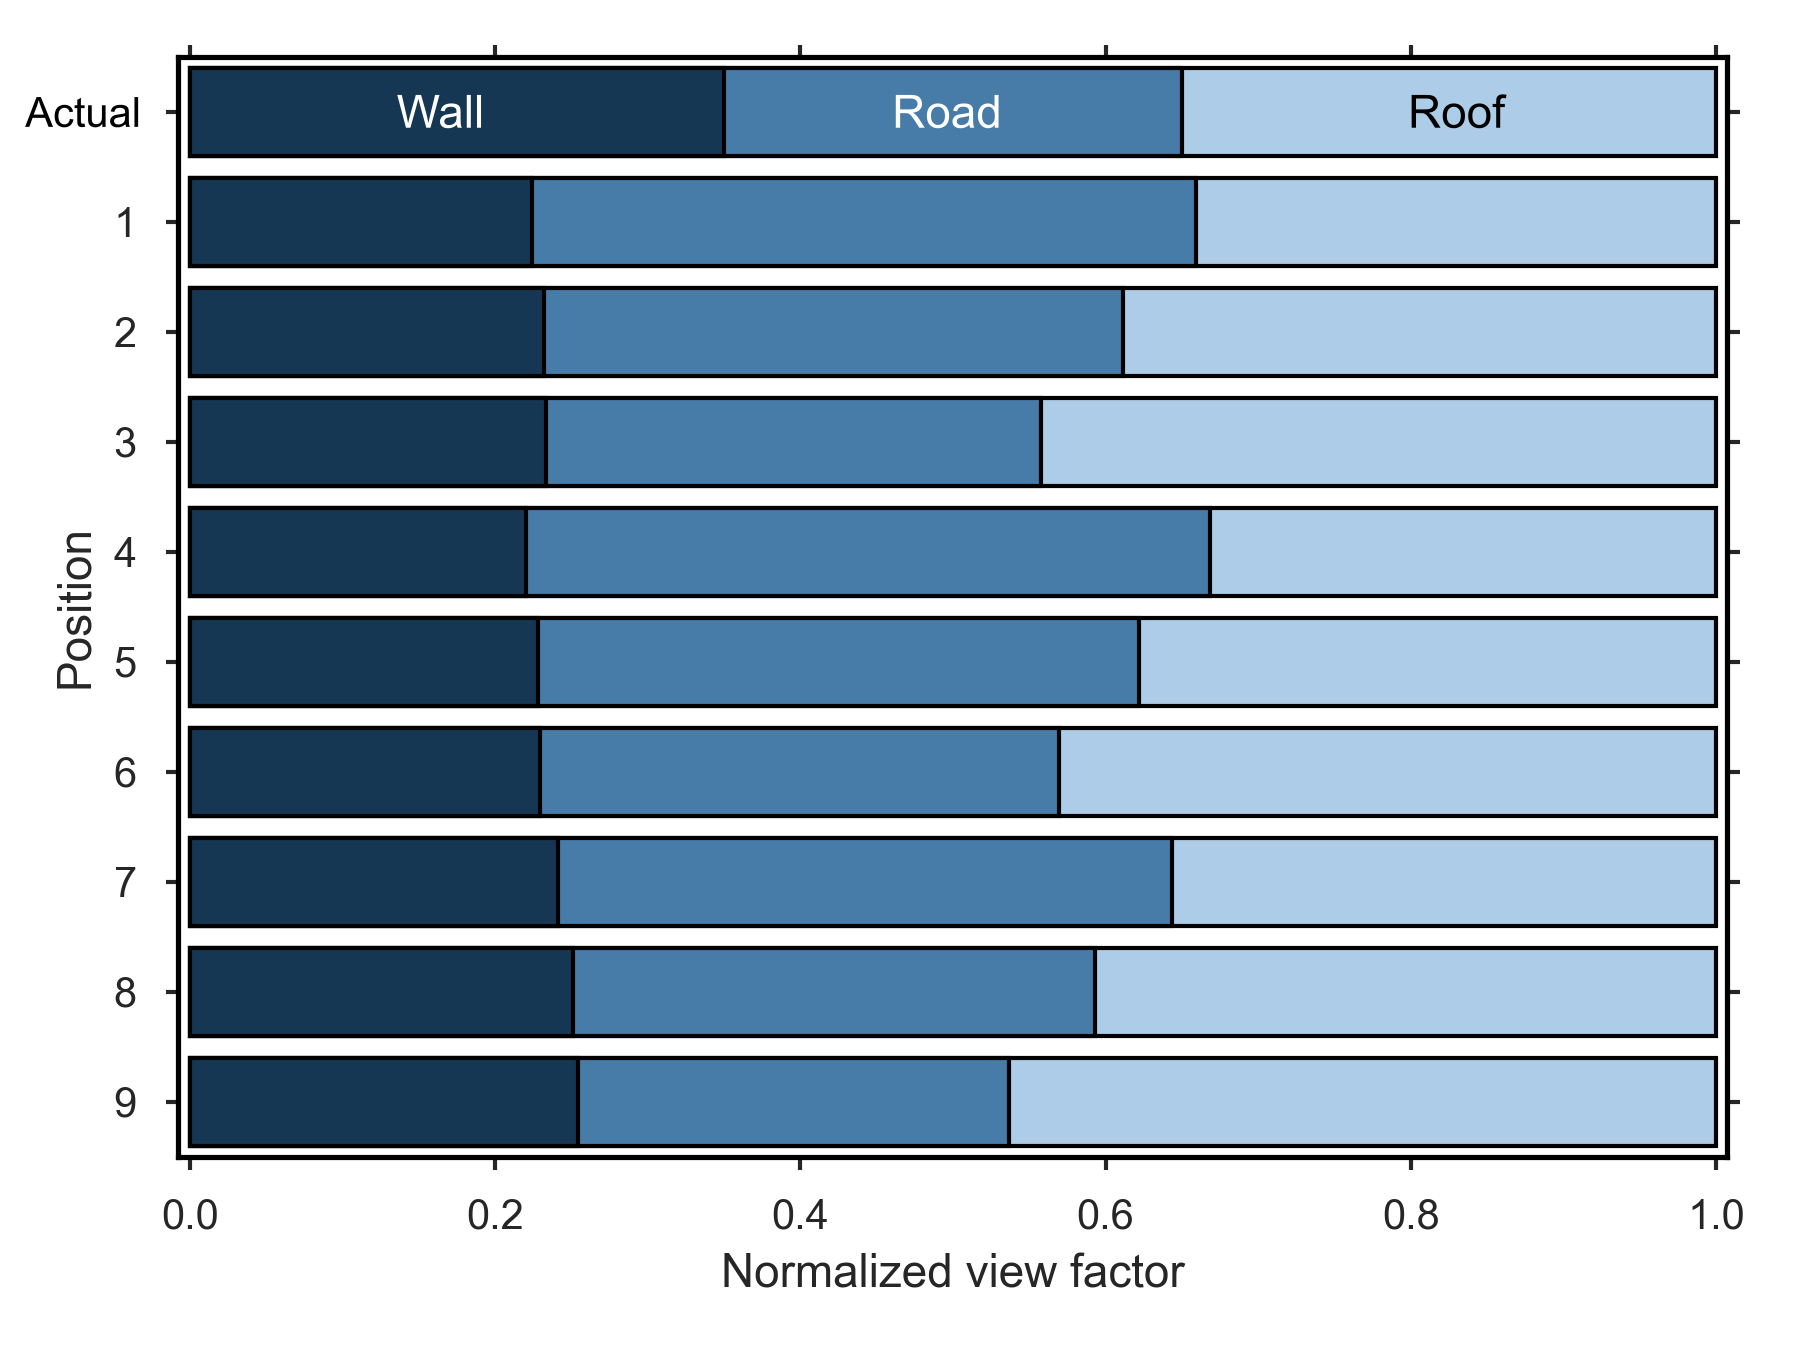
\includegraphics[width=15cm,
	height=7in,
	keepaspectratio]{bars45_ann}
	\caption{Normalized wall, road, and roof view factors for nine sensor positions viewing the simplified street canyon array from 3 times mean building height. Actual normalized view factors refer to surface area proportions for the three facet types in the Sperrstrasse street canyon. }
	\label{bars45}
\end{figure}

To visualize how sensor placement affects T\textsubscript{hem, r} retrieved via the method detailed in this study, T\textsubscript{hem, r} is inferred using wall, roof, and road view factors calculated in SUM for the two sensor heights to compute a weighted average of T\textsubscript{wall}, T\textsubscript{road}, and T\textsubscript{roof} for each sensor position at 30 minute intervals over the IOP. Temperatures are normalized by T\textsubscript{comp} and averaged at each time step over the IOP, the results of which are shown in Figures \ref{vf_all} and \ref{vf_all45}. As is the case with view factor proportions, T\textsubscript{hem, r} is highly dependent on sensor placement. For the lower sensor height, as predicted by view factor proportions, positions at the center of the canyon (positions 4, 5, and 6) and edge of the building (positions 1, 4, and 7) follow T\textsubscript{comp} most closely. By day, all sensor positions overestimate T\textsubscript{comp}, from a systemic bias towards rooftop facets. The degree of overestimation is largely determined by rooftop view factor, with larger overestimations coming from positions most biased towards hot rooftop surfaces. At night, most sensor positions (save position 4) underestimate T\textsubscript{comp}, again from a bias towards cool rooftop facets. Position 4 weakly overestimates nighttime T\textsubscript{comp}, from a slight view factor bias towards road facets with suppressed nocturnal cooling from canyon radiation trapping. 

At the higher test height, T\textsubscript{hem, r} is more representative of T\textsubscript{comp} for positions 2, 3, and 5 - 9. T\textsubscript{hem, r} from positions 1 and 4 display a slight systematic overestimation of T\textsubscript{comp}. For these positions, although roof view factor proportion is well represented, road view factor is significantly overestimated, oversampling warmer nighttime road temperatures. For all other positions, daytime overestimation and nighttime underestimation of T\textsubscript{comp} is reduced. Thus, as is the case with view factor proportions, at the higher test height, T\textsubscript{hem, r} is more spatially stable.
 
   \begin{figure}[H]
 	\centering
 	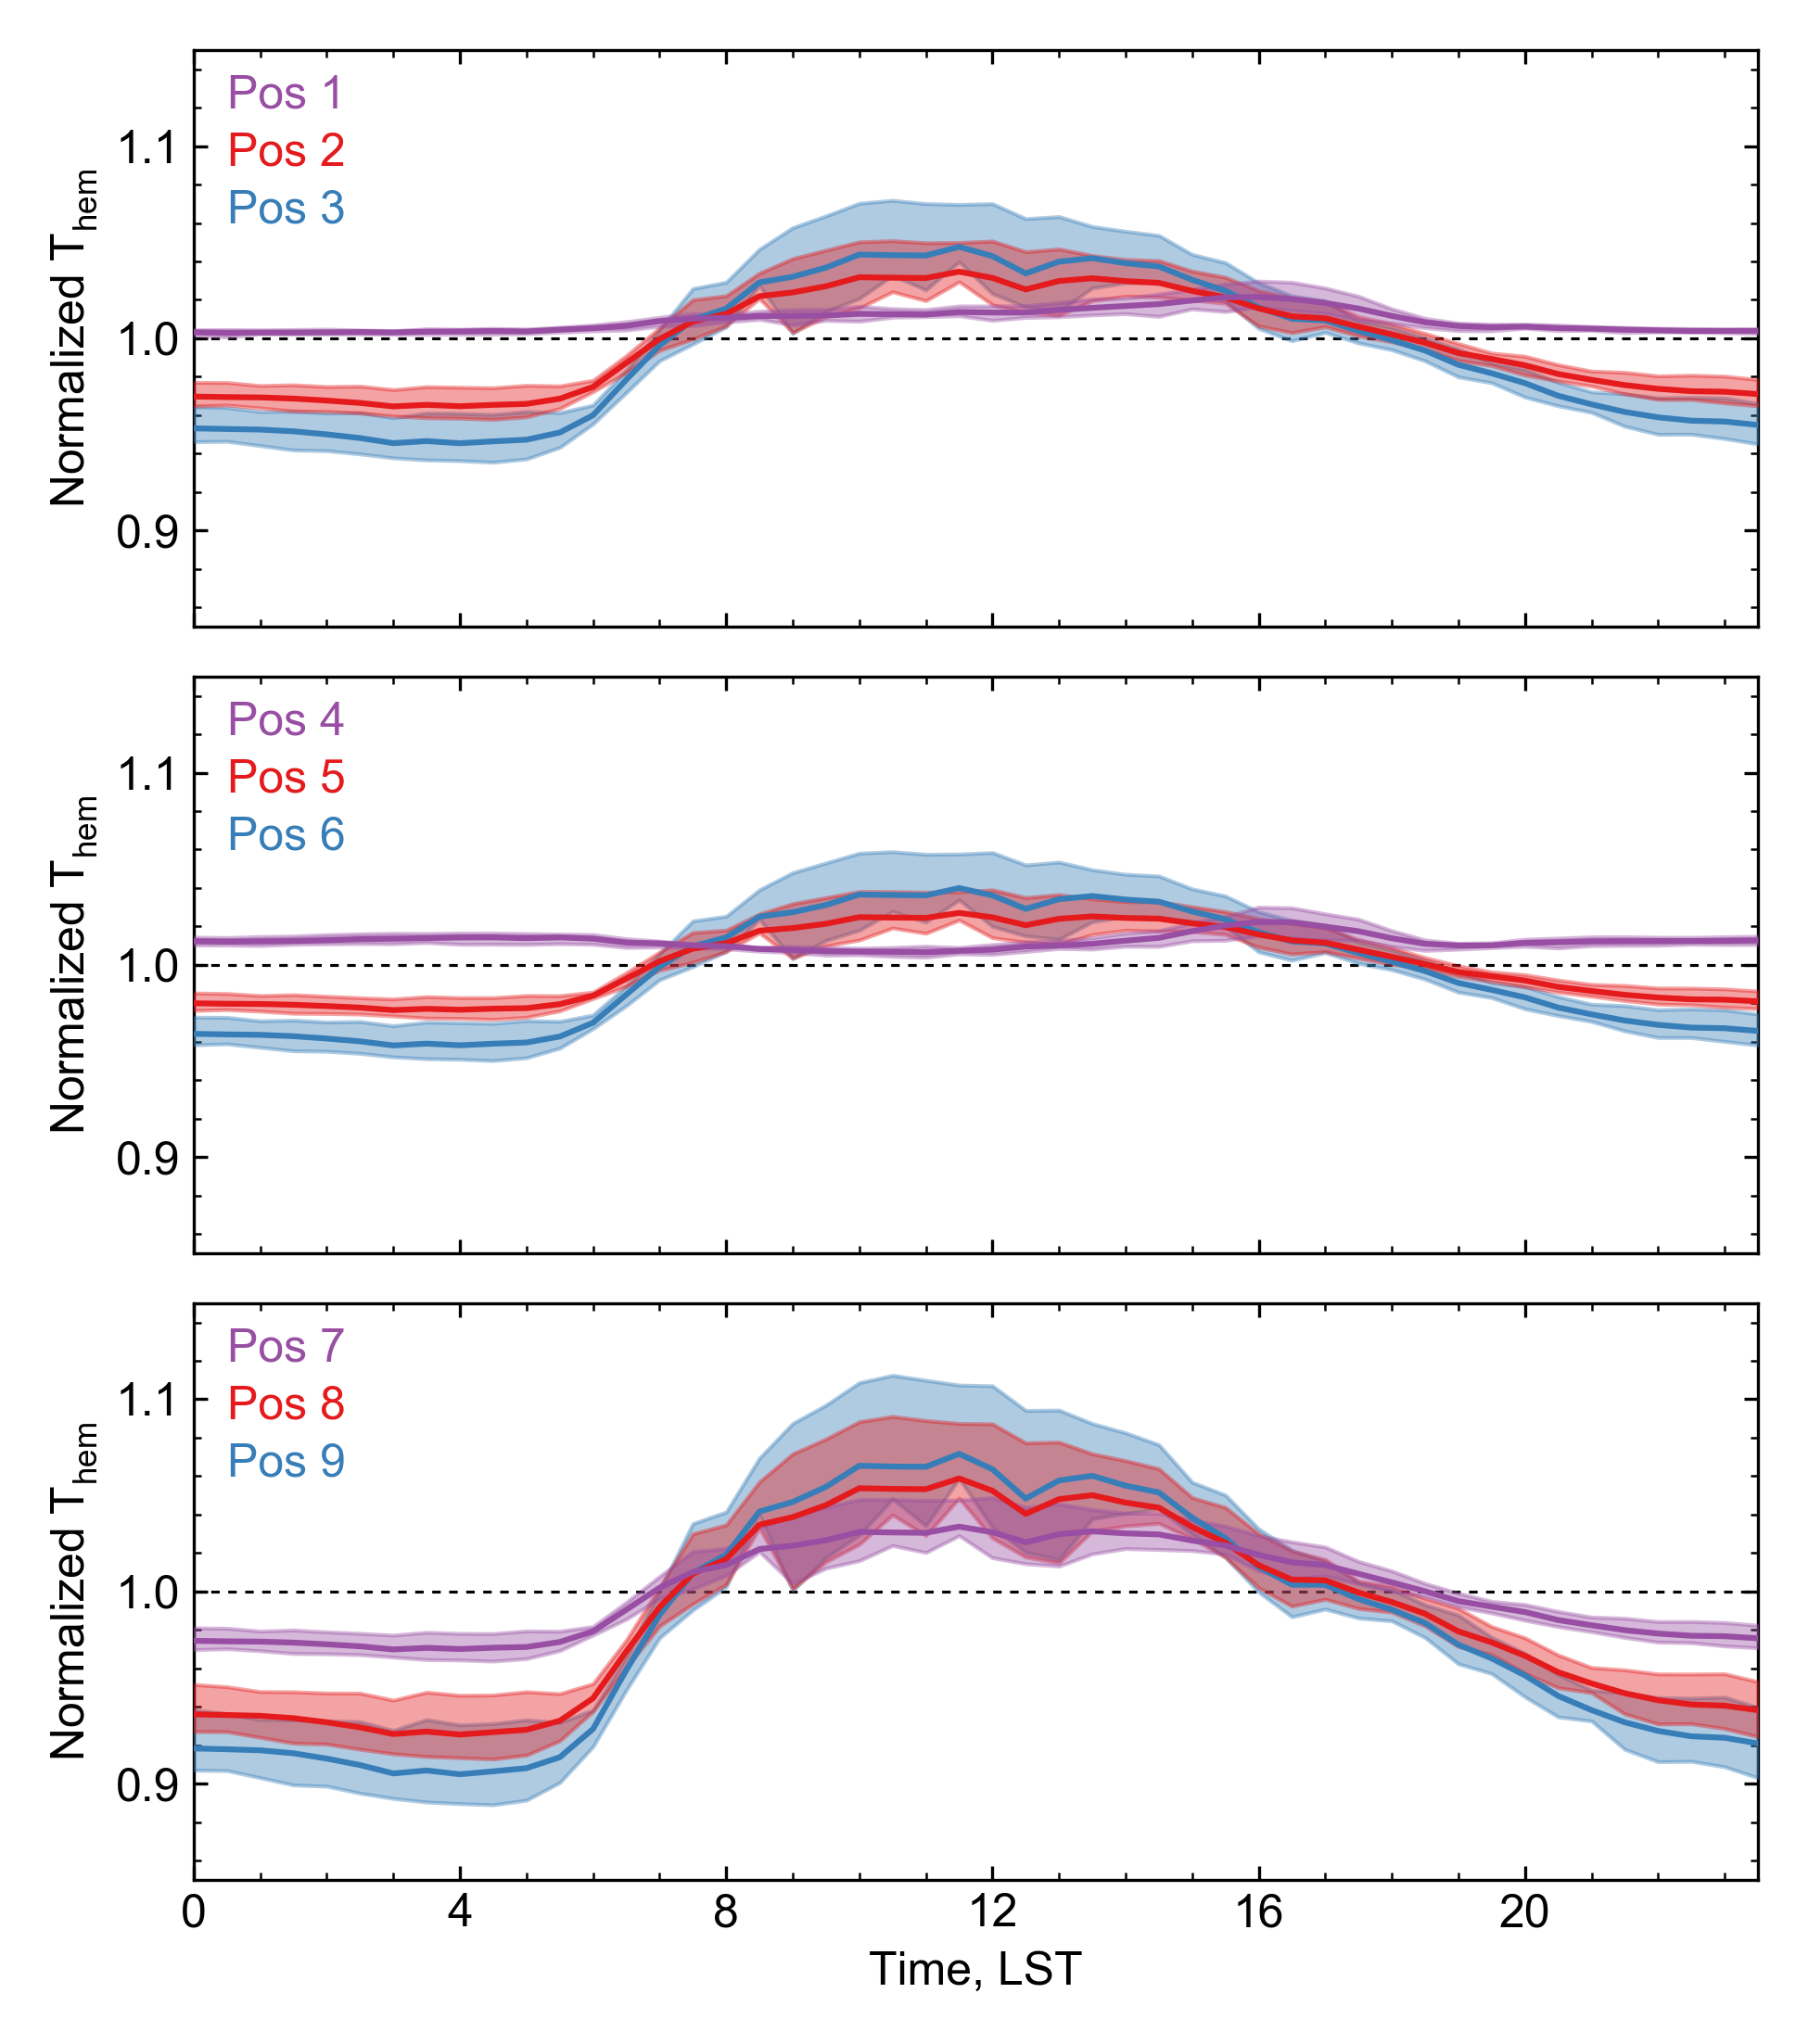
\includegraphics[width=15cm,
 	height=7in,
 	keepaspectratio]{vf_all}
 	\caption{Mean T\textsubscript{hem, r} normalized against T\textsubscript{comp} for each sensor position over the 14-day IOP for a sensor height of 2.17 times mean building height. Shaded area indicates quartiles one through three.}
 	\label{vf_all}
 \end{figure}

  \begin{figure}[H]
	\centering
	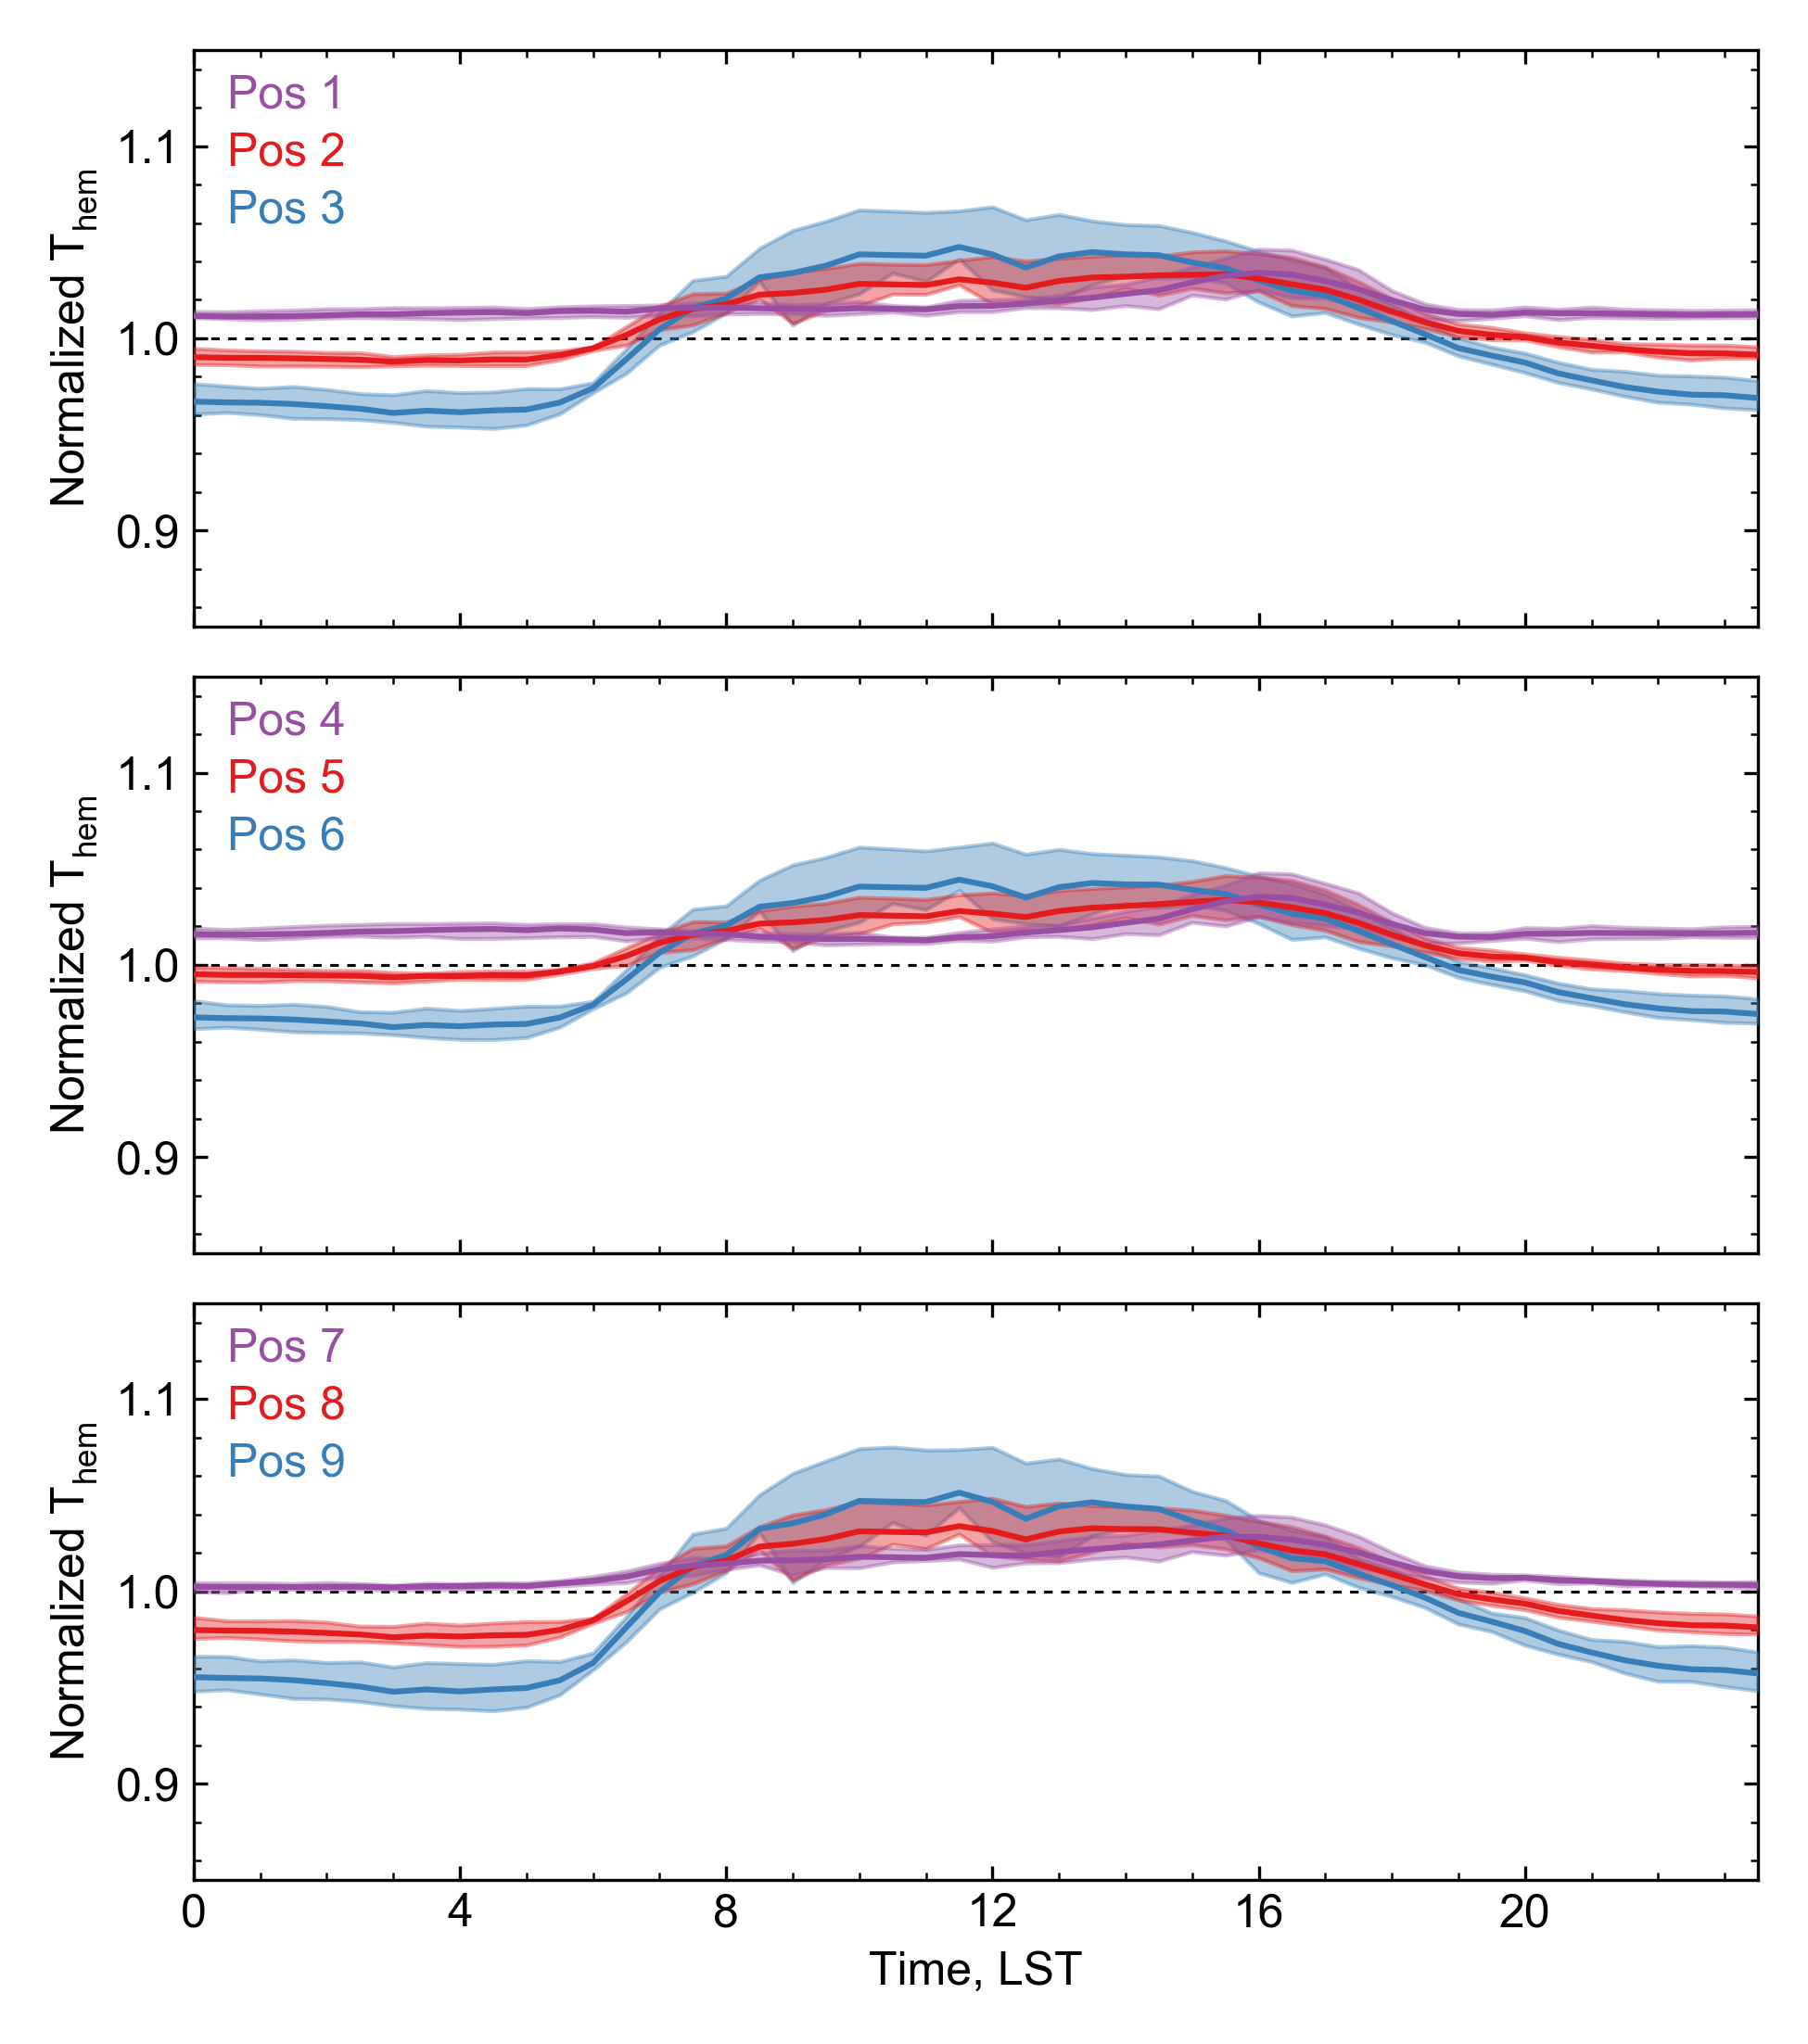
\includegraphics[width=15cm,
	height=7in,
	keepaspectratio]{vf_all45}
	\caption{Mean T\textsubscript{hem, r} normalized against T\textsubscript{comp} for each sensor position over the 14-day IOP for a sensor height of 3 times mean building height. Shaded area indicates quartiles one through three.}
	\label{vf_all45}
\end{figure}
 
Both \citet{Roberts2010} and \citet{Adderley2015} did not find a perfectly representative sensor position for typical low- and mid-rise urban street canyons; this is supported by sensitivity testing performed in this study. As such, under conditions with strong microscale spatial contrasts in T\textsubscript{surf}, T\textsubscript{hem, r} is unlikely to be equal T\textsubscript{comp} regardless of sensor placement. However, sensor view models, such as SUM, can be used to optimize sensor placement with information about surface geometry to retrieve the most accurate measured irradiances and derived T\textsubscript{hem, r} for a given surface geometry.

\section{A practical parameterization}

To save computational time and facilitate broader use of the method, a parameterization scheme was developed to simplify the correction process. In the parameterization, a suite of radiative transfer simulations is run prior to correction (as opposed to at each time step) to retrieve $\tau$ for a range of humidities and path lengths. T\textsubscript{surf} and T\textsubscript{air} are held constant in these simulations as they have a relatively small effect on $\tau$. Simulations for path lengths from 1 to 48 \si{\meter} and water vapor mass densities from 0.1 to 23.5 \si{\gram\per\meter\cubed} are included in Appendix \ref{appendixa}. Sensor-surface geometry is approximated as a single view factor weighted, azimuthally averaged, surface-to-sensor path length calculated using the SUM \citep{Soux2004} and a simplified DBM. This path length represents the average distance from the sensor to the surface as "seen" by the sensor. For each time step, measured humidity is used to infer a hemispherical transmittance ($\overline{\tau_{\Phi}}$) for the approximated surface-sensor geometry. A parameterized T\textsubscript{hem, r} can then be calculated by using measured (in this case, profile averaged) T\textsubscript{air} to decompose measured upwelling longwave into irradiance received by the sensor from the surface $L_{surf}^{at-sensor}$ and from the atmosphere $L_{atm}^{at-sensor}$ via, 

\begin{equation}
	\label{para}
	T_{hem, r~} =\left(\displaystyle\frac{\biggl(\cfrac{\displaystyle L_{surf}^{at-sensor}}{ \displaystyle\tau}\biggr)}{ \displaystyle\sigma}\right)^{0.25}
\end{equation}
\noindent where $\tau$ is calculated using a radiative transfer code and $L_{surf}^{at-sensor}$ is an estimation of the fraction of at sensor measured irradiance emitted by the surface calculated as,

\begin{equation}
	\label{para2}
	\displaystyle L_{surf}^{at-sensor} = L_{total}^{at-sensor} - (1-\tau)\sigma T_{air}^4
\end{equation}

Using this parameterization, a climatology of T\textsubscript{hem, r} for a given surface geometry can be retrieved from approximately 100 simulations as opposed to the many thousands needed for full hemispherical radiative transfer simulation. A variety of online and offline, open and closed source resources are available for radiative transfer simulation \citep{Gastellu-Etchegorry1996,Berk1987,Buehler2005}, some of which are available for free or at a low cost (Spectral-Calc), all of which are likely to provide similar transmittances to those included in Appendix \ref{appendixa}. Figure \ref{para_eval} and Table \ref{parastats} summarize parameterization performance relative to T\textsubscript{hem, r} retrieved via the correction method. Errors are largest during the daytime hours, where the profile averaged T\textsubscript{air} overestimates above canyon T\textsubscript{air} and underestimates near-surface T\textsubscript{air}. Neutral stability in the nighttime and early morning hours reduces these errors significantly as the canyon T\textsubscript{air} profile is approximately isothermal.
 
\begin{figure}[H]
	\centering
	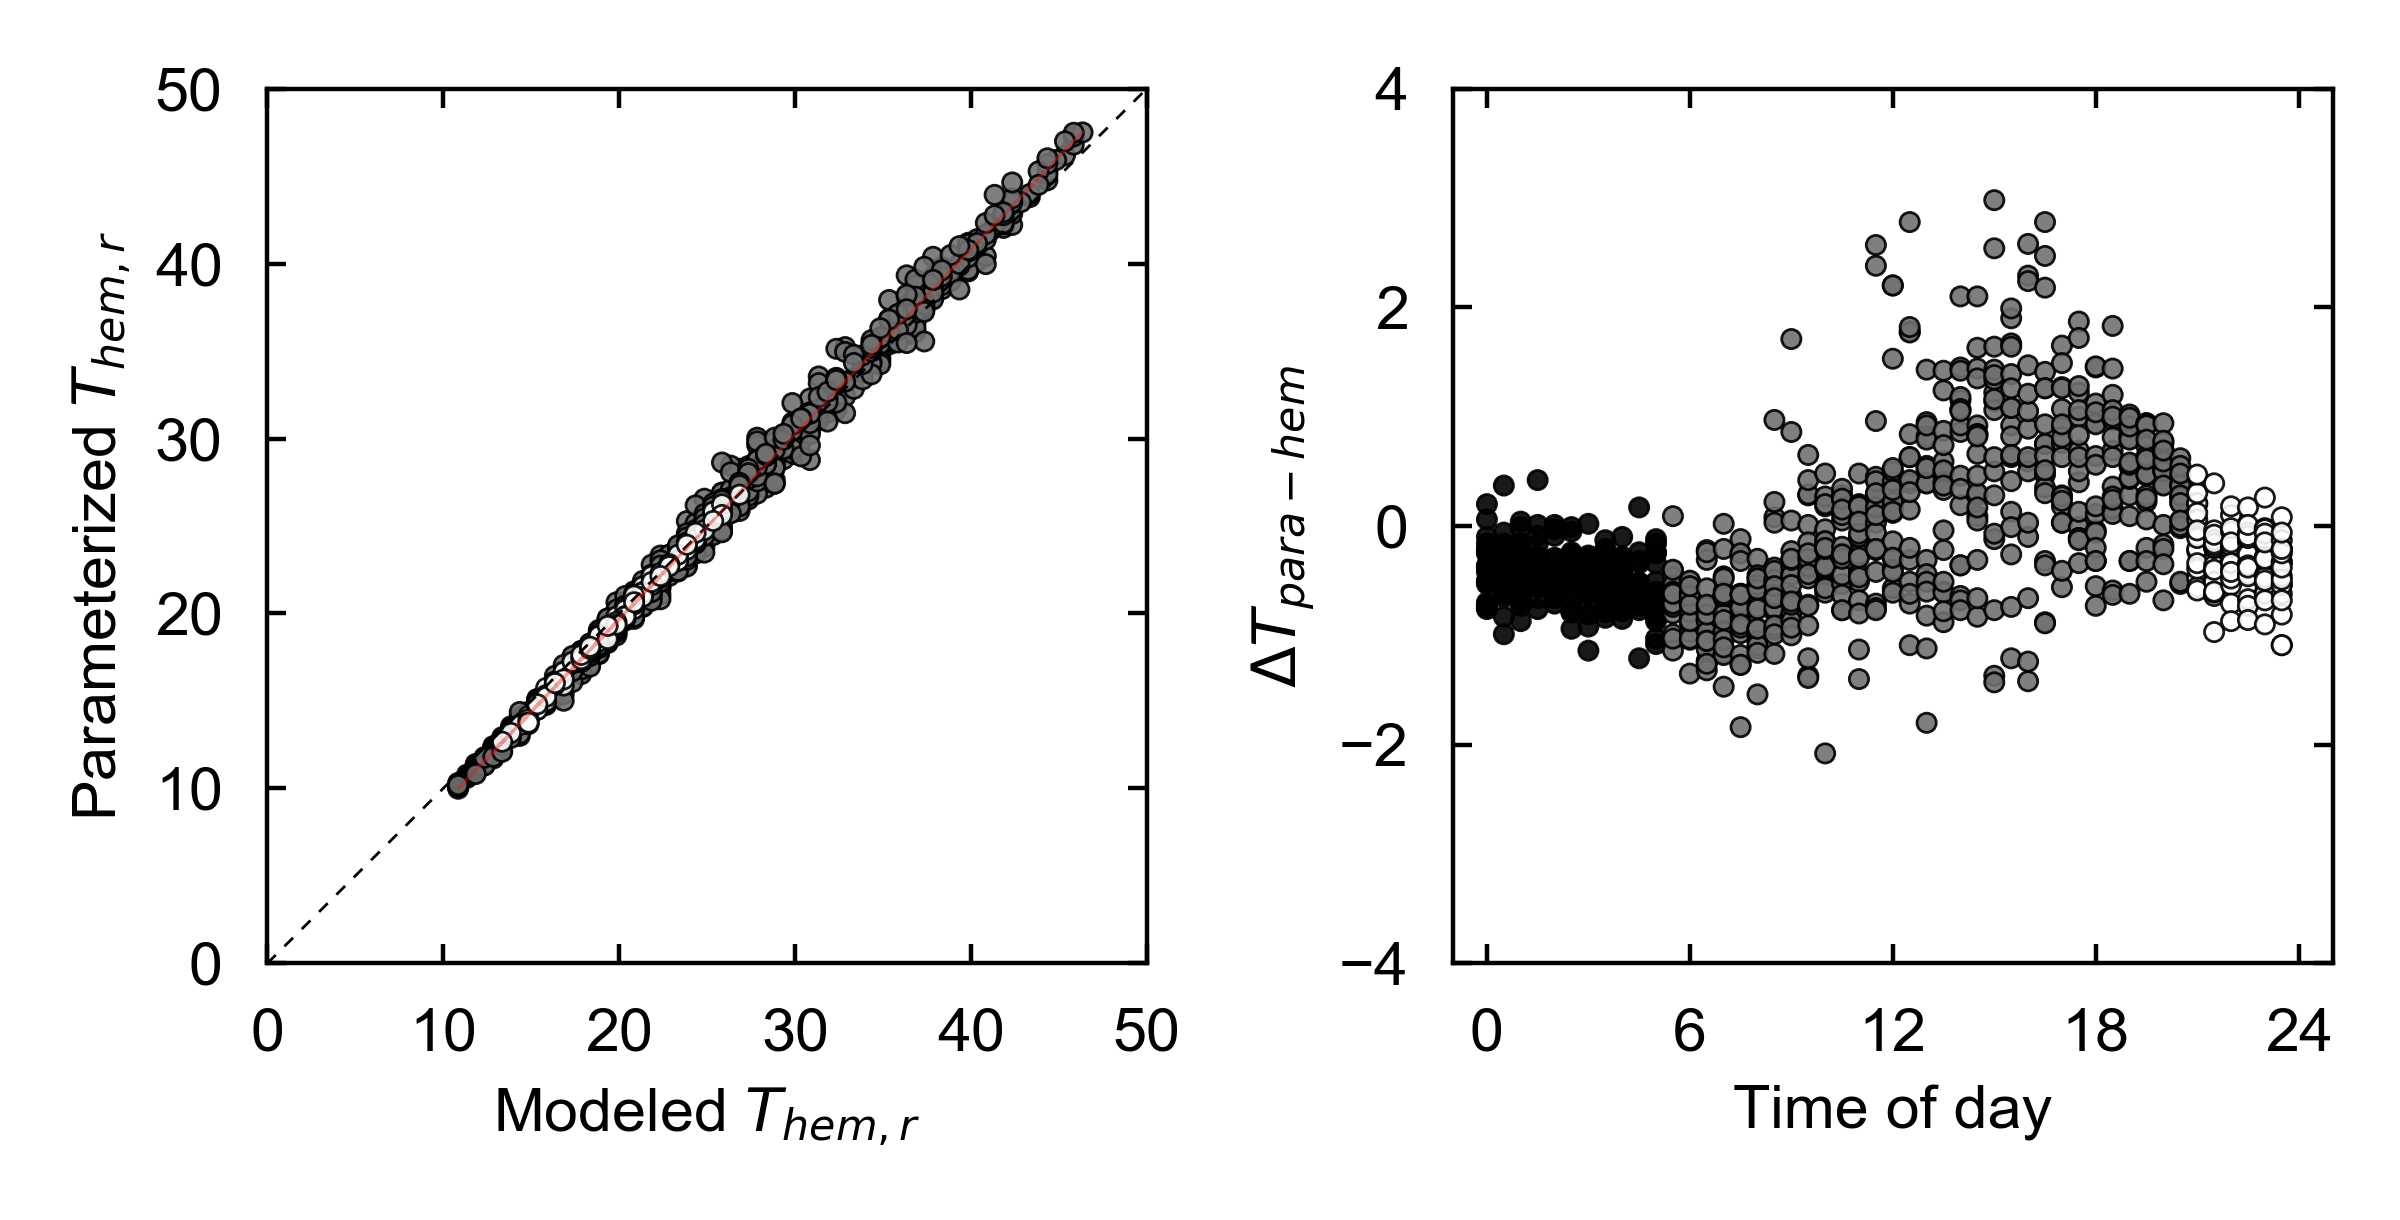
\includegraphics[width=15cm,
	height=7in,
	keepaspectratio]{para_eval}
	\caption{Modeled T\textsubscript{hem, r} versus T\textsubscript{hem, r} derived via the parameterization scheme.}
	\label{para_eval}
\end{figure}
 
\begin{table}[H]
 	\centering
 	\caption{Statistical performance of T\textsubscript{hem} derived using the parameterization scheme relative to modeled T\textsubscript{hem,r}. RMSE\textit{\textsubscript{s}} and RMSE\textit{\textsubscript{u}} represent the systemic and unsystematic RMSE respectively. n = 853}
 	\label{parastats}
 	\begin{tabular}{lcr}
 		\toprule 
 		Statistic & Parameterization & Citation \\  \midrule
 		Slope & 1.058 &  \\ 
 		Intercept, (\si{\kelvin}) & -1.488 &   \\ 
 		\textit{R\textsuperscript{2}} & 0.991 & \\ 
 		MAE,  (\si{\kelvin}) & 0.607& \citep{Willmott1985a} \\ 
 		RMSE,  (\si{\kelvin}) & 0.757 & \citep{Willmott1985a} \\ 
 		RMSE\textit{\textsubscript{s}},  (\si{\kelvin}) & 0.476  & \citep{Willmott1985a} \\ 
 		RMSE\textit{\textsubscript{u}},  (\si{\kelvin}) & 0.588  & \citep{Willmott1985a} \\ 
 		\textit{d}, agreement index & 0.998 & \citep{Willmott2012} \\
 		\bottomrule
 	\end{tabular} 
\end{table}
 
 \section{Conclusions}
 
Accurate, geometrically representative, spatially extensive, and temporally continuous thermal remote sensing of complex terrain (urban or otherwise) is difficult. It is unlikely that a single sensor will satisfy spatial, geometric, and temporal goals. Thus, a combination of satellite, aerial, and in-situ observational methods has been integral in isolating and elucidating the urban effect on surface temperature and its spatial, temporal, and geometric characteristics. However, neither technological advancement nor critical analysis of these methods has provided a satisfactory answer to the questions posed in \citet{Roth1989} viz urban thermal remote sensing. As such, the true spatial, temporal, and geometric nature of the urban effect on surface temperature remains unknown. 
 
This paper details a method for urban T\textsubscript{surf} retrieval using atmospherically corrected hemispherical radiometric surface temperatures derived from continuous near-ground measurements of thermal infrared radiation. Atmospherically corrected, hemispherical urban T\textsubscript{surf} is derived using a method which combines a sensor view model (SUM) to represent urban surface geometry and a point-to-point radiative transfer code (MODTRAN 4.1) to model irradiances upwelling from complex surface terrain in 3-dimensions. At each time step, irradiances are modeled using profiles of T\textsubscript{air} and water vapor content for a range of possible T\textsubscript{hem, r}. Irradiance - T\textsubscript{hem, r} pairings are aggregated into a LUT and the measured irradiance is matched with the closest modeled irradiance to retrieve T\textsubscript{hem, r} for a given time step. Repeated at 30-minute intervals, the method is used to derive an 8-month climatology of urban T\textsubscript{hem, r} from urban irradiances measured as a part of the BUBBLE campaign in Basel, Switzerland.
 
Atmospheric corrections are large and vary significantly based on sensor-surface-sun geometry and synoptic conditions. Thus, T\textsubscript{hem} derived from irradiances measured at different heights or above different surface geometries may have different atmospheric or dome effects that can confound results. This fact makes clear the need for robust atmospheric correction of T\textsubscript{hem} for sUHI analysis or to retrieve radiometric T\textsubscript{hem}. Correction magnitudes are largest on hot, clear sky summertime days --- with large solar input and high T\textsubscript{surf} and T\textsubscript{air} --- and smallest by night and under overcast conditions, during which solar input is suppressed and T\textsubscript{surf} and T\textsubscript{air} are low. Correction magnitudes are most strongly correlated with the T\textsubscript{surf} to T\textsubscript{air} differential and incoming solar radiation and weakly correlated with T\textsubscript{hem, r} and T\textsubscript{air}. Water vapor content did not appear to exert strong control over correction magnitudes.

Comparison of T\textsubscript{surf} from nadir, hemispherical, and complete representations of the Basel Sperrstrasse street canyon show that a hemispherical view is more geometrically representative of the complete surface temperature than a sensor viewing in the nadir. However, sensor placement sensitivity tests show that T\textsubscript{hem, r} varies based on sensor placement and height. Overestimations of T\textsubscript{comp} by T\textsubscript{plan} and T\textsubscript{hem, r} are greatest under clear sky conditions and are much larger for T\textsubscript{plan}. This is particularly important when one considers that satellite observations of urban T\textsubscript{surf} are only possible under clear sky conditions (when T\textsubscript{plan} is least representative of T\textsubscript{comp}). Significant variability in over/underestimation of T\textsubscript{comp} by T\textsubscript{hem, r} and T\textsubscript{plan} based on time of day and synoptic conditions make these biases difficult to generalize to other urban study sites with different surface geometries and characteristics, canyon orientations, and macro climates. However, the measures used to derive T\textsubscript{hem, r} are common to most energy balance assessments and constitute an untapped, but promising, resource to improve understanding of how the built environment affects land T\textsubscript{surf} and to quantify the geometric and temporal biases inherent in satellite TIR remote sensing of complex terrain. 

\cleardoublepage 
\phantomsection  
\renewcommand*{\bibname}{References}
\addcontentsline{toc}{section}{\textbf{References}}

\putbib
\end{bibunit}